% concatenated from main_TIT.tex
\documentclass[onecolumn,ldraftcls, 11pt]{IEEEtran}
%% depending on your installation, you may wish to adjust the top margin:
\addtolength{\topmargin}{9mm}

%%%%%%
%% Packages:
%% Some useful packages (and compatibility issues with the IEEE format)
%% are pointed out at the very end of this template source file (they are 
%% taken verbatim out of bare_conf.tex by Michael Shell).
%
% *** Do not adjust lengths that control margins, column widths, etc. ***
% *** Do not use packages that alter fonts (such as pslatex).         ***
%

\usepackage{pgfplots}
\pgfplotsset{compat=newest}
\usepackage{float}
\usepackage[utf8]{inputenc} 
\usepackage[T1]{fontenc}
\usepackage{url}
\usepackage{ifthen}
\usepackage{cite}
\usepackage{algorithm}
\usepackage{algpseudocode}
\usepackage[cmex10]{amsmath}
\usepackage{wrapfig}
\usepackage{tikz}
\usepackage{circuitikz}
\usepackage{multirow}
\usepackage{makecell}
\usetikzlibrary{shapes, arrows, positioning, patterns}
% Use the [cmex10] option to ensure complicance
                             % with IEEE Xplore (see bare_conf.tex)
\usepackage[includefoot,left=25.4mm,right=26mm,top = 25.4mm, bottom=26mm]{geometry}
% \usepackage[
%     backend=biber,
%     style=ieee,
%   ]{biblatex}

%  \addbibresource{master.bib}
\usepackage[colorlinks=false]{hyperref}%
% \addbibresource{master.bib}
%% Please note that the amsthm package must not be loaded with
%% IEEEtran.cls because IEEEtran provides its own versions of
%% theorems. Also note that IEEEXplore does not accepts submissions
%% with hyperlinks, i.e., hyperref cannot be used.
\usepackage{mleftright}       % fix to wrong spacing of \left-,
\mleftright                   % \middle- \right-commands 
% \renewcommand*{\bibfont}{\footnotesize}
\usepackage{subcaption}
\usepackage{graphicx}         % provides \includegraphics{...} to
                              % include graphics (pdf format)
\usepackage{booktabs}         % fixes poor spacing in tables and
\usepackage{amsthm}
\usepackage{graphics,graphicx,psfrag,color,float}
\usepackage{epsfig,bbold,bbm}
\usepackage{bm}
\usepackage{mathtools}
\usepackage{amssymb}
\usepackage {times}
\usepackage{bbm}
\usepackage{soul}
\usepackage{cleveref}
\usepackage{enumitem}
\usepackage{xcolor}
\usepackage{txfonts}
\makeatletter
\def\namedlabel#1#2{\begingroup
    #2%
    \def\@currentlabel{#2}%
    \phantomsection\label{#1}\endgroup
}
\makeatother
\DeclareUnicodeCharacter{0325}{}
%\newcommand{\Supp}{\operatorname{Supp}}
\newcommand{\comr}[1]{{\textcolor{red}{#1}}}
\newcommand{\comb}[1]{{\textcolor{blue}{#1}}}
\def\QED{\mbox{\rule[0pt]{1.5ex}{1.5ex}}}
\def\endproof{\hspace*{\fill}~\QED\par\endtrivlist\unskip}
\def\argmin{\mathop{\rm argmin}\limits}
\newtheorem{theorem}{\bf{Theorem}}
\newtheorem{fact}{Fact}
\newtheorem{assumption}{Assumption}
\def\wu{\superscript{*}}
\def\wg{\superscript{\dag}}
\newcommand{\supp}{\operatorname{supp}}
\newcommand{\RNum}[1]{\uppercase\expandafter{\romannumeral #1\relax}}
\newcommand{\tab}{\hspace*{2em}}
\newcommand{\beq}{\begin{equation}}
\newcommand{\enq}{\end{equation}}
\newcommand{\bel}{\begin{lemma}}
\newcommand{\enl}{\end{lemma}}

\newcommand{\bet}{\begin{theorem}}
\newcommand{\ent}{\end{theorem}}
\newcommand{\ten}{\textnormal}
\newcommand{\tbf}{\textbf}
\newcommand{\tr}{\mathrm{Tr}}
\newcommand{\vr}{\mathrm{Var}}
\newcommand{\myexp}{{\mathrm{e}}}
\newcommand{\rv}[1]{\mathbf{#1}}
\newcommand{\hilbertspace}[1]{\mathcal{#1}}
\newcommand{\universe}[1]{\mathcal{#1}}
\newcommand{\bound}{\mathsf{bound}}
\newcommand{\nn}{\nonumber}
\newcommand{\E}{\mathbb{E}}
%\newcommand{\tr}{\mathsf{tr\,}}
\newcommand{\ketbra}[1]{|#1\rangle\langle#1|}
\newcommand{\lab}{\mathrm{lab}}
\newcommand{\girth}{\mathrm{girth}}
\newcommand{\pseudoedge}[1]{\stackrel{#1}{\longrightarrow}}
\newcommand{\floor}[1]{\left\lfloor #1 \right\rfloor}
\newcommand{\ceil}[1]{\left\lceil #1 \right\rceil}
\newcommand{\myexponent}{\frac{1}{\floor{n/4}}}
\DeclareMathOperator*{\bigplus}{\text{\Large $+$}}
\newcommand{\customfootnotetext}[2]{{% Group to localize change to footnote
  \renewcommand{\thefootnote}{#1}% Update footnote counter representation
  \footnotetext[0]{#2}}}% Print footnote text
\newcommand{\eps}{\varepsilon}
\newcommand*{\bbone}{\mathbb{1}}
\newcommand*{\bbC}{\mathbb{C}}
\newcommand*{\bbA}{\mathbb{A}}
\newcommand*{\bbR}{\mathbb{R}}
\newcommand*{\bbH}{\mathbb{H}}
\newcommand*{\bbM}{\mathbb{M}}
\newcommand*{\bbF}{\mathbb{F}}
\newcommand*{\bbB}{\mathbb{B}}
\newcommand*{\bbD}{\mathbb{D}}
\newcommand*{\bbG}{\mathbb{G}}
\newcommand*{\bbI}{\mathbb{I}}
\newcommand*{\bbJ}{\mathbb{J}}
\newcommand*{\bbK}{\mathbb{K}}
\newcommand*{\bbL}{\mathbb{L}}
\newcommand*{\bbN}{\mathbb{N}}
\newcommand*{\bbP}{\mathbb{P}}
\newcommand*{\bbQ}{\mathbb{Q}}
\newcommand*{\bbS}{\mathbb{S}}
\newcommand*{\bbhS}{\hat{\mathbb{S}}}
\newcommand*{\bbT}{\mathbb{T}}
\newcommand*{\bbX}{\mathbb{X}}
\newcommand*{\bbW}{\mathbb{W}}
\newcommand*{\bbZ}{\mathbb{Z}}
\newcommand*{\bbE}{\mathbb{E}}
\newcommand*{\bbU}{\mathbb{U}}
\newcommand*{\cP}{\mathcal{P}}
\newcommand*{\cC}{\mathcal{C}_{n}}
\newcommand*{\cA}{\mathcal{A}}
\newcommand*{\cR}{\mathcal{R}}
\newcommand*{\cH}{\mathcal{H}}
\newcommand*{\cM}{\mathcal{M}}
\newcommand*{\cF}{\mathcal{F}}
\newcommand*{\cB}{\mathcal{B}}
\newcommand*{\cD}{\mathcal{D}}
\newcommand*{\cG}{\mathcal{G}}
\newcommand*{\cI}{\mathcal{I}}
\newcommand*{\cJ}{\mathcal{J}}
\newcommand*{\cK}{\mathcal{K}}
\newcommand*{\cL}{\mathcal{L}}
\newcommand*{\cN}{\mathcal{N}}
\newcommand*{\cO}{\mathcal{O}}
\newcommand*{\cS}{\mathcal{S}}
\newcommand*{\chS}{\hat{\mathcal{S}}}
\newcommand*{\cT}{\mathcal{T}}
\newcommand*{\cX}{\mathcal{X}}
\newcommand*{\cW}{\mathcal{W}}
\newcommand*{\cZ}{\mathcal{Z}}
\newcommand*{\cE}{\mathcal{E}}
\newcommand*{\cU}{\mathcal{U}}
\newcommand*{\bP}{\mathbf{P}}
\newcommand*{\bV}{\mathbf{V}}
\newcommand*{\bq}{\mathbf{q}}
\newcommand*{\Ib}{\bar{I}}
\newcommand*{\oI}{\overline{I}}
\newcommand*{\bZ}{\mathbf{Z}}
\newcommand*{\G}{\mbox{Good}}
\newcommand*{\Gd}{\mbox{Good_1}}
\newcommand*{\cV}{\mathcal{V}}
\newcommand*{\cY}{\mathcal{Y}}
\newcommand*{\hy}{\hat{y}}
\newcommand*{\hx}{\hat{x}}
\newcommand*{\bX}{\mathbf{X}}
\newcommand*{\bU}{\mathbf{U}}
\newcommand*{\bY}{\mathbf{Y}}
\newcommand*{\bQ}{\mathbf{Q}}
\newcommand*{\cl}{\mathcal{l}}
\newcommand*{\Xb}{\bar{X}}
\newcommand*{\Yb}{\bar{Y}}
%\newcommand*{\bI}{\bar{I}}
\newcommand*{\mximax}[1]{\Xi^\delta_{\max}(P_{#1})}
\newcommand*{\mximin}[1]{\Xi^\delta_{\min}(P_{#1})}
\newcommand{\bra}[1]{\langle #1|}
\newcommand{\ket}[1]{|#1 \rangle}
\newcommand{\braket}[2]{\langle #1|#2\rangle}
\newcommand*{\bx}{\mathbf{x}}
\newcommand*{\by}{\mathbf{y}}
\mathchardef\mhyphen="2D
\newcommand*{\uI}{\underline{I}}
\newcommand*{\uH}{\underline{H}}
\newcommand*{\oH}{\overline{H}}
\newcommand*{\renyi}{R\'enyi }
\newcommand{\ketbrasys}[2]{\overset{#2}{|#1\rangle\langle#1|}}
\newcommand{\argmax}{\operatornamewithlimits{arg\ max}}
\newcommand{\norm}[2]{{\left\lVert #1 \right\rVert}_{#2}}
\newcommand{\abs}[1]{\left\vert#1\right\vert}
%\newcommand*{\uI}{\underline{I}}
\newcommand\plainnorm[1]{\lVert#1\rVert}
\pagestyle{plain}
\newcommand*{\enc}{\mathrm{enc}}
\newcommand*{\dec}{\mathrm{dec}}
\newcommand*{\denc}{\mathrm{d-enc}}
 \newcommand\Fontvi{\fontsize{6}{7.2}\selectfont}
  \newcommand\Montvi{\fontsize{10}{7.2}\selectfont}
  \newcommand\qontvi{\fontsize{8.5}{7.2}\selectfont}
\makeatletter
\newcommand*{\rom}[1]{\expandafter\@slowromancap\romannumeral #1@}
\makeatother
% \DeclareMathOperator*{\bigplus}{\text{\huge ++}}
\mathchardef\mhyphen="2D
\newlist{steps}{enumerate}{1}
\setlist[steps, 1]{leftmargin = 1.1cm, label = Step \arabic*.}
\newtheorem{remark}{Remark}
\newtheorem{definition}{Definition}
\newtheorem{claim}{Claim}
\newtheorem{conjecture}{Conjecture}
%\newtheorem{fact}{Fact}
% \newcommand\norm[1]{\left\lVert#1\right\rVert}

\newtheorem{comment}{Remark}
% \newtheorem{theorem}{Theorem}
\newtheorem{lemma}{Lemma}
\newtheorem{corollary}{Corollary}
\newtheorem{proposition}{Proposition}

% \newtheorem{theorem}{Theorem}[section]
% \newtheorem{corollary}{Corollary}[theorem]
% \newtheorem{lemma}[theorem]{Lemma}



% Use the [cmex10] option to ensure complicance
                             % with IEEE Xplore (see bare_conf.tex)

%% Please note that the amsthm package must not be loaded with
%% IEEEtran.cls because IEEEtran provides its own versions of
%% theorems. Also note that IEEEXplore does not accepts submissions
%% with hyperlinks, i.e., hyperref cannot be used.

\interdisplaylinepenalty=2500 % As explained in bare_conf.tex


%%%%%%
% correct bad hyphenation here
\hyphenation{op-tical net-works semi-conduc-tor}
\newcommand{\mh}[1]{{\textcolor{blue}{#1}}}

% ------------------------------------------------------------
\begin{document}
%\title{upper-bounds on Generalization Error of Quantum Learning Algorithms via Quantum R\'enyi Divergences}

\title{Quantum Information Ordering and Differential Privacy}

\author{
  Naqueeb Ahmad Warsi\textsuperscript{$*$}, Ayanava Dasgupta\textsuperscript{$*$} and  Masahito Hayashi\textsuperscript{$\dagger$}
 % \textsuperscript{$\dagger$}
%}

}


\customfootnotetext{$*$}{
Indian Statistical Institute,
Kolkata 700108, India.
Email: 
{\sf 
 naqueebwarsi@isical.ac.in, ayanavadasgupta\_r@isical.ac.in
}
}

\customfootnotetext{$\dagger$}{School of Data Science, The Chinese University of Hong Kong, Shenzhen, Longgang District, Shenzhen, 518172, China

International Quantum Academy, Futian District, Shenzhen 518048, China

Graduate School of Mathematics, Nagoya University, Nagoya, 464-8602, Japan.
Email: 
{\sf hmasahito@cuhk.edu.cn}}


\maketitle
\begin{abstract}
    We study quantum differential privacy (QDP) by defining a notion of the order of informativeness between pairs of quantum states. In particular, we show that if the hypothesis testing divergence of one pair dominates over that of the other pair, then this dominance holds for every $ f$-divergence. This approach completely characterizes $(\eps,\delta)$-QDP mechanisms by identifying the most informative $(\eps,\delta)$-DP quantum state pairs. We apply this to study precise limits for privatized hypothesis testing and privatized quantum parameter estimation, including tight upper-bounds on the quantum Fisher information under QDP. Finally, we establish near-optimal contraction bounds for differentially private quantum channels with respect to the hockey-stick divergence.
\end{abstract}


\begin{IEEEkeywords}
hypothesis testing, quantum differential privacy, Blackwell's ordering, SLD Fisher's information, hockey stick R\'enyi divergence.
\end{IEEEkeywords}

\section{Introduction}\label{sec_intro}

The trade-off between extracting useful insights by an investigator and preserving a respondent's privacy lies at the heart of modern quantum machine learning. While classical Differential Privacy (DP) \cite{dwork2006calibrating,dwork2006} provides a rigorous framework to limit adversarial inference via hypothesis testing, extending these guarantees to the quantum regime presents unique challenges. Recent advances in Quantum Differential Privacy (QDP) \cite{ZY2017} have made non-trivial attempts \cite{DHLTL21,HRF23,AK25,Nuradha24,Nuradha25} to understand differentially private mechanisms in the quantum setting. In this manuscript, we advance the understanding of quantum differential privacy by grounding QDP in the geometry of asymmetric hypothesis testing. We establish a universal information ordering for differentially private mechanisms, proving that the entire privacy regime can be analyzed by a single ``most-informative'' pair of quantum states. Leveraging this, we derive exact, mechanism-agnostic limits for different statistical tasks: the optimal error exponent in hypothesis testing, the maximum achievable Fisher information for parameter estimation, and the fundamental contraction of distinguishability under private quantum channels.


{\em Framework for Differential Privacy.---}
In the quantum setting, differential privacy constrains the \emph{output} which the quantum algorithms produce. Formally, consider a scenario where a respondent prepares a quantum system in state $\tau \in \{\rho, \sigma\}$. The pair $(\rho, \sigma)$ satisfies $(\eps, \delta)$-DP if, for any general quantum measurement (POVM) performed by an investigator, the probability distributions of the measurement outcomes are statistically close. Thus, as defined in \cite{ZY2017} for fixed $\eps \geq 0$ and $\delta \in [0,1]$, $(\rho, \sigma)$ is $(\eps, \delta)$-DP if they satisfy the following.
\begin{definition}\label{def_DP_state}
   For every POVM measurement $0 \preceq \Lambda \preceq \mathbb{I}$, the following holds:
    \begin{equation}
        \begin{split}
            \tr[\Lambda \rho] &\leq e^{\eps} \tr[\Lambda \sigma]+ \delta,\\
        \tr[\Lambda \sigma] &\leq e^{\eps} \tr[\Lambda \rho]+ \delta.
        \end{split}\label{def_DP_state_eq}
    \end{equation}
    Further, we denote $\mathfrak{D}_{(\eps,\delta)}$ to be the collection of all pairs of quantum states that satisfy \eqref{def_DP_state_eq}. Moreover, for $\delta = 0$, we denote $(\rho,\sigma)$ to be pure $\eps$-DP or just $\eps$-DP i.e. $(\rho,\sigma) \in \mathfrak{D}_{(\eps,0)}$.
\end{definition}

For the case when $\delta = 0$, any value of $\eps$ satisfying Eq. \eqref{def_DP_state_eq} must be at least $\max\{D_{\max}(\rho\|\sigma),\, D_{\max}(\sigma\|\rho)\},$ where $D_{\max}$ denotes the max-relative entropy. As a consequence, the required $\eps$ is typically very large, which severely weakens privacy as discussed in the section below. To mitigate this issue, one introduces a positive additive constant $\delta$, allowing the permissible value of $\eps$ to be significantly reduced. Further in Eq. \eqref{def_DP_state_eq}, if we consider only binary POVMs then it motivates us to analyze QDP from the point of view of binary quantum hypothesis testing.

\noindent {\em The Operational Scenario: The Respondent and the Investigator.---}
This manuscript is based on the strategic interaction between two distinct parties: the \textbf{Respondent} (the data owner) and the \textbf{Investigator} (the adversary).

The \textbf{Respondent} serves as the gatekeeper of a sensitive database containing potential datasets $S$ and $T$, which differ solely by the presence of a single individual $A$, such that $S \setminus (S \cap T) = \{A\}$. To make data accessible while maintaining confidentiality, the Respondent instantiates a statistical \textbf{oracle} (the mechanism). This oracle operates as a conditional distribution $\mathbb{P}^{(D)}(O\mid I)$---or in the quantum setting, a quantum channel---generating an output $O$ for a specific query $I$ based on the underlying dataset $D \in \{S,T\}$. The Respondent's primary objective is to configure this oracle to satisfy strict differential privacy constraints, effectively masking the specific identity of the dataset.

The \textbf{Investigator} operates as the \textbf{Adversary} in this setting. They interact with the Respondent's oracle by issuing queries and processing the resulting outputs. Their goal is to execute a binary hypothesis test to breach privacy: specifically, to distinguish whether the underlying dataset is $S$ or $T$, thereby revealing the presence of individual $A$. The central thesis of this work is that the ``informativeness'' of the Respondent's oracle dictates the success of the Investigator: the more useful the oracle is for legitimate statistical utility, the more vulnerable it is to this adversarial attack. We structure our contributions in three steps corresponding to this dynamic: the privacy limit (comparing the Respondent's oracles), the adversarial extraction limit (the Investigator's power), and the channel analysis (the properties of the Respondent's defense mechanism).

{\em First step: Privacy.}
The primary objective of differential privacy is to ensure that the outputs of the oracle corresponding to two neighboring inputs are difficult for the Investigator to distinguish. This implies a direct inverse relationship: the more informative the oracle is about the datasets, the less private it is. To formalize this, we require a rigorous method to compare the ``informativeness'' of different oracles. We consider a pair of oracles modeled as $\bbP^{(D)}(O\mid I)$ and $\bbQ^{(D)}(O\mid I)$. We say that $\bbP^{(D)}(O\mid I)$ is more informative than $\bbQ^{(D)}(O\mid I)$ (represented as the order $\bbP^{(D)}(O\mid I) \succeq \bbQ^{(D)}(O\mid I)$ or simply $\bbP^{(D)}(O\mid I)$ dominates $\bbQ^{(D)}(O\mid I)$) if the pair $\{\bbP^{(S)}(O\mid I),\bbP^{(T)}(O\mid I)\}$ is statistically easier to  distinguish as compared to the pair $\{\bbQ^{(S)}(O\mid I),\bbQ^{(T)}(O\mid I)\}$.


In $1951$, Blackwell \cite{Blackwell51,BG54} formalized this notion of comparing ``informativeness'' for classical statistical experiments. He showed that $\bbP^{(D)}(O\mid I) \succeq \bbQ^{(D)}(O\mid I)$ if and only if there exists a Markov kernel (stochastic map) $\cM$ such that $\bbQ^{(S)}(O\mid I) = \cM(\bbP^{(S)}(O\mid I))$ and $\bbQ^{(T)}(O\mid I) = \cM(\bbP^{(T)}(O\mid I))$. Further, using the data-processing inequality (monotonicity property) we have $D_{f}(\bbP^{(S)}(O\mid I)\| \bbP^{(T)}(O\mid I)) \geq D_{f}(\bbQ^{(S)}(O\mid I)\| \bbQ^{(T)}(O\mid I))$, where $D_f$ is the $f$-divergence \cite{Sason_2016}. For the case when these oracles are differentially private (with the same privacy parameters), it is obvious that the above monotonicity would help us obtain security bounds of the less informative in terms of the one that is more informative.

Likewise, in the quantum domain, we consider two quantum oracles whose outputs are $\{\rho^{S},\rho^{T}\}$ and $\{\sigma^{S},\sigma^{T}\}$. We say that $\{\rho^{S},\rho^{T}\}$ is more informative than $\{\sigma^{S},\sigma^{T}\}$ if the former is statistically easier for the Investigator to distinguish. However, a significant theoretical hurdle arises here: unlike the classical case, it follows from \cite{GLW24} and \cite{Matsumoto2014} that the statistical ordering $\{\rho^{S},\rho^{T}\} \succeq \{\sigma^{S},\sigma^{T}\}$ does \emph{not} imply the existence of a completely positive trace-preserving (CP-TP) map---or even a positive trace-preserving map---that transforms the former into the latter. As a consequence, we cannot rely on the standard data-processing inequalities of quantum $f$-divergences \cite{Hirche_2024} to transfer bounds. We overcome this in Theorem \ref{theo_QLDP_approx_F_div_bound} by proving that an explicit channel (a CP-TP map) construction is unnecessary. We show that if the quantum hockey stick divergence \cite{Sharma09} between the oracle outputs $\{\rho^{S},\rho^{T}\}$ dominates $\{\sigma^{S},\sigma^{T}\}$ for every parameter, then the inequality $D_{f}(\rho^{S}\|\rho^{T}) \geq D_{f}(\sigma^{S}\|\sigma^{T})$ holds universally. This result allows us to define a ``worst-case'' (most informative) pair of states that characterizes the upper bound on the Investigator's adversarial capability.

{\em Second step: Information extraction under privacy constraints.}
We now analyze, under the $(\eps,\delta)$-DP constraints, the fundamental limits of the \textbf{Investigator's} ability to extract information from \textbf{Respondent's} data. Here, we treat the Investigator as an adversary whose goal is to infer the hidden parameter or state. We investigate this statistical inference using our quantum $f$-divergence dominance result (Theorem \ref{theo_QLDP_approx_F_div_bound}). The Investigator's success in guessing the hidden parameter is strictly limited by the privacy constraints imposed by the mechanism. We examine this limit through two adversarial viewpoints: binary hypothesis testing and parameter estimation.

In the former scenario, we begin with the one-shot setting, where the Investigator attempts to distinguish between two nearby sources $\rho_{\theta_0}$ and $\rho_{\theta_1}$ (parametrized by two private parameters $\theta_1$ and $\theta_2$) after their encoding has been privatized through an $(\eps,\delta)$-DP mechanism. This scenario exposes the operational limit of privacy breaches. We show that, among all $(\eps,\delta)$-DP mechanisms, the Investigator's optimal performance—quantified by the \emph{hypothesis testing divergence}—is maximized by the ``weakest'' (most informative) privatized mechanism permitted by the definition. This optimality carries over to KL, hockey stick R\'enyi (see Definition \ref{def_quant_renyi_hockey}), and measured R\'enyi divergences. We then extend the analysis to the asymptotic regime and establish that this same privatized mechanism determines the optimal error exponent. This yields a unified characterization: the privacy requirement compresses the geometry of the state space, imposing a fundamental ceiling on the Investigator's probability of successfully distinguishing hypotheses.

In the regime of parameter estimation, the limit of the Investigator’s ability to pinpoint the private parameter is measured by the Fisher information. In the quantum case, we use the Symmetric Logarithmic Derivative (SLD) Fisher information \cite{Hiai1991}. By leveraging the idea of our ``weakest'' (most informative) private method, we determine the exact maximum SLD Fisher information the Investigator can obtain while the mechanism respects the $(\eps, \delta)$-DP rule. This result improves on past studies that only looked at the simpler case where $\delta=0$ \cite{YH20}, and sets a hard physical limit on how accurately an adversarial Investigator can estimate sensitive parameters under the privacy condition.

{\em Third step: The Quantum Channel.}
Finally, we analyze the mechanism itself by studying quantum channels which are $(\eps,\delta)$-DP. From the adversarial perspective, the channel acts as a defense mechanism that suppresses the distinguishability of inputs. We quantify this suppression via the \emph{contraction of divergence}---comparing the divergence of the output distributions induced by $(\eps,\delta)$-DP channels to the divergence of the input states; see, for example, \cite{Asoodeh24}, \cite{ZA23}, and the references therein.
This contraction is studied using an integral representation involving the hockey stick divergence \cite{Sason_2016}. We leverage our framework to first establish an almost tight upper bound on the contraction coefficient of any $(\eps,\delta)$-DP CP-TP map with respect to the hockey stick divergence.

A crucial technical contribution in this step addresses the difficulty of the $\delta > 0$ regime. The additive $\delta$ term typically complicates the analysis of entropic quantities. We observe that, similar to the classical case, there exists a \emph{pure} $(\eps + \log(1/1-\delta))$-DP pair of distributions that can be obtained by \emph{truncating} the original $(\eps,\delta)$-DP pair. We formally extend this to the quantum domain, showing that this truncated pair is close ($O(\delta)$ in $L_1$ distance) to the original pair. We use this truncated pair to obtain a meaningful upper bound on the relative entropy of the original $(\eps,\delta)$-DP pair using the continuity of relative entropy. This upper bound recovers the known result for $\delta=0$ \cite{KOV15,DRS22} as a special case.
Moreover, these contraction-based analyses serve to connect the channel-level action with both privacy guarantees and the limits on adversarial extraction. By bounding how much input distinctions are suppressed at the output, we obtain direct, worst-case control of output distinguishability (useful for bounding the success of hypothesis-testing attacks) and of output information quantities (limiting the precision of Fisher-information-based estimation).


\begin{table}[h]
\caption{Relationship between results obtained in this work and related studies}\label{tab}
\begin{center}
\begin{tabular}{|c|c|c|c|c|}
\hline
 \multirow{2}{*}{Results} & \multicolumn{2}{|c|}{Classical Domain} & \multicolumn{2}{|c|}{Quantum Domain}\\
\cline{2-5} 
&{$\eps$-DP} & {$(\eps,\delta)$-DP} & {$\eps$-DP} & {$(\eps,\delta)$-DP}\\
 \hline
\makecell{Existence of Weakest \\ DP Mechanism} & \makecell{\cite[Theorem 5]{KOV15}} & \makecell{\cite[Theorem 18]{KOV15}} & \makecell{\cite[Theorem 2]{YH20}}  & \makecell{Lemma \ref{lemma_diff_priv_quant} \\ of this manuscript.}\\
\hline
\makecell{ Data Processing based\\ upper-bounds using Weakest\\ DP Mechanism} & {\makecell{\cite[Lemma D.8]{DRS22}}}  & & \makecell{ Corollary \ref{theo_QLDP_F_div_pure_bound} \\ of this manuscript.} & \makecell{Theorem \ref{theo_QLDP_approx_F_div_bound} \\ of this manuscript.} \\
\hline
\makecell{Privatized Hypothesis \\ Testing} 
&
\makecell{\cite[Theorem 18]{KOV15}}
 & 
\cite[Theorem 18]{KOV15}
& \makecell{\cite[Section \RNum{2}B]{YH20}} & \makecell{Theorem \ref{THJ} \\ and Corollary \ref{Cor12}\\ of this manuscript.}\\
\hline
\makecell{Privatized Parameter \\ Estimation} 
&
\makecell{\cite[Theorem 18]{KOV15}}
 & 
\cite[Theorem 18]{KOV15}
& \makecell{\cite[Section  \RNum{2}A]{YH20}} & \makecell{Theorem \ref{theo_fisher_info_bound} \\ of this manuscript.}\\
\hline
\makecell{Privatized Contraction\\  Coefficient of Trace Distance} & \cite[Corollary 11]{KOV15} & & \makecell{\cite[Theorem $2$]{Nuradha25}} & \makecell{\cite[Theorem $5$]{Nuradha25}}\\
\hline
\makecell{Contraction Coefficient\\ of Hockey-stick Divergence} & \makecell{\cite[Theorem 1]{ZA23}} & \makecell{Corollary \ref{corr_contrac_classical_hockey_stick} \\ of this manuscript.} & \makecell{\cite[Theorem 1]{Nuradha25}}  & \makecell{Lemma \ref{lemma_contrac_hockey_stick} \\ of this manuscript.} \\
\hline
\makecell{Contraction Coefficient based \\ Upper-bounds on Relative entropy\\ of LDP channels } & & \makecell{Theorem \ref{theorem_classical_kl_bound} \\ of this manuscript.} & \cite[Proposition 3]{Nuradha25} & \\
\hline  
\end{tabular}
\end{center}
\end{table}

\subsection{Organization of this Manuscript and our Contributions}
The rest of this manuscript is organized as follows:
\begin{itemize}
    \item In Section~\ref{sec_def_not}, we list the essential notations, definitions, and facts which will be used throughout this manuscript. 

   \item In Section~\ref{sec_char_region}, we provide a geometric characterization of the privacy region of $(\eps,\delta)$-QDP and provide a construction of the weakest (most informative) $(\eps,\delta)$-DP pair of quantum states.
    \item In Section~\ref{sec_diff_priv_quant}, we first define a notion of order of informativeness between two pairs of quantum states via quantum hypothesis testing divergence. Using this ordering, in Theorem \ref{lemma_t_hyp_F_Div}, we give an $f$-divergence dominance of a more informative pair of quantum states over a lesser informative pair of quantum states. Further, in Lemma~\ref{lemma_DP_t_hyp_rel}, we show that a pair of quantum states is $(\eps,\delta)$-differentially private if and only if  $D^{\alpha}_{H} {(\rho\|\sigma)} \leq -\log \max\left\{1 - \delta - e^{\eps}\alpha, e^{-\eps}(1 -\delta - \alpha),0\right\}$ for any $\alpha \in [0,1],$ where $D^{\alpha}_{H} {(\rho\|\sigma)}$ is the hypothesis testing divergence between $\rho$ and $\sigma.$ Using this in Lemma~\ref{lemma_diff_priv_quant},  we identify an explicit ``weakest'' (most-informative) pair of $(\eps,\delta)$-DP quantum states that dominates all others. Finally, in Theorem \ref{theo_QLDP_approx_F_div_bound}, we show that the $f$-divergence of any pair of $(\eps,\delta)$-DP quantum states can be upper-bounded by that of the ``weakest'' (most-informative) pair of $(\eps,\delta)$-DP quantum states.
 
    \item In Section~\ref{sec:fisher}, we apply our framework to the regime of the quantum hypothesis testing and the quantum parameter estimation under privacy constraints. In particular, in Theorem \ref{THJ}, we show that among all $(\eps,\delta)$-DP mechanisms, the hypothesis testing divergence is maximized by the weakest (most informative) privatized mechanism. Further, in Theorem~\ref{theo_fisher_info_bound}, we derive the exact maximum SLD Fisher information achievable by any $(\eps,\delta)$-DP mechanism.

    \item In Section~\ref{sec_LDP_channel}, we analyze the contraction of divergences under differentially private channels. In Lemma~\ref{lemma_contrac_hockey_stick}, we obtain nearly tight upper and lower bounds on the contraction coefficient of $(\eps,\delta)$-LDP channels with respect to the quantum hockey-stick divergence. We then use this to derive a novel upper-bound on the relative entropy for classical $(\eps,\delta)$-LDP channels in Theorem~\ref{theorem_classical_kl_bound} via its integral representation \cite{Sason_2016}.
\end{itemize}

Table \ref{tab} above summarizes the relation between the results obtained in our manuscript and the existing results. 




\section{Notations, Definitions and Facts}\label{sec_def_not}

We use $\cH$ to denote a finite-dimensional Hilbert space and we denote its dimension with $\abs{\cH}$, $\mathcal{D}(\cH)$ to represent the set of all density matrices acting on $\cH$. For any quantum state $\rho \in \cD(\cH)$, we define $\mbox{supp}(\rho):=\mbox{Span}\{\ket{i}\mid \lambda_{i}> 0\},$ where $\left\{\lambda_i\right\}$ represent non-zero eigenvalues of $\rho$. For any finite and non-empty set $\cX$, we denote $\cP(\cX)$ as the set of all probability distributions over $\cX$. Similarly, for any distribution $P \in \cP(\cX)$, we denote $\mbox{supp}(P):=\{x\in \mathcal{X}\mid P(x)>0\}.$ 

\begin{definition}[Classical minimum type-\RNum{2} error]\label{def_min_type2_err}
    Given a pair of probability distributions $P_1,P_2$ over a finite set $\cX$, the minimum type-\RNum{2} error of a fixed order $\alpha \in [0,1]$ is defined as follows,
    \begin{equation}
        \beta(\alpha|P_1\|P_2) := \min_{\substack{\phi: \cX \to [0,1]\\ \sum_{x \in \cX} P_1(x)\phi(x) \leq \alpha}} 1 - \sum_{x \in \cX} P_2(x)\phi(x).\label{def_min_type2_err_eq}
    \end{equation}
\end{definition}


\begin{definition}[Classical hypothesis testing divergence]\label{def_hyp_div}
    For any pair of probability distributions $P,Q$ over a finite set $\cX$, and for any $\alpha \in [0,1]$, the classical hypothesis testing divergence of order $\alpha$ is defined as
    \begin{equation}
        D^{\alpha}_{H}(P\|Q) := \max_{\substack{\phi: \cX \to [0,1]\\ \sum_{x \in \cX} P(x)\phi(x) \leq \alpha}} -\ln \left( 1 - \sum_{x \in \cX} Q(x)\phi(x) \right).
    \end{equation}

    Further, note that for any $\alpha \in [0,1]$, $D^{\alpha}_{H}(P\|Q) = -\ln \beta(\alpha,P,Q)$ where $\beta(\alpha,P,Q)$ is as defined in Definition \ref{def_min_type2_err}.
\end{definition}


\begin{definition}[Classical hockey-stick divergence{\cite{Hull2003}}]\label{def_class_hockey_stick}
Let $P$ and $Q$ be probability distributions on a finite (or measurable) space $\mathcal{X}$, and let $\gamma \geq 1$.  
Then, the hockey-stick divergence between $P$ and $Q$ is defined as
\[
  E_{\gamma}(P \| Q)
  := \sup_{A \subseteq \mathcal{X}} \Big( P(A) - \gamma \, Q(A) \Big)
  = \sum_{x \in \mathcal{X}} \big[ P(x) - \gamma Q(x) \big]_+ ,
\]
where $[t]_+ := \max\{t,0\}$ denotes the positive part of $t$.
\end{definition}

\begin{definition}[Classical alpha divergence]\label{def_c-alpha_div}
    For any pair of probability distributions $P,Q$ over a finite set $\cX$, and for any $\alpha \in [0,1]$, the classical $\alpha$ divergence of order $\alpha$ is defined as
    \begin{equation}
        D_{\alpha}(P\|Q) := 
        \frac{1}{\alpha-1} \log \sum_{x \in \cX} P(x)^\alpha Q(x)^{1-\alpha}.
    \end{equation}
\end{definition}

\begin{definition}\label{def_data_proc_div_class}
    A function $\bbD : \cP(\cX) \times \cP(\cX) \to \bbR^{+}$ (where $\cX$ is an arbitrary set of finite cardinality) is called a divergence if for  
    any classical channel $\cK: \cX \to \cY$, (where $\cY$ is another arbitrary set of finite cardinality), the following holds,
    \begin{equation}
       \bbD(P_1\|P_2) \geq  \bbD(\cK(P_1)\|
       \cK(P_2)), \forall P_1,P_2 \in \cP(\cX),\label{def_data_proc_div_class_eq}
    \end{equation}
    where for each $i = 1,2$, $\cK(P_i)(y) := \bbE_{X \sim P_i} \left[\cK(y\mid X)\right]$.
\end{definition}



\begin{definition}[Quantum minimum type-\RNum{2} error]\label{Q-def_min_type2_err}
    For any $\rho,\sigma \in \cD(\cH_A)$, 
    the minimum type-\RNum{2} error of a fixed order $\alpha \in [0,1]$ is defined as follows,
    \begin{equation}
        \beta(\alpha|\rho\|\sigma) := 
        \min_{\substack{0 \preceq \Lambda \preceq \bbI:\\
        \tr[\Lambda \rho] \leq \alpha}} 
        \tr[(\bbI - \Lambda)\sigma] .\label{Qdef_min_type2_err_eq}
    \end{equation}
\end{definition}

\begin{definition}[Quantum hypothesis testing divergence {\cite{Wang_2012}}]\label{d_hyp_func}
    For any $\rho,\sigma \in \cD(\cH_A)$, for any $\alpha \in [0,1]$, the quantum hypothesis testing divergence $D^{\alpha}_{H}{(\rho\|\sigma)}$ of order $\alpha$ is defined as follows,
    \begin{equation}
        D^{\alpha}_{H}{(\rho\|\sigma)} := \max_{\substack{0 \preceq \Lambda \preceq \bbI:\\
        \tr[\Lambda \rho] \leq \alpha}} -\ln \tr[(\bbI - \Lambda)\sigma] .\label{d_hyp_func_eq}
    \end{equation}
\end{definition}

\begin{definition}[Quantum hockey stick divergence \cite{SW12}]\label{f_sym_hyp_func}
    For any $\rho,\sigma \in \cD(\cH_A)$, we define the quantum hockey stick divergence $E_{\gamma}(\rho\|\sigma)$ of order $\gamma\geq 0$ as follows,
    \begin{equation}
        E_{\gamma}(\rho\|\sigma) := \max_{\substack{0 \preceq \Lambda \preceq \bbI}
        }\tr[\Lambda (\rho - \gamma\sigma)].\label{f_sym_hyp_func_eq}
    \end{equation}
\end{definition}

\begin{definition}[\cite{Hirche_2024}]\label{def_f_div_integral_rep}
    Consider $\cF$ be the set of functions $f : (0,\infty) : \to \bbR$ that are convex and twice differentiable with $f(1) = 0$. Then, for any $f \in \cF$ and for any $\rho,\sigma \in \cD(\cH_A)$, we define the quantum $f$-divergence $D_f(\rho\|\sigma)$ as follows,
    \begin{equation}
        D_f(\rho\|\sigma) :=  \int_{1}^{\infty}\left( f''(\gamma) E_{\gamma}(\rho\|\sigma) + \gamma^{-3} f''(\gamma^{-1}) E_{\gamma}(\sigma\|\rho)\right) d\gamma.\label{def_f_div_integral_rep_eq}
    \end{equation}
    whenever, the integral is finite and $D_{f}(\rho\|\sigma) := +\infty$ otherwise.
\end{definition}

\begin{definition}\label{def_quant_KL_div}
    Consider $\rho,\sigma \in \cD(\cH_A)$, then, we define the quantum Divergence between $\rho$ and $\sigma$ as follows
    \begin{equation*}
        D(\rho \| \sigma) := \begin{cases}
            \tr[\rho(\log\rho -\log\sigma)], &\text{  if } \rho \ll \sigma, \\
             +\infty, &\text{ else}.
        \end{cases}
    \end{equation*}
\end{definition}

\begin{definition}[Hockey Stick R\'enyi Divergence {\cite{Hirche_2024}}]\label{def_quant_renyi_hockey}
    Consider $\rho,\sigma \in \cD(\cH_A)$ and $\alpha \in [0,1) \cup (1,+\infty)$. Then, hockey stick R\'enyi Divergence of order $\alpha$ between $\rho$ and $\sigma$ is defined as follows,
        \begin{align}
    D_\alpha(\rho \| \sigma) &:= \frac{1}{\alpha - 1} \log \big( 1 + (\alpha - 1) H_\alpha(\rho \| \sigma) \big),
\label{def_P_div_integral_rep_eq} \\
H_\alpha(\rho \| \sigma) &:= \alpha \int_{1}^{\infty} \gamma^{\alpha - 2} E_\gamma(\rho \| \sigma) + \gamma^{-\alpha - 1} E_\gamma(\sigma \| \rho) \, \mathrm{d}\gamma,
    \end{align}
when a parameter $\alpha \in [0,1) \cup (1,+\infty)$
satisfies the condition
$\alpha < 1 \cap \rho \not\perp \sigma$ or the condition $\rho \ll \sigma$.
\end{definition}

\begin{definition}[Measured R\'enyi Divergence {\cite{H2017QIT,Hirche_2024}}]\label{def_sand}
    Consider $\rho,\sigma \in \cD(\cH_A)$ and $\alpha \in [0,1) \cup (1,+\infty)$. Then, measured R\'enyi Divergence of order $\alpha$ between $\rho$ and $\sigma$ is defined as follows,
    \begin{align*}
        \check{D}_{\alpha} (\rho \| \sigma) 
:= \sup_{M: {\rm POVM}}D_\alpha(P^M_\rho\|P^M_\sigma),
    \end{align*}
    where $P^M_\rho$ is the distribution given as
    $P^M_\rho(i):= \tr \rho M_i$ for a POVM $M=\{M_i\}_i$.    
\end{definition}


\begin{definition}\label{def_data_proc_func}
    A function $\varmathbb{D} : \cD(\cH_A) \times \cD(\cH_A) \to \bbR^{+}$ (where $\cH_A$ is any arbitrary Hilbert space of finite dimension) is called a divergence if for  
    any completely positive trace preserving (CP-TP) map $\cE: \cH_A \to \cH_B$, (where $\cH_B$ is another arbitrary Hilbert space of finite dimension) the following holds,
    \begin{equation}
       \varmathbb{D}(\rho_1\|\rho_2) \geq  \varmathbb{D}(\cE(\rho_1)\|\cE(\rho_2)), \forall \rho_1,\rho_2 \in \cD(\cH_A).\label{def_data_proc_quantum_div_eq}
    \end{equation}
\end{definition}

\begin{fact}
\label{fact_hockey_approx}
 For any two  pair  $(P,Q)$ and $(P',Q')$ probability distributions, the following holds for any $\gamma \geq 1$,
 \begin{align}
     E_{\gamma}(P'\|Q') &\leq E_{\gamma}(P\|Q) + \frac{1}{2}\norm{P'-P}{1} + \frac{\gamma}{2}\norm{Q'-Q}{1}.\label{fact_hockey_approx_eq1}
 \end{align}
\end{fact}
\begin{proof}
    From Definition \ref{def_class_hockey_stick}, we have
    \begin{align*}
        E_{\gamma}(P'\|Q') &\overset{(a)}{=}  P'(A) - \gamma Q'(A)\\
        &\leq  P(A) - \gamma Q(A) +  P'(A) - P(A) +\gamma(Q'(A) - Q(A))\\
        &\leq \max_{B \subseteq\cX}(P(B) - \gamma Q(B)) + \max_{C \subseteq\cX} (P'(C) - P(C)) +\gamma\max_{D \subseteq\cX}( Q'(D) - Q(D))\nn\\
        &=E_{\gamma}(P\|Q) +  \frac{1}{2}\norm{P'-P}{1} +\frac{\gamma}{2}\norm{Q'-Q}{1}.
    \end{align*}
    where in $(a)$, let $A$ be the maximal set for  $E_{\gamma}(P'\|Q')$ according to Definition \ref{def_class_hockey_stick}. This proves Fact \ref{fact_hockey_approx}.
\end{proof}


\begin{fact}[H\"older's inequality]\label{holder_classic}
    For any two vectors $x=(x_1, \dots, x_n)$ and $y=(y_1, \dots, y_n)$ in $\mathbb{R}^n$ and for any real numbers $p,q \in [1,\infty)$ such that $\frac{1}{p}+\frac{1}{q} = 1$, we have,
    \begin{equation}
        \sum_{i=1}^n \abs{x_i y_i} \leq \left(\sum_{i=1}^n \abs{x_i}^p\right)^{1/p}\left(\sum_{i=1}^n \abs{y_i}^q\right)^{1/q}.\label{Holder_fact_classical}
    \end{equation}
    Further, for the case when $p =1$ and $q = \infty$, the right-hand side of \eqref{Holder_fact_classical} can be interpreted as follows,
    \begin{equation}
        \left(\sum_{i=1}^n \abs{x_i}^p\right)^{1/p}\left(\sum_{i=1}^n \abs{y_i}^q\right)^{1/q} = \left(\sum_{i=1}^n \abs{x_i}\right) \max_{i \in [n]} \abs{y_i}.\label{Holder_fact_classical_p1_qinf}
    \end{equation}
\end{fact}


\begin{fact}[\cite{Sason_2016}]\label{fact_classical_KL_div_integral_rep}
Let $P$ and $Q$ be probability distributions on a finite (or measurable) space $\mathcal{X}$. Then, the classical relative entropy (Kullback-Leibler divergence) admits the following integral representation in terms of the classical hockey-stick divergence:
\begin{equation}
    D(P\|Q) = \int_{1}^{\infty} \left( \frac{1}{\gamma} E_{\gamma}(P\|Q) + \frac{1}{\gamma^2} E_{\gamma}(Q\|P) \right) d\gamma,
\end{equation}
where $E_{\gamma}(P\|Q)$ is the classical hockey-stick divergence as defined in Definition~\ref{def_class_hockey_stick}.
\end{fact}

\begin{fact}\label{fact_d_hyp_func}
    For any $\rho,\sigma \in \cD(\cH_A)$, for any $\alpha \in [0,1]$, the quantum hypothesis testing divergence $D^{\alpha}_{H}{(\rho\|\sigma)}$ of order $\alpha$ satisfies the following,
    \begin{equation}
        D^{\alpha}_{H}{(\rho\|\sigma)} = - \log \beta(\alpha|\rho\|\sigma),\label{fact_d_hyp_func_eq}
    \end{equation}
    where for any $\alpha \in [0,1]$, $\beta(\alpha|\rho\|\sigma)$ is defined in Definition \ref{Q-def_min_type2_err}.
\end{fact}

\begin{fact}[\cite{Hirche_2024}]\label{fact_f_div_integral_rep}
    For any $f \in \cF$ (where $\cF$ is defined in Definition \ref{def_f_div_integral_rep}) and for any $\rho,\sigma \in \cD(\cH_A)$, we have,
    \begin{equation}
        D_f(\rho\|\sigma) :=  \int_{0}^{\infty} f''(\gamma) E_{\gamma}(\rho\|\sigma) d\gamma,\label{fact_f_div_integral_rep_eq}
    \end{equation}
    where $D_f(\rho\|\sigma)$ is defined in Definition \ref{def_f_div_integral_rep}.
\end{fact}

\begin{fact}[\cite{Hirche_2024}]\label{fact_KL_div_integral_rep}
    For any $\rho,\sigma \in \cD(\cH_A)$, and setting $f =x\log x$ in Definition \ref{def_f_div_integral_rep}, we have the following integral representation of the quantum relative entropy $D(\rho\|\sigma)$,
    \begin{equation}
        D(\rho\|\sigma) =  \int_{0}^{\infty}\left( \frac{1}{\gamma} E_{\gamma}(\rho\|\sigma) + \frac{1}{\gamma^2} E_{\gamma}(\sigma\|\rho)\right) d\gamma.\label{fact_KL_div_integral_rep_eq}
    \end{equation}
\end{fact}

\begin{fact}[\cite{Hirche_2024}]\label{fact_P_div_integral_rep}
    For any $\rho,\sigma \in \cD(\cH_A)$, 
    we have the following relation between
        hockey-stick R\'enyi Divergence $D_\alpha(\rho\|\sigma)$ and measured R\'enyi Divergence $\check{D}_\alpha(\rho\|\sigma)$,
    \begin{align}
    \check{D}_\alpha(\rho \| \sigma) \le D_\alpha(\rho \| \sigma) ,
    \label{fact_P_div_integral_rep_eq} 
    \end{align}
for a parameter $\alpha \in [0,1) \cup (1,+\infty)$.
\end{fact}

\begin{fact}
\label{fact:commuting_renyi_full}
Let $\rho$ and $\sigma$ be two commuting quantum states on a Hilbert space $\mathcal{H}$ (i.e., $[\rho, \sigma] = 0$). For any order $\alpha \in (0, \infty) \setminus \{1\}$, the Hockey Stick R\'enyi divergence coincides with the Measured R\'enyi divergence:
\begin{equation}
    D_{\alpha}(\rho \| \sigma) = \check{D}_{\alpha}(\rho \| \sigma) = \frac{1}{\alpha-1} \log \left( \sum_i p_i^\alpha q_i^{1-\alpha} \right),
\end{equation}
where $\{p_i\}$ and $\{q_i\}$ are the eigenvalues of $\rho$ and $\sigma$ in their common eigen-basis.
\end{fact}




\begin{fact}\label{T_hyp_func_equi}
    For any $\rho,\sigma \in \cD(\cH_A)$, for any $\alpha \in [0,1]$, we have the following equality,
    \begin{equation}\beta(\alpha|\rho\|\sigma) =
        \min_{\substack{0 \preceq \Lambda \preceq \bbI:\\
        \tr[\Lambda \rho] \leq \alpha}} \tr[(\bbI - \Lambda)\sigma] = \min_{\substack{0 \preceq \Lambda \preceq \bbI:\\
        \tr[\Lambda \rho] = \alpha}} \tr[(\bbI - \Lambda)\sigma].
        \label{T_hyp_func_equi_eq}
    \end{equation}
\end{fact}

\begin{proof}
    Given any $\alpha \in [0,1]$, we consider a POVM $\{\Tilde{\Lambda},\bbI - \Tilde{\Lambda}\}$, (where $0 \preceq \Tilde{\Lambda} \preceq \bbI$) such that $\tr[\Tilde{\Lambda} \rho] = \alpha' < \alpha$ for some $\alpha' \in (0,1)$. We denote $\beta' := \tr[(\bbI - \Tilde{\Lambda})\sigma]$ and $\delta := \frac{1 -\alpha}{1-\alpha'} \in (0,1)$. We now consider an operator $\hat{\Lambda} := \bbI -\delta\left(\bbI -\Tilde{\Lambda}\right)$. The facts $\delta \in (0,1)$ and $\left(\bbI - \Tilde{\Lambda}\right) \preceq \bbI$ yield that $0\preceq \hat{\Lambda} \preceq \bbI$. Thus, $\{\hat{\Lambda},\bbI - \hat{\Lambda}\}$ forms a valid POVM, for which $\tr[\hat{\Lambda} \rho] = 1 - \delta(1-\alpha') = \alpha$ and
    \begin{align*}
        \tr[(\bbI - \hat{\Lambda})\sigma] = \delta \tr[(\bbI - \Tilde{\Lambda})\sigma]
      \overset{(a)}{<} \beta',
    \end{align*}
    where $(a)$ follows from the fact that $\delta < 1$ and $\beta' = \tr[(\bbI - \Tilde{\Lambda})\sigma]$. Thus, for any POVM $\{\Tilde{\Lambda},\bbI - \Tilde{\Lambda}\}$,  such that $\tr[\Tilde{\Lambda} \rho] < \alpha$, there exists a POVM $\{\hat{\Lambda},\bbI - \hat{\Lambda}\}$ such that $\tr[\Tilde{\Lambda} \rho] = \alpha$ and $\tr[(\bbI - \hat{\Lambda})\sigma] < \tr[(\bbI - \Tilde{\Lambda})\sigma]$. Therefore, the optimum $\Lambda$ in the LHS of \eqref{T_hyp_func_equi_eq} satisfies $\tr[{\Lambda} \rho] = \alpha$. This proves Fact \ref{T_hyp_func_equi}.
\end{proof}


\begin{fact}[\cite{SW12}]\label{Fact_hockey_equiv_form}
    For any $\rho,\sigma \in \cD(\cH_A)$, the quantum hockey stick divergence $E_{\gamma}(\rho\|\sigma)$ of order $\gamma \geq 0$ (see Definition \ref{f_sym_hyp_func}) has the following equivalent form,
    \begin{equation}
        E_{\gamma}(\rho\|\sigma) = \tr|(\rho - \gamma\sigma)|_{+},\label{Fact_hockey_equiv_form_eq}
    \end{equation}
    where $|\cdot|_{+}$ denotes the positive part of the operator, i.e., $|O|_{+} := \sum_{i} \max\{0,\lambda_i\}\ketbra{\psi_i}$, where $\lambda_i$ and $\ket{\psi_i}$ are the eigenvalues and eigenvectors of $O$, respectively.
\end{fact}



\begin{fact}[{\cite[Lemma $3.1$]{BST2019}}]\label{fact_state_trans}
Let $\rho_1, \sigma_1 \in \mathcal{S}(\mathbb{C}^2)$ be commuting qubit quantum states and 
let $\rho_2, \sigma_2 \in \mathcal{S}(\mathbb{C}^d)$.  
Then the following two conditions are equivalent:
\begin{enumerate}
    \item There exists a CP-TP map $\mathcal{E} : \mathcal{S}(\mathbb{C}^2) \to \mathcal{S}(\mathbb{C}^d)$ such that 
    $\mathcal{E}(\rho_1) = \rho_2$ and $\mathcal{E}(\sigma_1) = \sigma_2$;
    \item $D_{\max}(\rho_1 \Vert \sigma_1) \ge D_{\max}(\rho_2 \Vert \sigma_2)$ 
    and $D_{\max}(\sigma_1 \Vert \rho_1) \ge D_{\max}(\sigma_2 \Vert \rho_2)$.
\end{enumerate}
\end{fact}


\begin{fact}\label{T_hyp_func_equi2}
    For any $\rho,\sigma \in \cD(\cH_A)$, for any $\alpha \in [0,1]$ the following equality holds,
    \begin{equation}
        \max_{\substack{0 \preceq \Lambda \preceq \bbI:\\
        \tr[\Lambda \rho] \geq \alpha}} \tr[(\bbI - \Lambda)\sigma] = \max_{\substack{0 \preceq \Lambda \preceq \bbI:\\
        \tr[\Lambda \rho] = \alpha}} \tr[(\bbI - \Lambda)\sigma].\label{T_hyp_func_equi2_eq}
    \end{equation}
\end{fact}

\begin{proof}
    Proof of Fact \ref{T_hyp_func_equi2} follows directly from the proof of Fact \ref{T_hyp_func_equi}.
\end{proof}






\begin{fact}\label{fact_DP_hockey_rel}
    Consider $\rho,\sigma \in \cD(\cH_A)$. Then, for any $\eps \geq 0,\delta \in [0,1)$, the following statements are equivalent, 

    \textbf{(1)} $\rho$ and $\sigma$ satisfies,
    \begin{equation}
        \tr[\Lambda \rho] \leq e^{\eps} \tr[\Lambda \sigma]+ \delta, \mbox{~for any } 0 \preceq \Lambda \preceq \bbI. \label{fact_DP_hockey_rel_eq}
    \end{equation}

    \textbf{(2)} $ E_{e^\eps}(\rho\|\sigma) \leq \delta$, where $E_{e^\eps}(\cdot\|\cdot)$ is the quantum hockey stick divergence (see Definition \ref{f_sym_hyp_func}) of order $e^\eps$.
\end{fact}





\section{Characteristic Region of $(\eps,\delta)$-Differentially Private Quantum Mechanisms}\label{sec_char_region}
In this section, we introduce the concept of the characteristic region of a quantum mechanism that satisfies $(\eps,\delta)$-quantum differential privacy (QDP) as defined in \cite[Definition $2$]{ZY2017}. The characteristic region provides a geometric representation of the trade-offs between the privacy parameters $\eps$ and $\delta$ for a given private quantum mechanism. To illustrate this concept, consider a hypothesis test between two quantum states $\rho$ and $\sigma$ over a finite dimensional Hilbert space $H$ as follows,
\begin{align}
    H &:= \begin{cases}
        H_0: \mbox{Given quantum state is} ~\rho,  \\
        H_1: \mbox{Given quantum state is} ~\sigma. 
    \end{cases}
\end{align}

Under the choice of a rejection POVM $0\preceq \Lambda \preceq \bbI$ for $H_0$, the type-I error is given by $\alpha_{\Lambda} := \tr\left[\Lambda \rho\right]$ and the type-II error is given by $\beta_{\Lambda} := 1 - \tr\left[\Lambda \sigma\right]$.
Now, for any pair  $(\rho,\sigma)$ of quantum states, the characteristic region is defined as follows,

\begin{definition}\label{def_char_region}
    For any pair of quantum states $(\rho,\sigma)$, the characteristic region $\cR(\rho,\sigma)$ is defined as follows,
    \begin{equation}
        \cR(\rho,\sigma) := \left\{(\alpha_{\Lambda},\beta_{\Lambda}) : 0 \preceq \Lambda \preceq \bbI\right\}.\label{def_char_region_eq}
    \end{equation}
\end{definition}

Further, if $(\rho,\sigma)$ is $(\eps,\delta)$-QDP, then for any rejection POVM $\Lambda$, from \eqref{def_DP_state_eq} the following constraints hold,
\begin{align}
    \beta_{\Lambda} &\geq e^{-\eps}(1-\delta -\alpha_{\Lambda}),\label{char_region_eq1}\\
    \beta_{\Lambda} &\geq 1 -\delta - e^{\eps}\alpha_{\Lambda},\label{char_region_eq2}\\
    \beta_{\Lambda} &\leq 1 - e^{-\eps}(\alpha_{\Lambda} - \delta),\label{char_region_eq3}\\
    \beta_{\Lambda} &\leq e^{\eps}(1- \alpha_{\Lambda}) + \delta.\label{char_region_eq4}
\end{align} 

\begin{figure}[h]
    \centering
    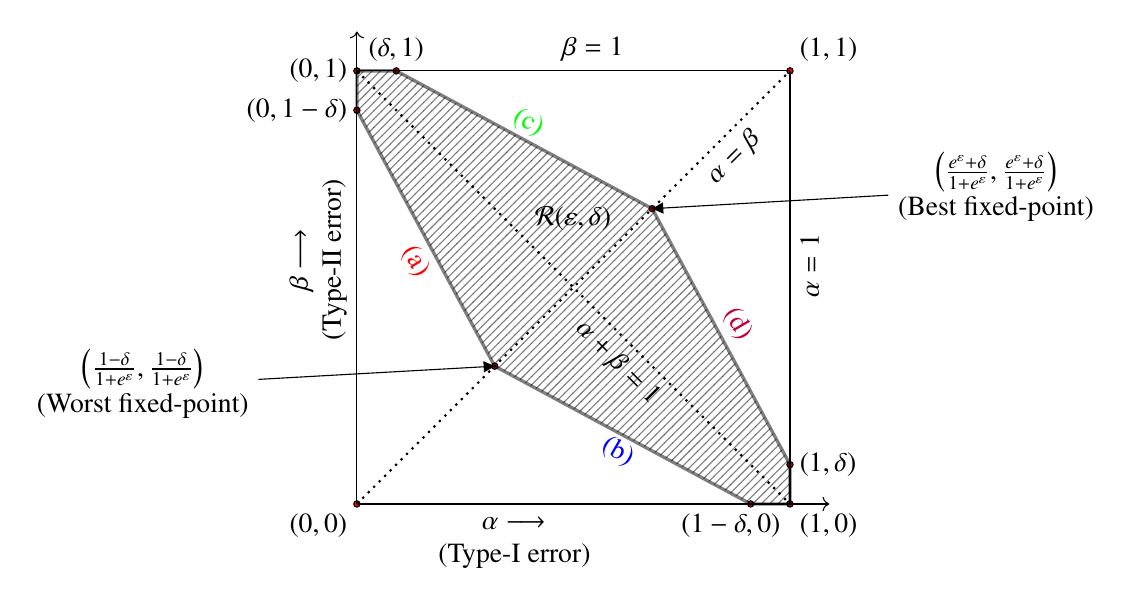
\begin{tikzpicture}

\coordinate (A) at (1.75,1.75);
\coordinate (B) at (0,5);
\coordinate (C) at (0,5.5);
\coordinate (D) at (0.5,5.5);
\coordinate (E) at (3.75,3.75);
\coordinate (F) at (5.5,0.5);
\coordinate (G) at (5.5,0);
\coordinate (H) at (5,0);

\draw[fill=red] (A) circle (0.04); 
\draw[fill=red] (B) circle (0.04); 
\draw[fill=red] (C) circle (0.04); 
\draw[fill=red] (D) circle (0.04); 
\draw[fill=red] (E) circle (0.04); 
\draw[fill=red] (F) circle (0.04); 
\draw[fill=red] (G) circle (0.04); 
\draw[fill=red] (H) circle (0.04); 
\draw[fill=red] (0,0) circle (0.04); 
\draw[fill=red] (5.5,5.5) circle (0.04); 


\draw[->] (0,0) -- (6,0) node[below,xshift = -4cm,yshift = 0.1cm] {\makecell{$\alpha \longrightarrow$ \\ (Type-I error)}};
\draw[->] (0,0) -- (0,6) node[left, rotate = 90, xshift = -1.75cm, yshift = 0.5cm] {\makecell{$\beta \longrightarrow$ \\ (Type-II error)}};
\draw[dotted,thick] (0,0) -- (5.5,5.5) node[anchor = north east, rotate = 45,xshift = -0.75cm] {$\alpha = \beta$};
\draw[dotted,thick] (0,5.5) -- (5.5,0 ) node[anchor = north east, rotate = -45,xshift = -2cm] {$\alpha + \beta = 1$};
\draw[-] (0,5.5) -- (5.5,5.5) node[above, xshift = -2.5cm] {$\beta = 1$};
\draw[-] (5.5,0) -- (5.5,5.5) node[right, xshift = 0.25cm, yshift = -3cm, rotate = 90] {$\alpha = 1$};
\node[anchor = north east] at (0,0) {$(0,0)$};
\node[anchor =  east] at (0,5.5) {$(0,1)$};
\node[anchor = north west] at (5.5,0) {$(1,0)$};
\node[anchor = south west] at (5.5,5.5) {$(1,1)$};




\filldraw[fill=gray, pattern=north east lines, draw=black, very thick, opacity=0.5] (1.75,1.75) -- (0,5) -- (0,5.5)-- (0.5,5.5) -- (3.75,3.75) -- (5.5, 0.5)-- (5.5,0) -- (5,0)-- cycle;



\node[anchor =  east] at (0, 5) {$(0, 1-\delta)$};
\node[anchor =  north, xshift = -0.25 cm] at (5, 0) {$(1-\delta,0)$};
\node[anchor =  south] at (D) {$(\delta, 1)$};
\node[anchor =  west, xshift = 0 cm] at (F) {$(1,\delta)$};

\node[anchor =  east, xshift = -3 cm, yshift = -0.25 cm] (WFP) at (1.75,1.75) {\makecell{$\left(\frac{1-\delta}{1+e^\eps}, \frac{1-\delta}{1+e^\eps}\right)$\\(Worst fixed-point)}};
\node[anchor =  west,xshift=  3cm, yshift = 0.25 cm] (BFP) at (3.75,3.75) {\makecell{$\left(\frac{e^\eps + \delta}{1+e^\eps}, \frac{e^\eps + \delta}{1+e^\eps}\right)$\\(Best fixed-point)}};
\draw[-{Triangle[width=4pt,length=4pt]}] (WFP) -- (A);
\draw[-{Triangle[width=4pt,length=4pt]}] (BFP) -- (E);

\node[anchor = east,xshift = -0.1cm, rotate = -60] at (1,2.8) {\textcolor{red}{(a)}};
\node[anchor = east,xshift = 0.8cm, yshift = -0.5cm, rotate = -30] at (2.8,1) {\textcolor{blue}{(b)}};
\node[anchor = west,xshift = -0.1cm, rotate = -30] at (2,5) {\textcolor{green}{(c)}};

\node[anchor = south,yshift = 0.6cm] at (2.75,2.75) {$\cR(\eps,\delta)$};

\node[anchor = east,xshift = -0cm, rotate = -60] at (5,2) {\textcolor{purple}{(d)}};

\end{tikzpicture}
    \caption{Graphical representation of  $\cR(\eps,\delta)$ : characteristic region of $(\eps,\delta)$-QDP (in shaded region), where we define the boundaries  \textcolor{red}{(a)}, \textcolor{blue}{(b)}, \textcolor{green}{(c)} and \textcolor{purple}{(d)} to be $\beta = 1- \delta - e^\eps \alpha$, $\beta = e^{-\eps} (1-\delta-\alpha)$, $\beta = 1 - e^{-\eps}(\alpha - \delta)$ and $\beta = e^\eps(1-\alpha) + \delta$ respectively and $\cR(\eps,\delta)$ has two fixed points $(\frac{1-\delta}{1+e^\eps},\frac{1-\delta}{1+e^\eps})$ and $(\frac{e^\eps + \delta}{1+e^\eps}, \frac{e^\eps + \delta}{1+e^\eps})$ as its extremal points, where the former and the latter points are known to be the worst and the best fixed points respectively from the perspective of privacy.}
    \label{fig:privacy_region}
\end{figure}
In Figure \ref{fig:privacy_region}, we illustrate a graphical representation of the characteristic region $\cR(\eps,\delta)$ of $(\eps,\delta)$-QDP.

Therefore, under the constraints mentioned in \cref{char_region_eq1,char_region_eq2,char_region_eq3,char_region_eq4}, we define the characteristic (or operating) region of quantum $(\eps,\delta)$-QDP as follows,

\begin{definition}[Characteristic region of $(\eps,\delta)$-QDP]\label{def_DP_char}
    for some fixed $\eps \geq 0$ and $\delta \in [0,1]$, we define the characteristic region of $(\eps,\delta)$-DP as follows,

    \begin{equation}
        \cR(\eps,\delta) := \left\{(\alpha,\beta) \in [0,1]^2 : ~~\begin{split}
            \beta &\geq e^{-\eps}(1-\delta -\alpha),\\
        \beta &\geq 1 -\delta - e^{\eps}\alpha,\\
        \beta &\leq 1 - e^{-\eps}(\alpha - \delta),\\
        \beta &\leq e^{\eps}(1- \alpha) + \delta.
        \end{split}\right\}.
    \end{equation}
\end{definition}



In Figure \ref{fig:privacy_region} above, we illustrate a graphical representation of the characteristic region of $(\eps,\delta)$-DP. In \cite{KOV15}, the authors studied a characteristic region for classical $(\eps,\delta)$-DP. However, they only considered the region below $\alpha + \beta=1$. This is because, in Figure \ref{fig:privacy_region}, the characteristic region  $\cR(\eps,\delta)$ is symmetric over the straight line $\alpha + \beta=1$. Hirche et al. in \cite{HRF23} plotted $ \cR(\eps,\delta)$ for certain values of $\eps, \delta$.

From \cref{char_region_eq1,char_region_eq2,char_region_eq3,char_region_eq4}, it is trivial to see that for any pair of quantum states $(\rho,\sigma) \in \mathfrak{D}_{(\eps,\delta)}$ (for some fixed $\eps \geq 0$ and $\delta \in [0,1]$), we have $\cR(\rho,\sigma) \subseteq \cR(\eps,\delta)$. 
Moreover, the characteristic region $\cR(\eps,\delta)$ is a convex set. This is because for any two positive operators $0 \preceq \Lambda_1, \Lambda_2 \preceq \bbI$, for any $\theta \in [0,1]$, the operator $\Lambda = \theta \Lambda_1 + (1-\theta) \Lambda_2$ is also a positive operator satisfying $0 \preceq \Lambda \preceq \bbI$. Therefore, it can be verified that $\alpha _\Lambda = \theta \alpha_{\Lambda_1} + (1-\theta) \alpha_{\Lambda_2}$ and $\beta _{\Lambda} = \theta \beta_{\Lambda_1} + (1-\theta) \beta_{\Lambda_2}$, where $(\alpha_{\Lambda_1},\beta_{\Lambda_1})$ and  $(\alpha_{\Lambda_2},\beta_{\Lambda_2})$ belongs to $\cR(\eps,\delta)$. Thus, as $(\alpha_{\Lambda},\beta_{\Lambda})$ also belongs to $\cR(\eps,\delta)$, this implies that $\cR(\eps,\delta)$ is convex. Further, $\cR(\eps,\delta)$ is also a closed set. We will prove this by constructing a pair $(\rho_{(\eps,\delta)},\sigma_{(\eps,\delta)}) \in \mathfrak{D_{(\eps,\delta)}}$, which achieves all the corner points of $\cR(\eps,\delta)$, as mentioned in Figure \ref{fig:privacy_region} above.

Further observe that, in Figure \ref{fig:privacy_region}, $\cR(\eps,\delta)$ has two fixed points (points where $\alpha = \beta$) at $(\frac{1-\delta}{e^\eps+1}, \frac{1-\delta}{e^\eps+1})$ and $(\frac{e^\eps + 
\delta}{e^\eps+1}, \frac{e^\eps +  \delta}{e^\eps+1})$. The former is the worst fixed point and the latter is the best fixed point of $\cR(\eps,\delta)$ from the perspective of privacy. This is because the worst fixed point represents the scenario where the adversary has the most amount of information about the underlying quantum state, i.e., it's least private, while the best fixed point represents the scenario where the attacker has the least information about the underlying quantum state, i.e., it's most private.

The characteristic region $\cR(\eps,\delta)$ also has six more corner/extremal points at $(0,1-\delta)$, $(1-\delta,0)$, $(\delta,1)$, $(1,\delta)$, $(1,\delta)$ and $(\delta,1)$ along with the two fixed points. 
 


In the discussion below, we will give a constructive proof for the existence of a pair of quantum states $(\rho_{(\eps,\delta)},\sigma_{(\eps,\delta)}) \in \mathfrak{D}_{(\eps,\delta)}$ such that $\cR(\rho_{(\eps,\delta)},\sigma_{(\eps,\delta)}) = \cR(\eps,\delta)$ for any given $\eps \geq 0$ and $\delta \in [0,1]$ i.e. we show that for  $(\rho_{(\eps,\delta)},\sigma_{(\eps,\delta)})$, under certain choices of measurements, the pair of type-I ($\alpha$) and type-II errors ($\beta$) achieves the extremal/corner points of $\cR(\eps,\delta)$.

Consider a pair $\rho_{(\eps,\delta)}$ and $\sigma_{(\eps,\delta)}$ over a finite-dimensional Hilbert space $\cH$ such that for a one-dimensional projector $\ketbra{v}$, 

\begin{align}
    \tr[\ketbra{v}\rho_{(\eps,\delta)}] &\triangleq \delta, \label{vketrho}\\
    \tr[\ketbra{v}\sigma_{(\eps,\delta)}] &\triangleq 0.\label{vketsig}
\end{align}


Then, the pair $(\rho_{(\eps,\delta)},\sigma_{(\eps,\delta)})$ achieves the corner point $(\delta,1)$ of $\cR(\eps,\delta)$. 
Similarly, for the one-dimensional projector $\bbI - \ketbra{v}$, the pair $(\rho_{(\eps,\delta)},\sigma_{(\eps,\delta)})$ achieves the corner point $(1-\delta,0)$ of $\cR(\eps,\delta)$.

Further, consider another one-dimensional projector $\ketbra{x}$ which is perpendicular to $\ketbra{v}$, such that,

\begin{align}
    \tr[\ketbra{x}\rho_{(\eps,\delta)}] \triangleq 0, \label{xketrho}\\
    \tr[\ketbra{x}\sigma_{(\eps,\delta)}] \triangleq \delta.\label{xketsig}
\end{align}

Then, the pair $(\rho_{(\eps,\delta)},\sigma_{(\eps,\delta)})$ achieves the corner point $(0,1-\delta)$ of $\cR(\eps,\delta)$.
Similarly, for the one-dimensional projector $\bbI - \ketbra{x}$, the pair $(\rho_{(\eps,\delta)},\sigma_{(\eps,\delta)})$ achieves the corner point $(1,\delta)$ of $\cR(\eps,\delta)$. 


Now, we notice that the cardinality of the support of the state pair $(\rho_{(\eps,\delta)},\sigma_{(\eps,\delta)})$ must be at least $3$, since we need two more corner points to be achieved.

Thus, we consider another one-dimensional projector $\bbI - \ketbra{v} - \ketbra{x}$ which is perpendicular to both $\ketbra{v}$ and $\ketbra{x}$. Therefore, from the above discussions, we have,

\begin{align}
    \tr[\left(\bbI - \ketbra{v} - \ketbra{x}\right)\rho_{(\eps,\delta)}] &= 1-\delta, \label{xvcketrho}\\
    \tr[\left(\bbI - \ketbra{v} - \ketbra{x}\right)\sigma_{(\eps,\delta)}] &= 1 - \delta.\label{xvcketsig}
\end{align}


Thus, the pair $(\rho_{(\eps,\delta)},\sigma_{(\eps,\delta)})$ achieves the point $(1-\delta,\delta)$ of $\cR(\eps,\delta)$. However, this is an interior point of $\cR(\eps,\delta)$ and not a corner point. Thus, it can be easily verified that combining the above one-dimensional projectors, we can never achieve the two fixed points of $\cR(\eps,\delta)$. 
Therefore, we consider the support of the state pair $(\rho_{(\eps,\delta)},\sigma_{(\eps,\delta)})$ to be at least $4$.

We now consider another one-dimensional projector $\ketbra{y}$ which is perpendicular to both $\ketbra{v}$ and $\ketbra{x}$, and we consider the two-dimensional projector $(\ketbra{v} + \ketbra{y})$. For this projector, we have two choices: we can either choose it to achieve the worst fixed point, i.e., $(\frac{1-\delta}{1+e^\eps},\frac{1-\delta}{1+e^\eps})$ or the best fixed point, i.e., $(\frac{e^\eps + \delta}{1+e^\eps}, \frac{e^\eps + \delta}{1+e^\eps})$. We will see that the former choice will lead us to some construction of the pair of quantum states, which achieves all the corner points of $\cR(\eps,\delta)$ but fails to satisfy $(\eps,\delta)$-DP condition. See Remark \ref{remark_worst_choice} below for more details. Thus, we choose the two-dimensional projector $(\ketbra{v} + \ketbra{y})$ to achieve the best fixed point. Towards this, we assume that

\begin{align}
    \tr[(\ketbra{v} + \ketbra{y})\rho_{(\eps,\delta)}] &\triangleq \frac{e^\eps+\delta}{1+e^\eps}, \label{vyketrho}\\
    \tr[\left(\bbI - (\ketbra{v} + \ketbra{y})\right)\sigma_{(\eps,\delta)}] &\triangleq \frac{e^\eps+\delta}{1+e^\eps}.\label{vyketsig}
\end{align} 

Thus, the pair $(\rho_{(\eps,\delta)},\sigma_{(\eps,\delta)})$ achieves the best fixed point $(\frac{e^\eps + \delta}{1+e^\eps}, \frac{e^\eps + \delta}{1+e^\eps})$ of $\cR(\eps,\delta)$ with the help of the two-dimensional projector $\ketbra{v} + \ketbra{y}$.

Now \cref{vketrho,vketsig,vyketrho,vyketsig} gives us,

\begin{align}
    \tr[\ketbra{y}\rho_{(\eps,\delta)}] &= \frac{e^\eps(1-\delta)}{1+e^\eps}, \label{yketrho}\\
\tr[\ketbra{y}\sigma_{(\eps,\delta)}] &= \frac{1-\delta}{1+e^\eps}.\label{yketsig}
\end{align}

Finally, consider the one-dimensional projector $\ketbra{z} = \bbI - \ketbra{v} - \ketbra{x} - \ketbra{y}$ which is perpendicular to $\ketbra{v}$, $\ketbra{x}$ and $\ketbra{y}$. Then, from \cref{vketrho,vketsig,xketrho,xketsig,yketrho,yketsig} we have,

\begin{align}
    \tr[\ketbra{z}\rho_{(\eps,\delta)}] &= \frac{1-\delta}{1+e^\eps}, \label{zketrho}\\
\tr[\ketbra{z}\sigma_{(\eps,\delta)}] &= \frac{e^\eps(1-\delta)}{1+e^\eps}.\label{zketsig}
\end{align}


Thus, one can verify that the pair $(\rho_{(\eps,\delta)},\sigma_{(\eps,\delta)})$ achieves the point $(\frac{1-\delta}{1+e^\eps},\frac{1-\delta}{1+e^\eps})$ of $\cR(\eps,\delta)$ with the help of the two-dimensional projector $\ketbra{x} + \ketbra{z}$.

Therefore, we have constructed a pair of quantum states $(\rho_{(\eps,\delta)},\sigma_{(\eps,\delta)})$ which can be written as follows,
\begin{align}
    \rho_{(\eps,\delta)} & = \delta \ketbra{v} + \frac{e^\eps(1-\delta)}{1+e^\eps} \ketbra{y} + \frac{1-\delta}{1+e^\eps} \ketbra{z} + 0 \ketbra{x},\label{eq_rho} \\
    \sigma_{(\eps,\delta)} & = 0 \ketbra{v}+ \frac{1-\delta}{1+e^\eps} \ketbra{y} + \frac{e^\eps(1-\delta)}{1+e^\eps} \ketbra{z} + \delta \ketbra{x}.\label{eq_sigma}
\end{align}

Further, one can verify that the pair of quantum states $(\rho_{(\eps,\delta)},\sigma_{(\eps,\delta)}) \in \mathfrak{D}_{(\eps,\delta)}$ where $\rho_{(\eps,\delta)}$ and $\sigma_{(\eps,\delta)}$ are defined in \eqref{eq_rho} and \eqref{eq_sigma} and satisfies all the corner points of $\cR(\eps,\delta)$. 
Hence, we have $\cR(\rho_{(\eps,\delta)},\sigma_{(\eps,\delta)}) = \cR(\eps,\delta)$. Thus, from the existence of $(\rho_{(\eps,\delta)},\sigma_{(\eps,\delta)})$ and the convexity, we observe that $\cR(\eps,\delta)$ is a closed convex set.

To simplify the definition of $\rho_{(\eps,\delta)}$ and $\sigma_{(\eps,\delta)}$, we consider the Hilbert space $\cH$ to be four-dimensional with the orthonormal basis $\{\ket{00},\ket{01},\ket{10},\ket{11}\}$. Thus, we can rewrite $\rho_{(\eps,\delta)}$ and $\sigma_{(\eps,\delta)}$ as follows,
\begin{align}
    \rho_{(\eps,\delta)} & = \delta \ketbra{00} + (1-\delta)\left(\frac{e^\eps}{1+e^\eps} \ketbra{01} + \frac{1}{1+e^\eps} \ketbra{10}\right),\label{eq_rho_simp}\\
    \sigma_{(\eps,\delta)} & =  (1-\delta)\left(\frac{1}{1+e^\eps} \ketbra{01} + \frac{e^\eps}{1+e^\eps} \ketbra{10}\right) + \delta \ketbra{11}.\label{eq_sigma_simp}
\end{align}

\begin{figure}[h]
    \centering
    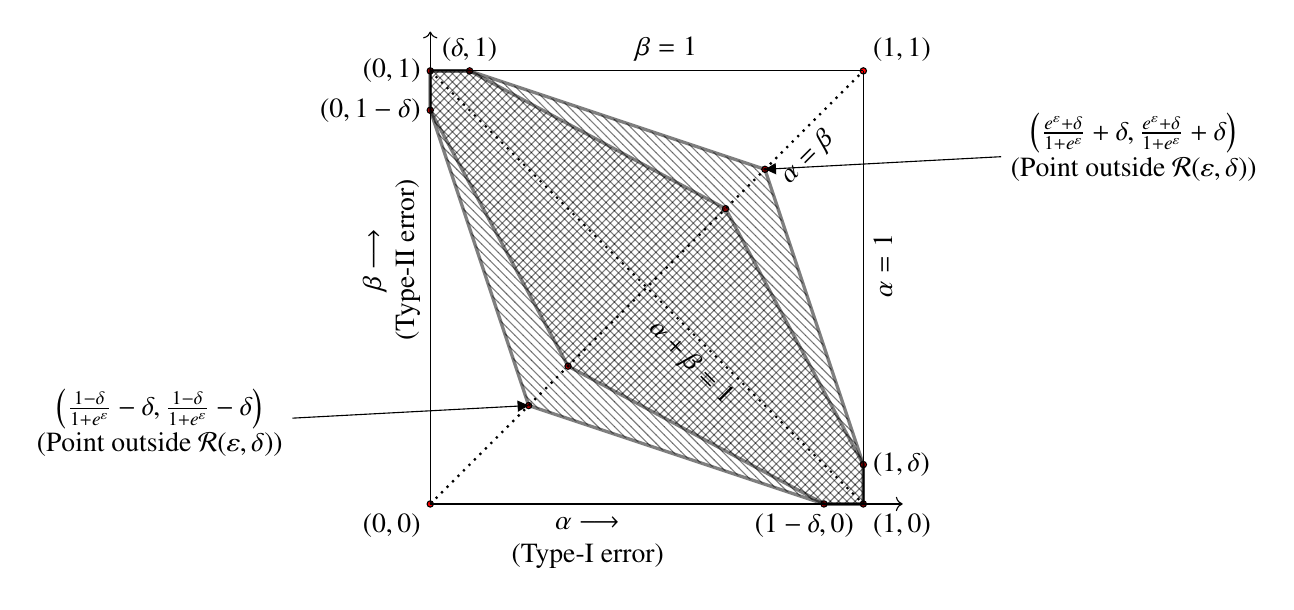
\begin{tikzpicture}

\coordinate (A) at (1.75,1.75);
\coordinate (B) at (0,5);
\coordinate (C) at (0,5.5);
\coordinate (D) at (0.5,5.5);
\coordinate (E) at (3.75,3.75);
\coordinate (F) at (5.5,0.5);
\coordinate (G) at (5.5,0);
\coordinate (H) at (5,0);
\coordinate (I) at (1.25,1.25);
\coordinate (J) at (4.25,4.25);

\draw[fill=red] (A) circle (0.04); 
\draw[fill=red] (B) circle (0.04); 
\draw[fill=red] (C) circle (0.04); 
\draw[fill=red] (D) circle (0.04); 
\draw[fill=red] (E) circle (0.04); 
\draw[fill=red] (F) circle (0.04); 
\draw[fill=red] (G) circle (0.04); 
\draw[fill=red] (H) circle (0.04); 
\draw[fill=red] (I) circle (0.04);
\draw[fill=red] (J) circle (0.04);
\draw[fill=red] (0,0) circle (0.04); 
\draw[fill=red] (5.5,5.5) circle (0.04); 


\draw[->] (0,0) -- (6,0) node[below,xshift = -4cm,yshift = 0.1cm] {\makecell{$\alpha \longrightarrow$ \\ (Type-I error)}};
\draw[->] (0,0) -- (0,6) node[left, rotate = 90, xshift = -1.75cm, yshift = 0.5cm] {\makecell{$\beta \longrightarrow$ \\ (Type-II error)}};
\draw[dotted,thick] (0,0) -- (5.5,5.5) node[anchor = north east, rotate = 45,xshift = -0.75cm] {$\alpha = \beta$};
\draw[dotted,thick] (0,5.5) -- (5.5,0 ) node[anchor = north east, rotate = -45,xshift = -2cm] {$\alpha + \beta = 1$};
\draw[-] (0,5.5) -- (5.5,5.5) node[above, xshift = -2.5cm] {$\beta = 1$};
\draw[-] (5.5,0) -- (5.5,5.5) node[right, xshift = 0.25cm, yshift = -3cm, rotate = 90] {$\alpha = 1$};
\node[anchor = north east] at (0,0) {$(0,0)$};
\node[anchor =  east] at (0,5.5) {$(0,1)$};
\node[anchor = north west] at (5.5,0) {$(1,0)$};
\node[anchor = south west] at (5.5,5.5) {$(1,1)$};




\filldraw[fill=red, pattern=north east lines, draw=black, very thick, opacity=0.5] (1.75,1.75) -- (0,5) -- (0,5.5)-- (0.5,5.5) -- (3.75,3.75) -- (5.5, 0.5)-- (5.5,0) -- (5,0)-- cycle;
\filldraw[fill= blue, pattern=north west lines, draw=black, very thick, opacity=0.5] (I) -- (0,5) -- (0,5.5)-- (0.5,5.5) -- (J) -- (5.5, 0.5)-- (5.5,0) -- (5,0)-- cycle;



\node[anchor =  east] at (0, 5) {$(0, 1-\delta)$};
\node[anchor =  north, xshift = -0.25 cm] at (5, 0) {$(1-\delta,0)$};
\node[anchor =  south] at (D) {$(\delta, 1)$};
\node[anchor =  west, xshift = 0 cm] at (F) {$(1,\delta)$};

\node[anchor =  east, xshift = -3 cm, yshift = -0.25 cm] (WFP) at (I) {\makecell{$\left(\frac{1 -\delta}{1+e^\eps} - \delta,\frac{1 -\delta}{1+e^\eps} - \delta\right)$ \\ (Point outside $\cR(\eps,\delta)$)}};
\node[anchor =  west,xshift=  3cm, yshift = 0.25 cm] (BFP) at (J) {\makecell{$\left(\frac{e^\eps+\delta}{1 + e^\eps} +\delta, \frac{e^\eps+\delta}{1 + e^\eps} +\delta\right)$\\(Point outside $\cR(\eps,\delta)$)}};
\draw[-{Triangle[width=4pt,length=4pt]}] (WFP) -- (I);
\draw[-{Triangle[width=4pt,length=4pt]}] (BFP) -- (J);


\end{tikzpicture}
    \caption{Graphical representation of  $\cR(\rho'_{(\eps,\delta)},\sigma'_{(\eps,\delta)} )$ (in the whole shaded region) which is strictly larger than $\cR(\eps,\delta)$ (in inner shaded region), where the two extremal points of $\cR(\rho'_{(\eps,\delta)},\sigma'_{(\eps,\delta)} )$ outside $\cR(\eps,\delta)$ are $\left(\frac{1 -\delta}{1+e^\eps} - \delta,\frac{1 -\delta}{1+e^\eps} - \delta\right)$ and $\left(\frac{e^\eps+\delta}{1 + e^\eps} +\delta, \frac{e^\eps+\delta}{1 + e^\eps} +\delta\right)$.}
    \label{fig:privacy_region_invalid}
\end{figure}





\begin{remark}\label{remark_worst_choice}
\begin{itemize}
    \item[] ~
    \item It is important to note that in \eqref{vyketrho} and \eqref{vyketsig}, if we had chosen the RHS to be $\frac{1-\delta}{1+e^\eps}$ and $\frac{1-\delta}{1+e^\eps}$ respectively, we would get another pair of quantum states $(\rho'_{(\eps,\delta)},\sigma'_{(\eps,\delta)})$ which also achieves the extremal points of the characteristic region $\cR(\eps,\delta)$ for any given $\eps \geq 0$ and $\delta \in [0,1]$. This pair is given as follows,
    \begin{align}
        \rho'_{(\eps,\delta)} & = \delta \ketbra{00} + \frac{1-2\delta-e^\eps\delta}{1+e^\eps} \ketbra{01} + \frac{e^\eps + \delta}{1+e^\eps} \ketbra{10},\label{eq_rho'_simp}\\
        \sigma'_{(\eps,\delta)} & =  \frac{e^\eps + \delta}{1+e^\eps} \ketbra{01} + \frac{1-2\delta-e^\eps\delta}{1+e^\eps} \ketbra{10} + \delta \ketbra{11}.\label{eq_sigma'_simp}
    \end{align}
    However, the pair  $(\rho'_{(\eps,\delta)},\sigma'_{(\eps,\delta)})$ also achieves two points $\left(\frac{1 -\delta}{1+e^\eps} - \delta,\frac{1 -\delta}{1+e^\eps} - \delta\right)$ and $\left(\frac{e^\eps+\delta}{1 + e^\eps} +\delta, \frac{e^\eps+\delta}{1 + e^\eps} +\delta\right)$, which are outside the characteristic region $\cR(\eps,\delta)$. From this, we can conclude that the pair $(\rho'_{(\eps,\delta)},\sigma'_{(\eps,\delta)}) \not\in \mathfrak{D}_{(\eps,\delta)}$.
    \item Further, one can verify that the above pair satisfies $(\log (\frac{e^\eps}{1 - \delta(2 + e^\eps)}),\delta)$-DP.

\end{itemize}    
\end{remark}

In Figure \ref{fig:privacy_region_invalid} above, we illustrate a graphical representation of the characteristic region $\cR(\rho'_{(\eps,\delta)},\sigma'_{(\eps,\delta)} )$ along with the extremal points achieved by the pair $(\rho'_{(\eps,\delta)},\sigma'_{(\eps,\delta)})$.

\begin{remark}
    In \cite{BG17}, the authors obtained a figure similar to Figure \ref{fig:privacy_region} by plotting type-1 and type-2 errors for a pair of states $\{\rho_1,\rho_2\}$. In contrast, Figure \ref{fig:privacy_region} is with respect to all pairs $\{\rho_1,\rho_2\}$ which are $(\eps,\delta)$-DP and therefore it helps to characterize the worst-case (most informative) $(\eps,\delta)$-DP pair of quantum states.
\end{remark}


\section{Quantum Information Ordering and Differential Privacy}\label{sec_diff_priv_quant}

\subsection{Quantum ordering of informativeness}

In \cite{Blackwell51,BG54}, Blackwell introduced a notion of an ordering of classical informativeness between two pairs of distributions $\{P_1,P_2\}$ and $\{Q_1,Q_2\}$. In particular, he proved the following proposition,

\begin{proposition}[Blackwell's Theorem of Informativeness Ordering {\cite[Theorems $12.2.2$ \& $12.4.2$]{BG54}}]\label{prop_blackwell}
    Given two pairs of probability distributions $\left(P_1,P_2\right)$ and $\left(Q_1,Q_2\right)$ over two finite sets $\cX$ and $\cY$, respectively, the following statements are equivalent,
    \begin{enumerate}
        \item $\left\{P_1,P_2\right\} \succeq_{B} \left\{Q_1,Q_2\right\}$.
        \item $D^{\alpha}_{H}{(P_1\|P_2)} \geq D^{\alpha}_{H}{(Q_1\|Q_2)} $ for all $\alpha \in [0,1]$, where $D^{\alpha}_{H}{(P_1\|P_2)}$ and $D^{\alpha}_{H}{(Q_1\|Q_2)}$ are the classical hypothesis testing divergence of order $\alpha$ (see Definition \ref{def_hyp_div}) between the pair of distributions $\left\{P_1,P_2\right\}$ and $\left\{Q_1,Q_2\right\}$ respectively.
        \item There exists a stochastic map $\cT : \cX \to \cY$ such that $Q_i = \cT(P_i)$ for each $i \in \{1,2\}$.\label{map_exist}
    \end{enumerate}
\end{proposition}


Analogous to Blackwell's order of classical informativeness (as mentioned in Proposition \ref{prop_blackwell}), we discuss a quantum version of it, which provides an ordering of quantum statistical experiments based on their distinguishability. Using the quantum hypothesis testing divergence as the underlying measure, we formalize when one pair of quantum states can be considered more informative than another. We further establish that this dominance relation implies a corresponding ordering across all quantum $f$-divergences, thereby linking hypothesis testing quantities to a broad class of information-theoretic measures.

We now make the following definition.

\begin{definition}[Quantum information  order]\label{def_quant_blackwell}
    Consider two pairs of quantum states $(\rho_1,\rho_2)$ and  $(\sigma_1,\sigma_2)$. We say that the pair $\left(\rho_1,\rho_2\right)$ dominates (or, is more informative than) the  pair $\left(\sigma_1,\sigma_2\right)$ (denoted as $\left\{\rho_1,\rho_2\right\} \succeq_{Q} \left\{\sigma_1,\sigma_2\right\}$), if for all $\alpha \in [0,1]$, the following holds,
    \begin{equation}
        D^{\alpha}_{H}{(\rho_1\|\rho_2)} \geq D^{\alpha}_{H}{(\sigma_1\|\sigma_2)}.\label{def_quant_blackwell_eq}
    \end{equation}
\end{definition}

 Intuitively, the order $\left\{\rho_1,\rho_2\right\} \succeq_{Q} \left\{\sigma_1,\sigma_2\right\}$ indicates that the states $\rho_1$ and $\rho_2$ are more distinguishable as compared to the states $\sigma_1$ and $\sigma_2$. 

Unlike the classical case, in the quantum setting, from the results of \cite{Matsumoto2014} and  of \cite[Lemma $18$ \& Corollary $19$]{GLW24}, it is known that \eqref{def_quant_blackwell_eq} \textit{does not} always imply the existence of a CP-TP map $\cE$ such that $\sigma_i = \cE(\rho_i)$ for each $i \in \{1,2\}$. This yields that we \textit{can not} invoke the monotonicity property of quantum divergences (see Definition \ref{def_data_proc_func}) to conclude that $\varmathbb{D}(\rho_1\| \rho_2) \geq \varmathbb{D}(\sigma_1\| \sigma_2)$.

However, we can circumvent this issue by directly showing that if for any two pairs of quantum states  $(\rho_1,\rho_2)$ and $(\sigma_1,\sigma_2)$, \eqref{def_quant_blackwell_eq} holds, then, every quantum $f$-divergence (see Definition \ref{def_f_div_integral_rep}) between the former pair dominates that of the latter pair. We formalize this claim in the Theorem below.


 \begin{theorem}\label{lemma_t_hyp_F_Div}
    Consider two pairs of quantum states  $(\rho_1,\rho_2)$ and $(\sigma_1,\sigma_2)$, for which the following holds,

\begin{equation}
    D^{\alpha}_{H}{(\rho_1\|\rho_2)} \geq D^{\alpha}_{H}{(\sigma_1\|\sigma_2)}, \forall \alpha \in [0,1].\label{lemma_t_hyp_F_div_eq}
\end{equation}

Then, for any $f \in \cF$ (see Definition \ref{def_f_div_integral_rep}) we have, 
$$D_f(\rho_1\|\rho_2) \geq  D_f(\sigma_1\|\sigma_2),$$ whenever $D_f$ is well-defined (see Definition \ref{def_f_div_integral_rep}) for the pairs $(\rho_1,\rho_2)$ and $(\sigma_1,\sigma_2)$.
\end{theorem}

    Before proceeding with the proof of Theorem \ref{lemma_t_hyp_F_Div}, we first state the following lemma, which will be required in proving Theorem \ref{lemma_t_hyp_F_Div}.
    \begin{lemma}\label{fact_equi_ah_sd}
        Consider $\rho_1,\rho_2 \in \cD(\cH_A)$ and $\sigma_1,\sigma_2 \in \cD(\cH_B)$. If
        \begin{equation}
            D^{\alpha}_{H}{(\rho_1\|\rho_2)} \geq D^{\alpha}_{H}{(\sigma_1\|\sigma_2)}, \forall \alpha \in [0,1],\label{fact_equi_ah_sd_eq}
        \end{equation}
        then,
\begin{align}
            E_{\gamma}(\rho_1\|\rho_2) &\geq E_{\gamma}(\sigma_1\|\sigma_2), \forall \gamma\geq 0, \label{BN1}\\
            D_{\tilde{\alpha}}(\rho_1\|\rho_2) &\geq D_{\tilde{\alpha}}(\sigma_1\|\sigma_2), \forall 
            \tilde{\alpha} \in [0,1) \cup (1,+\infty),\label{BN2} \\
            D(\rho_1\|\rho_2) &\geq D(\sigma_1\|\sigma_2),\label{BN2B}
        \end{align}
        where $E_{\gamma} (\cdot \|\cdot)$ 
        and $D_{\tilde{\alpha}}(\cdot \|\cdot)$
        are defined in Definitions \ref{f_sym_hyp_func} and \ref{def_quant_renyi_hockey}.
    \end{lemma}
    \begin{proof}
        See Appendix \ref{proof_fact_equi_ah_sd} for the proof.
    \end{proof}
    Using the above lemma, we now prove Theorem \ref{lemma_t_hyp_F_Div} using the following series of inequalities,
    \begin{align*}
        D_{f}(\rho_1\|\rho_2) &\overset{(a)}{=} \int_{0}^{\infty} f''(\gamma) E_{\gamma}(\rho_1\|\rho_2) d\gamma\nn\\
        &\overset{(b)}{\geq} \int_{0}^{\infty} f''(\gamma) E_{\gamma}(\sigma_1\|\sigma_2) d\gamma\nn\\
        &\overset{(c)}{=} D_{f}(\sigma_1\|\sigma_2),
    \end{align*}
    where $(a)$ and $(c)$ follows from Fact \ref{fact_f_div_integral_rep} and $(b)$ follows from \eqref{BN1} of Lemma \ref{fact_equi_ah_sd} and the fact that the double derivative of $f$ exists and $f$ is a convex function. This completes the proof of Theorem \ref{lemma_t_hyp_F_Div}. 


\begin{remark}
    We note here that \eqref{BN1} of Lemma \ref{fact_equi_ah_sd} was also proven in \cite[Theorem $2$]{BG17}.
\end{remark}

\begin{remark}
    There have been various notions of ordering of informativeness in the quantum case in the earlier works, see for example,  \cite{ReebKastoryanoWolf2011,Buscemi2012,Jencova2012,Matsumoto:2015vgh,Buscemi2016,Buscemi_2018,BuscemiSutterTomamichel2019,WW19}. However, it is not very clear whether these orderings are useful for characterizing differentially private mechanisms, which is the main aim of this manuscript.
\end{remark}

\subsection{Differential privacy: A quantum hypothesis testing perspective}

In this subsection, we consider differential privacy from a quantum hypothesis testing perspective. The main goal of quantum differential privacy is to ensure that a quantum mechanism produces output states that are nearly indistinguishable when applied to neighboring quantum inputs. Formally, for two neighboring quantum inputs producing output states $\rho, \sigma$, the distinguishability between $\rho$ and $\sigma$ must be limited by the privacy parameters. Intuitively, this means that even if an investigator (adversary) knows the mechanism and observes its output, the investigator should not be able to reliably infer which quantum input (respondent) generated it. More formally, with high probability, no hypothesis test—regardless of the investigator’s strategy—can reliably infer the respondent’s individual contribution from the output.

Motivated by the close relation between privacy and hypothesis testing, in the lemma below, we give an equivalent condition for a pair of quantum states to be $(\eps,\delta)$-DP (see Definition \ref{def_DP_state}). 


\begin{lemma}\label{lemma_DP_t_hyp_rel}
    Consider any pair of quantum states $(\rho,\sigma) \in \mathfrak{D}_{(\eps,\delta)} $ (see Definition \ref{def_DP_state}) for some fixed $\eps \geq 0$ and $\delta \in [0,1)$. Then, the following holds,
\begin{equation}
    D^{\alpha}_{H} {(\rho\|\sigma)} \leq -\log f_{\eps,\delta}(\alpha), \forall \alpha \in [0,1], \label{lemma_DP_t_hyp_rel_eq}
\end{equation}
or, equivalently,
\begin{equation}
    \beta(\alpha|\rho\|\sigma) \geq  f_{\eps,\delta}(\alpha), \forall \alpha \in [0,1], \label{lemma_DP_t_hyp_rel_eq1}
\end{equation}
where,
\begin{equation}
    f_{\eps,\delta}(\alpha) := \max\left\{1 - \delta - e^{\eps}\alpha, e^{-\eps}(1 -\delta-\alpha),0\right\},\label{fepdel}
\end{equation}
 for any $\alpha \in [0,1]$.
\end{lemma}

\begin{proof}
    See Appendix \ref{proof_lemma_DP_t_hyp_rel} for the proof.
\end{proof}



Note that the above version of quantum $(\eps,\delta)$-DP implies that if for each $\alpha \in [0,1]$ $D^{\alpha}_H(\rho'\|\sigma') =-\log f_{\eps,\delta}(\alpha)$ for some pair of quantum states $\rho',\sigma'$ over any arbitrary finite dimensional Hilbert space, then for any pair of quantum states $\rho,\sigma \in \mathfrak{D}_{(\eps,\delta)}$ (see Definition \ref{def_DP_state}) is at least as hard as distinguishing between the pair $(\rho',\sigma')$.
The above intuition provides a notion of the weakest (most informative) quantum $(\eps,\delta)$-DP pairs of quantum states, which are the least ``hard to differentiate''. We formalize this notion in the definition below.

\begin{definition}[Weakest quantum $(\eps,\delta)$-DP]\label{def_opt_DP_state}
     For $\eps \geq 0 $ and $\delta \in [0,1),$ a pair of quantum states $(\rho,\sigma)$ is defined to be the weakest (most informative) quantum $(\eps,\delta)$-DP if
\begin{equation}
    D^{\alpha}_{H} {(\rho\|\sigma)} = -\log f_{\eps,\delta}(\alpha), \forall \alpha \in [0,1], \label{def_opt_DP_state_eq}
\end{equation}
\end{definition}

In the lemma below, we show the existence of a pair of quantum states that is the weakest (most informative) quantum $(\eps,\delta)$-DP (see Definition \ref{def_opt_DP_state}) for some fixed $\eps \geq 0$ and $\delta \in [0,1]$.

\begin{lemma}\label{lemma_diff_priv_quant}
    Consider the quantum states $\rho_{(\eps,\delta)}$ and $\sigma_{(\eps,\delta)}$ mentioned in \eqref{eq_rho_simp} and \eqref{eq_sigma_simp}, for some fixed $\eps \geq 0$ and $\delta \in [0,1]$. 
    Then, we have $D^{\alpha}_{H}(\rho_{(\eps,\delta)}\|\sigma_{(\eps,\delta)}) = -\log f_{\eps,\delta}(\alpha)$ for any $\alpha \in [0,1]$.
\end{lemma}
\begin{proof}
    See Appendix \ref{proof_lemma_diff_priv_quant} for the proof.
\end{proof}

Therefore, for a pair $(\rho,\sigma) \in \mathfrak{D}_{(\varepsilon,\delta)}$ with some fixed $\varepsilon \geq 0$ and $\delta \in [0,1]$,
Lemmas~\ref{lemma_DP_t_hyp_rel} and~\ref{lemma_diff_priv_quant} guarantee the relation,
    \begin{align}
        D^{\alpha}_{H}(\rho\|\sigma) &\leq -\log f_{\eps,\delta}(\alpha)
        = D^{\alpha}_{H}(\rho_{(\eps,\delta)}\|\sigma_{(\eps,\delta)}),\label{theo_QLDP_approx_F_div_eq1}
    \end{align}
 for every $\alpha \in [0,1]$.

 Further, from Lemmas \ref{lemma_DP_t_hyp_rel} and \ref{lemma_diff_priv_quant} and Definition \ref{def_quant_blackwell}, we note that any pair of quantum states $(\rho,\sigma) \in \mathfrak{D}_{(\eps,\delta)}$ for some fixed $\eps \geq 0$ and $\delta \in [0,1]$, gets dominated by the pair $(\rho_{(\eps,\delta)},\sigma_{(\eps,\delta)})$. Formally, it implies the following. 


\begin{corollary}\label{corr_QLDP_blackwell}
    If any pair of quantum states $(\rho,\sigma) \in \mathfrak{D}_{(\eps,\delta)}$ for some fixed $\eps \geq 0$ and $\delta \in [0,1]$, then the following holds,
    \begin{equation}
       \left\{\rho_{(\eps,\delta)},\sigma_{(\eps,\delta)}\right\} \succeq_{Q}  \left\{\rho,\sigma\right\} .\label{corr_QLDP_blackwell_eq}
    \end{equation}
\end{corollary}

\begin{remark}\hfill
   \begin{itemize}
    \item Note that the quantum states $\rho_{(\eps,\delta)}$ and $\sigma_{(\eps,\delta)}$ mentioned in Lemma \ref{lemma_diff_priv_quant}, which satisfies weakest (most informative) $(\eps,\delta)$-DP condition for fixed $\eps \geq 0$ and $\delta \in [0,1]$, has a fixed-point at $\alpha = \frac{1-\delta}{e^\eps+1}$. 
    \item For $\delta = 0$ and any $\eps \geq 0$, we define two quantum states, 
    \begin{align}
        \rho_{(\eps)} &:= \frac{e^\eps}{1+e^\eps}\ketbra{0} + \frac{1}{1+e^\eps}\ketbra{1},\label{rho_pure_weak}\\
        \sigma_{(\eps)} &:= \frac{1}{1+e^\eps}\ketbra{0} + \frac{e^\eps}{1+e^\eps}\ketbra{1},\label{sigma_pure_weak}
    \end{align}
     Observe that it can be verified that $\rho_{(\eps)}$ and $\sigma_{(\eps)}$ are the weakest (most informative) $\eps$-DP pair of quantum states.
   \end{itemize}
\end{remark}

We now state the main theorem of this section, which provides a bound on $D_f(\rho\|\sigma)$ (see Definition \ref{def_f_div_integral_rep}) for any pair of quantum states $(\rho,\sigma) \in \mathfrak{D}_{(\eps,\delta)}$.

\begin{theorem}\label{theo_QLDP_approx_F_div_bound}
    If a pair of quantum states $(\rho,\sigma)$ belongs to $\mathfrak{D}_{(\eps,\delta)}$ for some fixed $\eps \geq 0$ and $\delta \in [0,1]$, 
    then for any $f \in \cF$, we have,
    \begin{equation}
        D_f(\rho\|\sigma) \leq D_f(\rho_{(\eps,\delta)}\|\sigma_{(\eps,\delta)}),\label{theo_QLDP_approx_F_div_eq}
    \end{equation}
    whenever $D_f$ is well-defined for the pairs $(\rho_1,\rho_2)$ and $(\rho_{(\eps,\delta)},\sigma_{(\eps,\delta)})$.
Also, for any $\gamma \geq 0$
    and $\alpha \in [0,1) \cup (1,+\infty)$, we have,
    \begin{align}
        E_{\gamma}(\rho\|\sigma)& \leq E_{\gamma}(\rho_{(\eps,\delta)}\|\sigma_{(\eps,\delta)}),\label{corr_QLDP_approx_hockey_eq} \\
        D_{\alpha}(\rho\|\sigma)& \leq D_{\alpha}(\rho_{(\eps,\delta)}\|\sigma_{(\eps,\delta)}),\label{corr_QLDP_P} \\
        D(\rho\|\sigma)& \leq D(\rho_{(\eps,\delta)}\|\sigma_{(\eps,\delta)}),\label{corr_QLDP_Re} \\
        \check{D}_{\alpha}(\rho\|\sigma)& \leq \check{D}_{\alpha}(\rho_{(\eps,\delta)}\|\sigma_{(\eps,\delta)}).\label{corr_QLDP_S}
    \end{align}
\end{theorem}
\begin{proof}
Suppose a pair $(\rho,\sigma)$ belongs to 
$\mathfrak{D}_{(\varepsilon,\delta)}$ for some fixed $\varepsilon \geq 0$ and $\delta \in [0,1]$. 
   Then, the combination of \eqref{theo_QLDP_approx_F_div_eq1} and
Theorem \ref{lemma_t_hyp_F_Div} implies the relation $D_f(\rho\|\sigma) \leq D_f(\rho_{(\eps,\delta)}\|\sigma_{(\eps,\delta)})$. 
The combination of \eqref{theo_QLDP_approx_F_div_eq1} and
Lemma \ref{fact_equi_ah_sd}
also implies 
\eqref{corr_QLDP_approx_hockey_eq}, \eqref{corr_QLDP_P}, and \eqref{corr_QLDP_Re}.
    Finally, using Fact \ref{fact_P_div_integral_rep}, we have, 
    \begin{align}
            \check{D}_{\alpha}(\rho\|\sigma)\leq 
                    D_{\alpha}(\rho\|\sigma) \leq D_{\alpha}(\rho_{(\eps,\delta)}\|\sigma_{(\eps,\delta)})=
            \check{D}_{\alpha}(\rho_{(\eps,\delta)}\|\sigma_{(\eps,\delta)}),    \end{align}
    where the final equality follows from Fact \ref{fact:commuting_renyi_full}, since 
    $\rho_{(\eps,\delta)}$ and $\sigma_{(\eps,\delta)}$
   are commutative with each other. 
    This proves Theorem \ref{theo_QLDP_approx_F_div_bound}.
\end{proof}


Further, for $\delta =0$, the theorem below gives an upper-bound on $D_f$ (for any $f \in \cF$) between any pair of quantum states $(\rho,\sigma) \in \mathfrak{D}_{(\eps,0)}$.
\begin{corollary}\label{theo_QLDP_F_div_pure_bound}
    If any pair of quantum states $(\rho,\sigma) \in \mathfrak{D}_{(\eps,0)}$ for some fixed $\eps \geq 0$, then for any $f \in \cF$, $\gamma \geq 0$
    and $\alpha \in [0,1) \cup (1,+\infty)$, we have,
    \begin{align}
        D_f(\rho\|\sigma) &\leq D_f(\rho_{(\eps)}\|\sigma_{(\eps)}),\label{theo_QLDP_F_div_pure_bound_eq}\\
        E_{\gamma}(\rho\|\sigma)& \leq E_{\gamma}(\rho_{(\eps)}\|\sigma_{(\eps)}),\label{theo_QLDP_F_div_pure_bound_eq2} \\
        D_{\alpha}(\rho\|\sigma)
        & \leq D_{\alpha}(\rho_{(\eps)}\|\sigma_{(\eps)}),\label{theo_QLDP_F_div_pure_bound_eq3}\\
        \check{D}_{\alpha}(\rho\|\sigma)& \leq 
        \check{D}_{\alpha}(\rho_{(\eps)}\|\sigma_{(\eps)}).\label{theo_QLDP_F_div_pure_bound_eq4}
    \end{align}
   whenever $D_f$ is well-defined for the pairs $(\rho,\sigma)$ and $(\rho_{(\eps)},\sigma_{(\eps)})$ (defined in \eqref{rho_pure_weak} and \eqref{sigma_pure_weak} respectively).
\end{corollary}
\begin{remark}
    Note that for some fixed $\eps \geq 0$, the pair $(\rho_{(\eps)},\sigma_{(\eps)})$ is commutative and $D_{\max}(\rho_{(\eps)}\|\sigma_{(\eps)})= D_{\max}(\sigma_{(\eps)}\|\rho_{(\eps)})$ $ = \eps$. 
    Further, Definition \ref{def_DP_state} directly guarantees that 
     any pair of quantum states $(\rho,\sigma) \in \mathfrak{D}_{(\eps,0)}$ satisfies 
    \begin{align*}
        D_{\max}(\rho\|\sigma) & \leq \eps = D_{\max}(\rho_{(\eps)}\|\sigma_{(\eps)}), \nn\\
        D_{\max}(\sigma\|\rho) &\leq \eps = D_{\max}(\sigma_{(\eps)}\|\rho_{(\eps)}).
            \end{align*}
     Therefore, from Fact \ref{fact_state_trans}, there exists a CP-TP map $\cE$, such that $\rho = \cE(\rho_{(\eps)}) $ and $\sigma =\cE(\sigma_{(\eps)})$. Hence, Definition \ref{def_data_proc_func} implies 
     \begin{equation*}
         \varmathbb{D}(\rho\|\sigma) \leq \varmathbb{D}(\rho_{(\eps)}\|\sigma_{(\eps)}).
     \end{equation*}
\end{remark}



It is important to note that for $\delta > 0$, $\supp(\rho_{(\eps,\delta)}) \not\subseteq \supp(\sigma_{(\eps,\delta)})$. Therefore, the divergence that requires support inclusion is not well-defined for the pair of quantum states $\rho_{(\eps,\delta)}$ and $\sigma_{(\eps,\delta)}$.
Although for the case when $\delta = 0$, since $\supp(\rho_{\eps}) = \supp(\sigma_{\eps})$, for any $\eps$-DP quantum state pairs, using Corollary \ref{theo_QLDP_F_div_pure_bound}, we derive upper-bounds on quantum relative entropy and $L_1$ distance as mentioned in the corollary below.
\begin{corollary}\label{corr_QLDP_Divs_bound}
    If a pair of quantum states $(\rho,\sigma) \in \mathfrak{D}_{(\eps,0)}$ for some fixed $\eps \geq 0$, 
    then, we have the following upper-bounds,

    \begin{enumerate}[label=(\roman*)]
        \item $D(\rho\|\sigma) \leq  \eps \tanh \left(\frac{\eps}{2}\right)$\label{corr_QLDP_KL_bound_eq},
        \vspace*{5pt} 
        \item $\norm{\rho-\sigma}{1} \leq 2 \tanh \left(\frac{\eps}{2}\right)$. \label{corr_QLDP_Hockey_Stick_bound_eq}
    \end{enumerate}
\end{corollary}

\begin{proof}
    \hfill\\
    \emph{(i)} Fact \ref{fact_KL_div_integral_rep} yields that $D(\cdot\|\cdot) = D_{f}(\cdot\|\cdot)$, where $f(x) = x \log x$. 
    Further, the pair $(\rho_{(\eps)},\sigma_{(\eps)})$ satisfies the following,
    \begin{align}
        D(\rho_{(\eps)}\|\sigma_{(\eps)}) &= \frac{e^\eps}{1+e^\eps} \eps - \frac{1}{1+e^\eps}\eps\nn\\
                          &= \eps\left(\frac{e^{\frac{\eps}{2}} - e^{-\frac{\eps}{2}}}{e^{\frac{\eps}{2}} + e^{-\frac{\eps}{2}}}\right)
                          = \eps \tanh\left(\frac{\eps}{2}\right).
    \end{align}

Therefore, \eqref{theo_QLDP_F_div_pure_bound_eq} of Corollary \ref{theo_QLDP_F_div_pure_bound} completes the proof of \emph{(i)} of Corollary \ref{corr_QLDP_Divs_bound}.
 

 
\emph{(ii)} The pair $(\rho_{(\eps)},\sigma_{(\eps)})$ satisfies the following,
    \begin{align}
       \norm{\rho_{(\eps)}-\sigma_{(\eps)}}{1} &= \abs{\frac{e^\eps - 1}{1+ e^\eps}} + \abs{\frac{1 - e^\eps}{1+ e^\eps}}\nn\\
                          &\overset{(a)}{=} 2\abs{\frac{e^\eps - 1}{1+ e^\eps}}
                          = 2 \tanh\left(\frac{\eps}{2}\right).
    \end{align}
where $(a)$ follows from the fact that $e^\eps \geq 1$ as $\eps \geq 0$.
Note that we have $\norm{\rho-\sigma}{1} = 2 \abs{\rho-\sigma}_{+} = 2 E_{1}(\rho\|\sigma)$, where the last equality follows from Fact \ref{Fact_hockey_equiv_form}.
 Therefore, the relation \eqref{theo_QLDP_F_div_pure_bound_eq2} of Corollary \ref{theo_QLDP_F_div_pure_bound} derives that $\norm{\rho-\sigma}{1} = 2E_{1}(\rho\|\sigma) \leq  2E_{1}(\rho_{(\eps)}\|\sigma_{(\eps)}) = \norm{\rho_{(\eps)}-\sigma_{(\eps)}}{1}$. This completes the proof of \emph{(ii)} of Corollary \ref{corr_QLDP_Divs_bound}.    
\end{proof}

\section{Quantum Privatized Parameter Inference}\label{sec:fisher}
\subsection{Problem setting}
We consider a statistical inference problem with $n$ respondents with the privacy setting.
Respondent $i\in\{1,\ldots,n\}$ holds a private bit $X_i\in\{0,1\}$, and the investigator aims to infer a population parameter
$\theta\in[0,1]$ that governs the relative frequency of the two outcomes.
Concretely, since (from the investigator’s perspective) the respondents’ behavior is modeled as random sampling with replacement, the $n$ private bits can be treated as i.i.d.\ draws from a Bernoulli law $p_\theta$ on $\{0,1\}$ with $p_\theta(0)=\theta$ and $p_\theta(1)=1-\theta$.
Equivalently, the investigator treats the collected answers as random sampling with replacement from a population with
composition parameterized by $\theta$, so that $(X_1,\ldots,X_n)$ is (approximately) i.i.d.\ under $p_\theta$.
The key task is to estimate $\theta$ from the $n$ (privatized) responses.

To gather information while protecting privacy, each respondent releases not the raw bit $X_i$ but a quantum system whose
state depends on $X_i$.
Specifically, we fix two quantum states $\rho$ and $\sigma$, and respondent $i$ releases state $\rho$ if $X_i=0$ and state
$\sigma$ if $X_i=1$.
Thus, each response is produced by an encoding map $x\in\{0,1\}\mapsto \rho_x$, where $\rho_0:=\rho$ and
$\rho_1:=\sigma$.
The privacy requirement is imposed at the level of each respondent's released system.
Namely, we require that the pair of possible outputs of an individual respondent, $(\rho,\sigma)$, satisfies
$(\eps,\delta)$-DP in the sense of Definition~\ref{def_DP_state}, i.e.,
$(\rho,\sigma)\in\mathfrak{D}_{(\varepsilon,\delta)}$.

Parametrized states induced by the population model.
Under the Bernoulli model with parameter $\theta$, a single privatized response is described by the mixture
$\rho_\theta := \theta\,\rho + (1-\theta)\,\sigma$ with $\theta\in[0,1]$.
Since the investigator collects $n$ responses, the resulting joint state is modeled as the product state
$\rho_\theta^{\otimes n}$.
This is the quantum analogue of observing $n$ i.i.d.\ privatized samples drawn according to $p_\theta$, where the unknown
parameter $\theta$ controls the mixture proportions between $\rho$ and $\sigma$.

We also define $\rho_{(\eps,\delta),\theta}$ analogously when the respondents encode their information using the weakest/most
informative $(\eps,\delta)$-DP pair $(\rho_{(\eps,\delta)},\sigma_{(\eps,\delta)})$ constructed earlier in the paper.
That is,
$\rho_{(\eps,\delta),\theta} := \theta\,\rho_{(\eps,\delta)} + (1-\theta)\,\sigma_{(\eps,\delta)}$.
This reference pair plays a canonical role in our analysis: since it is the most informative among all $(\eps,\delta)$-DP
pairs, it provides the fundamental benchmark for the maximum inferential power (e.g., hypothesis testing performance and
Fisher information) achievable by any privatized mechanism under the same privacy parameters.

More generally, quantum parameter inference concerns estimating an unknown parameter $\theta$ encoded in a family of states
$\{\rho_\theta\}$, where the encoding is constrained by privacy requirements.
In the present privatized setting, the requirement $(\rho,\sigma)\in\mathfrak{D}_{(\eps,\delta)}$ restricts the
distinguishability of the two single-shot outputs under \emph{any} measurement and hence limits how much information about
$\theta$ can be extracted from $\rho_\theta^{\otimes n}$.
In the following subsections, we quantify this limitation through (i) privatized hypothesis testing and (ii) bounds on the
(SLD) Fisher information under $(\eps,\delta)$-QDP.

\subsection{Hypothesis testing with one respondent}
First, for the theoretical and fundamental analysis, we consider the scenario where the investigator aims to distinguish between two original information sources, $\rho_{\theta_0}$ and $\rho_{\theta_1}$ with $\theta_0 < \theta_1$, only from one observation; however, this scenario is impractical as it addresses only a single respondent.
The performance in this hypothesis testing task is characterized by quantities like the hypothesis testing divergence $D_H^\alpha( \rho_{\theta_0}\|\rho_{\theta_1})$.

\begin{theorem}\label{THJ}
The maximum hypothesis testing divergence under the $(\eps,\delta)$-DP constraint is given by:
\begin{align}
\max_{(\rho,\sigma) \in \mathfrak{D}_{(\eps,\delta)}} D_H^\alpha( \rho_{\theta_1}\|\rho_{\theta_2}) 
= D_H^\alpha( \rho_{(\eps,\delta),\theta_1}\|\rho_{(\eps,\delta),\theta_0}).
\end{align}
This maximum is uniformly attained by the pair $(\rho_{(\eps,\delta)}, \sigma_{(\eps,\delta)})$.
\end{theorem}

\begin{proof}
It is sufficient to show
\begin{align}
\max_{(\rho,\sigma) \in \mathfrak{D}_{(\eps,\delta)}} 
\beta^c(\alpha|\rho_{\theta_1}\|\rho_{\theta_0}) 
= \beta^c(\alpha| \rho_{(\eps,\delta),\theta_1}\|\rho_{(\eps,\delta),\theta_0})\label{VB2}.
\end{align}
where $\beta^c(\alpha| \sigma_1\|\sigma_2) :=1-\beta(\alpha| \sigma_1\|\sigma_2) $.
The relation \eqref{theo_QLDP_approx_F_div_eq1} implies
\begin{align}
\max_{(\rho,\sigma) \in \mathfrak{D}_{(\eps,\delta)}} 
\beta^c(\alpha| \rho\|\sigma) 
= \beta^c(\alpha| \rho_{(\eps,\delta)}\|\sigma_{(\eps,\delta)})
\label{VB3}.
\end{align}
Hence, the following discussion will show \eqref{VB2} from \eqref{VB3}.

Assume that the states $\rho$ and $\sigma$ satisfy the $(\eps,\delta)$-DP condition, which implies
\begin{align}
\beta^c(\alpha| \rho\|\sigma) 
\le \beta^c(\alpha| \rho_{(\eps,\delta)}\|\sigma_{(\eps,\delta)})
\label{VB4}.
\end{align}
The quantity $\beta^c(\alpha| \rho_{\theta_1}\|\rho_{\theta_0}) $
is written as 
\begin{align}
\beta^c(\alpha| \rho_{\theta_1}\|\rho_{\theta_0}) 
=&    \max_{\substack{\alpha'\in [0,1]:\\
        \theta_1 \alpha'+(1-\theta_1) \beta^c(\alpha'| \rho\|\sigma)\le \alpha 
        }}\theta_0 \alpha'+(1-\theta_0) \beta^c(\alpha'| \rho\|\sigma)  .
  \end{align}
We choose a real number $\alpha_0$ satisfying
  $\theta_1 \alpha_0+(1-\theta_1) \beta^c(\alpha_0| \rho\|\sigma)= \alpha$.
  Then, 
$\beta^c(\alpha| \rho_{\theta_1}\|\rho_{\theta_0}) 
=\theta_0 \alpha_0+(1-\theta_0) \beta^c(\alpha_0| \rho\|\sigma)
$ because 
$\theta_0 \alpha'+(1-\theta_0) \beta^c(\alpha'| \rho\|\sigma) $
and
$\theta_1 \alpha'+(1-\theta_1) \beta^c(\alpha'| \rho\|\sigma)$
are strictly monotonically increasing for $\alpha'$.
Also, we choose a real number $\alpha_1$ satisfying
  $\theta_1 \alpha_1+(1-\theta_1) \beta^c( \alpha_1|
  \rho_{(\eps,\delta)}\|\sigma_{(\eps,\delta)})= \alpha$.
Hence, the relation \eqref{VB4} implies that
$\alpha_1\le \alpha_0$.
Hence, 
\begin{align*}
&\beta^c(\alpha| \rho_{(\eps,\delta),\theta_1}\|\rho_{(\eps,\delta),\theta_0})
-\beta^c(\alpha| \rho_{\theta_1}\|\rho_{\theta_0}) \\
=&\theta_0 \alpha_1+(1-\theta_0) \beta^c(\alpha_1| \rho_{(\eps,\delta),\theta_1}\|\rho_{(\eps,\delta),\theta_0})
-
(\theta_0 \alpha_0+(1-\theta_0) \beta^c(\alpha_0| \rho\|\sigma)) \\
=&
(\theta_1-\theta_0) (\beta^c(\alpha_1| \rho_{(\eps,\delta),\theta_1}\|\rho_{(\eps,\delta),\theta_0})
-\alpha_1)
-
(\theta_1-\theta_0) (\beta^c(\alpha_0| \rho\|\sigma)
-\alpha_0) \\
=&
(\theta_1-\theta_0) (
\beta^c(\alpha_1| \rho_{(\eps,\delta),\theta_1}\|\rho_{(\eps,\delta),\theta_0})
-\beta^c(\alpha_0| \rho\|\sigma)
+\alpha_0-\alpha_1) \ge 0,
\end{align*}
which implies \eqref{VB2}. This completes the proof of Theorem \ref{THJ}.
\end{proof}

The combination of Theorems \ref{lemma_t_hyp_F_Div} and \ref{THJ} derives the following corollary.

\begin{corollary}\label{Cor12}
        For any $\alpha \in [0,1) \cup (1,+\infty)$, we have
\begin{align}
\max_{(\rho,\sigma) \in \mathfrak{D}_{(\eps,\delta)}} D_{\alpha}( \rho_{\theta_1}\|\rho_{\theta_0}) 
&= D_{\alpha}( \rho_{(\eps,\delta),\theta_1}\|\rho_{(\eps,\delta),\theta_0}),\\
\max_{(\rho,\sigma) \in \mathfrak{D}_{(\eps,\delta)}} D( \rho_{\theta_1}\|\rho_{\theta_0}) 
&= D( \rho_{(\eps,\delta),\theta_1}\|\rho_{(\eps,\delta),\theta_0}),\label{CHJ}\\
\max_{(\rho,\sigma) \in \mathfrak{D}_{(\eps,\delta)}} \check{D}_{\alpha}( \rho_{\theta_1}\|\rho_{\theta_0}) 
&= \check{D}_{\alpha}( \rho_{(\eps,\delta),\theta_1}\|\rho_{(\eps,\delta),\theta_0}),\label{HJ1}
\end{align}
This maximum is uniformly attained by the pair $(\rho_{(\eps,\delta)}, \sigma_{(\eps,\delta)})$.
\end{corollary}

\subsection{Hypothesis testing with $n$ respondents}
Next, we discuss the hypothesis testing 
when the investigator receives $n$ responses.
This scenario focuses on the hypothesis testing divergence $D_H^\alpha( \rho_{\theta_1}^{\otimes n}\|\rho_{\theta_0}^{\otimes n})$.
We study the following quantity
\begin{align}
B_\epsilon(\rho_{\theta_1} \|\rho_{\theta_0})
&:=\lim_{n\to \infty}\frac{1}{n}D_H^\epsilon( \rho_{\theta_1}^{\otimes n}\|\rho_{\theta_0}^{\otimes n}),
\end{align}
for $\epsilon\in (0,1)$.
Since it is known that the above values are given 
by $D(\rho_{\theta_1}\|\rho_{\theta_0})$ as Stein's lemma \cite{Hiai1991,887855}, 
\cite[Chapter 3]{H2017QIT}, thus, \eqref{CHJ} of Corollary \ref{Cor12} yields the following relation.
\begin{align}
\max_{(\rho,\sigma) \in \mathfrak{D}_{(\eps,\delta)}} B_\epsilon( \rho_{\theta_1}\|\rho_{\theta_0}) 
&= D( \rho_{(\eps,\delta),\theta_1}\|\rho_{(\eps,\delta),\theta_0}).
\end{align}
The above relations show that
the asymptotic behavior of the hypothesis testing problem 
is optimized
when respondents encode their information by using 
$\rho_{(\eps,\delta)}$ and $\sigma_{(\eps,\delta)}$.


\subsection{Parameter estimation}
Next, we discuss the estimation of the parameter 
$\theta$ when the investigator has $n$ data.
The investigator's goal is to estimate the parameter $\theta$. 
The quality of this estimation is typically measured by the mean square error (MSE). 
For a single-parameter model, the MSE is lower-bounded by the Cramér-Rao bound, which is the inverse of the Fisher information. In the quantum setting, we use the Symmetric Logarithmic Derivative (SLD) Fisher information. The SLD, denoted $L_\theta$, is defined by the equation:
\begin{align}
\frac{1}{2} (L_\theta \rho_\theta + \rho_\theta L_\theta) = \frac{d \rho_\theta}{d\theta} = \rho-\sigma.
\end{align}
The SLD Fisher information, $J_\theta$, is then given by:
\begin{align}
J_\theta := \tr(L_\theta^2 \rho_\theta).
\end{align}
The MSE of any unbiased estimator for $\theta$ is lower-bounded by $1/J_\theta$. This bound is asymptotically achievable, for instance, via a two-step estimation process. 


In the privatized scenario, the investigator is restricted to the pair of quantum states $(\rho,\sigma) \in \mathfrak{D}_{(\eps,\delta)}$.
Consequently, 
to optimize the estimation, it is natural to maximize the SLD Fisher information $J_\theta$ subject to the $(\eps,\delta)$-DP privacy constraint on the states $\rho$ and $\sigma$.
This leads to a constrained optimization problem,
\[
\max_{(\rho,\sigma) \in \mathfrak{D}_{(\eps,\delta)}} J_\theta,
\]
where the maximum is taken over all pairs of quantum states satisfying the privacy constraint. The optimal value quantifies the fundamental tradeoff between privacy and estimation accuracy in quantum settings.

Furthermore, the structure of the optimal $(\eps,\delta)$-DP pair, as characterized in Lemma~\ref{lemma_diff_priv_quant}, allows for explicit computation of the Fisher information and the corresponding Cramér-Rao bound. This provides a precise benchmark for the best possible estimation performance under quantum differential privacy constraints, and generalizes classical results to the quantum regime.


\begin{theorem}\label{theo_fisher_info_bound}
The maximum SLD Fisher information achievable under the $(\eps,\delta)$-DP constraint is given by:
\begin{align}
\max_{(\rho,\sigma) \in \mathfrak{D}_{(\eps,\delta)}} J_\theta = \frac{\delta}{\theta(1-\theta)} + \frac{(1-\delta)(1-e^\eps)^2}{e^\eps + (1-e^\eps)^2 \theta(1-\theta)}.\label{XM3}
\end{align}
This maximum is uniformly attained by the pair $(\rho_{(\eps,\delta)}, \sigma_{(\eps,\delta)})$.
\end{theorem}

\begin{proof}
Let $\rho_{(\eps,\delta),\theta} := \theta \rho_{(\eps,\delta)} + (1-\theta)\sigma_{(\eps,\delta)}$. 
First, we denote the SLD Fisher information for 
this specific states $\rho_{(\eps,\delta),\theta}$ by $J_{(\eps,\delta),\theta}$, and 
we will show the relation
\begin{align}
\max_{(\rho,\sigma) \in \mathfrak{D}_{(\eps,\delta)}} J_\theta = 
J_{(\eps,\delta),\theta}.\label{XM1}
\end{align}
It is known that \cite[Theorem 6.3]{H2017QIT}
\begin{align}
J_\theta = \lim_{\epsilon\to 0} 
\frac{8(1- \tr [| \sqrt{\rho_\theta} \sqrt{\rho_{\theta+\epsilon}}|])}{\epsilon^2}.
\end{align}
Since $\check{D}_{\frac{1}{2}}(\rho\|\sigma)=-\frac{1}{2}
\log \tr [|\sqrt{\rho}\sqrt{\sigma}| ]$, the above relation is rewritten as
\begin{align}
J_\theta = \lim_{\epsilon\to 0} 
\frac{4 \check{D}_{\frac{1}{2}}( \rho_\theta\| \rho_{\theta+\epsilon})}{\epsilon^2}. \label{BNA}
\end{align}
Therefore, the relation \eqref{HJ1} with the limit like \eqref{BNA}
implies \eqref{XM1}.


Next, we compute the SLD Fisher information $J_{(\eps,\delta),\theta}$.
The state $\rho_{(\eps,\delta),\theta}$ is diagonal in the standard basis $\{\ket{00}, \ket{01}, \ket{10}, \ket{11}\}$. Its eigenvalues are:
\begin{align}
p_{00} &= \theta\delta, \nn\\
p_{01} &= \theta \frac{(1-\delta)e^\eps}{1+e^\eps} + (1-\theta)\frac{1-\delta}{1+e^\eps} = \frac{1-\delta}{1+e^\eps}(\theta e^\eps + 1-\theta), \nn\\
p_{10} &= \theta \frac{1-\delta}{1+e^\eps} + (1-\theta)\frac{(1-\delta)e^\eps}{1+e^\eps} = \frac{1-\delta}{1+e^\eps}(\theta + (1-\theta)e^\eps), \nn\\
p_{11} &= (1-\theta)\delta.\nn
\end{align}

The derivative $\frac{d\rho_{(\eps,\delta),\theta}}{d\theta} = \rho_{(\eps,\delta)} - \sigma_{(\eps,\delta)}$ is also diagonal, with eigenvalues:
\begin{align}
d_{00} &= \delta, \nn\\
d_{01} &= \frac{(1-\delta)(e^\eps-1)}{1+e^\eps}, \nn\\
d_{10} &= -\frac{(1-\delta)(e^\eps-1)}{1+e^\eps}, \nn\\
d_{11} &= -\delta.\nn
\end{align}

For diagonal states, the SLD Fisher information is given by the sum of the classical Fisher informations for the eigenvalues: $J_\theta = \sum_i \frac{(\frac{d p_i}{d\theta})^2}{p_i}$. In this case, $\frac{d p_i}{d\theta} = d_i$. Thus, we have,
\begin{align}
J_{(\eps,\delta),\theta} &= \frac{d_{00}^2}{p_{00}} + \frac{d_{01}^2}{p_{01}} + \frac{d_{10}^2}{p_{10}} + \frac{d_{11}^2}{p_{11}} \nn\\
&= \frac{\delta^2}{\theta\delta} + \frac{\left(\frac{(1-\delta)(e^\eps-1)}{1+e^\eps}\right)^2}{\frac{1-\delta}{1+e^\eps}(\theta e^\eps + 1-\theta)} + \frac{\left(-\frac{(1-\delta)(e^\eps-1)}{1+e^\eps}\right)^2}{\frac{1-\delta}{1+e^\eps}(\theta + (1-\theta)e^\eps)} + \frac{(-\delta)^2}{(1-\theta)\delta} \nn\\
&= \frac{\delta}{\theta} + \frac{\delta}{1-\theta} + \frac{(1-\delta)(e^\eps-1)^2}{1+e^\eps} \left( \frac{1}{\theta e^\eps + 1-\theta} + \frac{1}{\theta + (1-\theta)e^\eps} \right) \\
&= \frac{\delta}{\theta(1-\theta)} + \frac{(1-\delta)(e^\eps-1)^2}{1+e^\eps} \left( \frac{(\theta + (1-\theta)e^\eps) + (\theta e^\eps + 1-\theta)}{(\theta e^\eps + 1-\theta)(\theta + (1-\theta)e^\eps)} \right) \nn\\
&= \frac{\delta}{\theta(1-\theta)} + \frac{(1-\delta)(e^\eps-1)^2}{1+e^\eps} \left( \frac{1+e^\eps}{\theta^2 e^\eps + \theta(1-\theta) + \theta(1-\theta)(e^\eps)^2 + (1-\theta)^2 e^\eps} \right) \nn\\
&= \frac{\delta}{\theta(1-\theta)} + (1-\delta)(e^\eps-1)^2 \left( \frac{1}{\theta^2 e^\eps + \theta(1-\theta)(1+(e^\eps)^2) + (1-\theta)^2 e^\eps} \right) \nn\\
&= \frac{\delta}{\theta(1-\theta)} + (1-\delta)(e^\eps-1)^2 \left( \frac{1}{e^\eps(\theta^2+(1-\theta)^2) + \theta(1-\theta)(1+(e^\eps)^2)} \right) \nn\\
&= \frac{\delta}{\theta(1-\theta)} + \frac{(1-\delta)(1-e^\eps)^2}{e^\eps + (1-e^\eps)^2 \theta(1-\theta)}.
\label{XM2}
\end{align}
The combination of 
\eqref{XM1} and \eqref{XM2} yields the desired relation 
\eqref{XM3}.
 \end{proof}



\section{Upper-Bounds on Relative Entropy between the outputs of $(\eps,\delta)$-LDP classical channels via the integral representation}\label{sec_LDP_channel}
\subsection{Formulation of 
$(\eps,\delta)$-LDP classical channels}
In this section, we show some other applications of the dominance of quantum informativeness as discussed in Section \ref{sec_diff_priv_quant}. A primary question which is often studied in the context of $(\eps,\delta)$-DP mechanisms is to determine upper-bounds on the divergence with respect to the output induced by the mechanisms. To do this, we can easily invoke Theorem \ref{theo_QLDP_approx_F_div_bound} and easily get an upper-bound on the divergence between the states induced at the output of the mechanism in terms of $D_f(\rho_{(\eps,\delta)}\|\sigma_{(\eps,\delta)})$, where $D_f$ is some $f$-divergence as defined in Definition \ref{def_f_div_integral_rep}. However, note that $\supp(\rho_{(\eps,\delta)}) \nsubseteq \supp(\sigma_{(\eps,\delta)})$ and therefore there will be many $f$-divergences for which $D_f(\rho_{(\eps,\delta)}\| \sigma_{(\eps,\delta)})$ is not well defined even for the case when the divergence $D_f(\cdot\|\cdot)$ between the output distributions induced by the $(\eps,\delta)$-DP mechanism is well defined. Hence, naively using Theorem \ref{theo_QLDP_approx_F_div_bound} will not lead to any meaningful upper-bound on $D_f(\cdot\|\cdot)$ between the output distributions induced by an $(\eps,\delta)$-DP mechanism. 

In this section, we will obtain a meaningful bound on the relative entropy $D(\cdot\|\cdot)$ between the output distributions induced by an $(\eps,\delta)$-LDP channel (defined below) for the case when at least the support of one of the output distributions is a subset of the support of the other distribution. We will accomplish this with the help of the integral representation of the relative entropy mentioned in Fact \ref{fact_classical_KL_div_integral_rep}. This integral representation uses the contraction coefficient of $(\eps,\delta)$-LDP channels for the hockey stick divergence. 

Towards this, we first formulate the channel-based setup of $(\eps,\delta)$-LDP in both classical and quantum settings. 
In the classical case, a channel from the system $\cX$ to the system $\cY$
is given as a transition matrix $P_{Y|X}$.
Assume that a respondent generates private data in $\cX$ and converts it to 
a distribution on $\cY$ via the channel $P_{Y|X}$
and an investigator can access only the system $\cY$.
In this case,
a $(\eps,\delta)$-LDP channel is formulated 
as a generalization of $(\eps,\delta)$-LDP in the following way.

\begin{definition}\label{LDP_channel_class2}
    A classical channel $P_{Y|X}$
    is defined to be $(\eps,\delta)$-LDP (locally differentially private) for some fixed $\eps \geq 0$ and $\delta \in [0,1]$,
    if any pair of $x\neq x' \in \cX$ satisfies 
        \begin{equation}
        P_{Y|X}(S|x) \leq e^\eps P_{Y|X}(S|x')  + \delta, \label{LDP_channel_class_eq2}
    \end{equation}
for every subset $S \subseteq \cY$.
Further, for $\delta = 0$, we denote $\cK$ to be a pure $\eps$-LDP or just $\eps$-LDP channel.
\end{definition}

Now, we write the channel by using the map $\cK$ from 
a distribution on $\cX$ to a distribution on $\cY$ 
as $\cK(P)(y):= \sum_{x \in \cX} P_{Y|X}(y|x)P(x)$.
This definition is rewritten as follows.

\begin{lemma}\label{LDP_channel_class}
    A classical channel $\cK $ is $(\eps,\delta)$-LDP,
if and only if 
    any pair of distributions $P,Q\in \cP(\cX)$ satisfies 
    the relation
    \begin{equation}
        \cK(P)(S) \leq e^\eps \cK(Q)(S) + \delta, \label{LDP_channel_class_eq}
    \end{equation}
for every subset $S \subseteq \cY$.
\end{lemma}

\begin{proof}
When the condition \eqref{LDP_channel_class_eq} holds, 
the classical channel $\cK $ is $(\eps,\delta)$-LDP
by considering the case when $P$ and $Q$ are delta distributions.

Assume that 
the classical channel $\cK $ is $(\eps,\delta)$-LDP.
Given $x \in \cX$, \eqref{LDP_channel_class_eq2} implies 
$
P_{Y|X}(S|x) \leq e^\eps P_{Y|X}(S|x')  + \delta
$ for any $x'\in \cX$.
Thus, 
$P_{Y|X}(S|x) =
\sum_{x'\in \cX}Q(x') P_{Y|X}(S|x) \leq 
\sum_{x'\in \cX}Q(x')(e^\eps P_{Y|X}(S|x')  + \delta)
= e^\eps \cK(Q)(S)  + \delta$.
Then, we have
$\cK(P)(S)
=\sum_{x\in \cX}P(x) P_{Y|X}(S|x) 
\leq 
= \sum_{x\in \cX}P(x)
(e^\eps \cK(Q)(S)  + \delta)
=e^\eps \cK(Q)(S)  + \delta$, which shows \eqref{LDP_channel_class_eq}.
\end{proof}

We note here that the above definition of $(\eps,\delta)$-LDP channel is relaxed version of the standard definition of $(\eps,\delta)$-LDP channel \cite{Asoodeh24}, where the privacy condition is required to hold for every pair of input symbols $x,x' \in \cX$. 
However, in the upcoming discussion, we will see that the above definition is sufficient to obtain meaningful upper-bounds on the relative entropy (when it is well defined) between the output distributions induced by $(\eps,\delta)$-LDP channels.
Now, as a quantum generalization of \eqref{LDP_channel_class_eq}, 
we have the following definition.

\begin{definition}[{\cite{AK25}}]\label{QLDP_def}
    A CP-TP map $\cN : \cH_A \to \cH_B$ is defined to be quantum $(\eps,\delta)$-LDP (locally differentially private) for some fixed $\eps \geq 0$ and $\delta \in [0,1]$,
    if for all pairs $\rho,\sigma \in \cD(\cH_A)$ and every POVM measurement $0 \preceq \Lambda \preceq \bbI$, the following holds,
    \begin{equation}
            \tr[\Lambda \cN(\rho)] \leq e^{\eps} \tr[\Lambda \cN(\sigma)]+ \delta.\label{QLDP_def_eq}
    \end{equation}  
    Further, for $\delta = 0$, we denote $\cN$ to be a pure quantum $\eps$-LDP or just quantum $\eps$-LDP CP-TP map.
\end{definition}

\begin{remark}\label{remark_relax_QLDP}
Observe that Definition \ref{QLDP_def} appears to be very strict in the sense that for a CP-TP map to be $(\eps,\delta)$-DP, it should behave differentially private for every pair of quantum states. In \cite{Nuradha25}, the authors give an example of one such map in terms of a measurement channel composed by a depolarizing channel. 
\end{remark}




In the subsections below, we define the contraction coefficient of classical and quantum $(\eps,\delta)$-LDP channels with respect to general divergences and obtain almost matching upper and lower bounds on the contraction coefficient of the hockey stick divergence for  $(\eps,\delta)$-LDP mechanism.



\subsection{Contraction Coefficient for Divergences under Private Classical/Quantum Learning Algorithms}

For any classical divergence $\mathbb{D}$, from Definition \ref{def_data_proc_div_class}, we know that for any pair of probability distributions $P_1,P_2 \in \cP(\cX)$ (where $\cX$ is some finite set) and a classical channel $\cK : \cX \to \cY$ (where $\cY$ is another finite set), $ \bbD(\cK(P_1)\| \cK(P_2)) \leq \bbD(P_1\|P_2)$, where for each $i=1,2$, $\cK(P_i)$ is the marginal output distribution of $\cK$ corresponding to $P_i$.
However, this inequality is not always strict. 
Thus, we are interested in how much the channel $\cK$ shrinks the KL divergence for the privacy of the respondent. 
To clarify this, we study the largest constant 
$\eta^{(c), \cK}_{\bbD}$ satisfying the condition
$\bbD(\cK(P_1)\| \cK(P_2)) \leq \eta^{(c), \cK}_{\bbD} \bbD(P_1\|P_2)$ for all pairs of distributions  $P_1,P_2 \in \cP(\cX)$. 
The quantity $\eta^{(c), \cK}_{\bbD}$ is called the contraction coefficient of the channel $\cK$ with respect to the divergence $\bbD$.

In particular, if we consider the set of all classical $(\eps,\delta)$-LDP channels (see Definition \ref{LDP_channel_class}) for some $\eps\geq 0$ and $ \delta \in [0,1)$, denoted by $\mathfrak{Q}_{\eps,\delta}$, then it is interesting to study the worst contraction coefficient of any channel $\cK$ with respect to the classical hockey stick divergence $E_{\gamma}(\cdot\|\cdot)$ (see Definition \ref{def_class_hockey_stick}). This quantity is defined as follows,
\begin{equation}
    \eta^{(c),\eps,\delta}_{E_{\gamma}} := 
    \sup_{\cK \in \mathfrak{Q}_{\eps,\delta}} 
    \eta^{(c),\cK}_{E_{\gamma}} \triangleq  \sup_{\substack{\cK \in \mathfrak{Q}_{\eps,\delta}\\ P_1,P_2 \in \cP(\cX):\\ E_{\gamma}(P_1\|P_2) \neq 0}}
    \frac{E_{\gamma}(\cK(P_1)\| \cK(P_2))}{E_{\gamma}(P_1\|P_2)},\label{contrac_class_hockey_stick_def_eq}
\end{equation}
where $\gamma \geq 1$ is some fixed constant. 


Similarly, in the quantum setting, for any divergence $\varmathbb{D}$, we want to study the worst constant $\eta^{\cN}_{F}$ such that $\varmathbb{D}(\cN(\rho),\cN(\sigma))$ $ \leq \eta^{\cN}_{F} \varmathbb{D}(\rho,\sigma)$ for all pairs  $\rho,\sigma \in \cD(\cH_A)$ such that $\varmathbb{D}(\rho,\sigma) \neq 0$. The quantity $\eta^{\cN}_{F}$ is called the contraction coefficient of the CP-TP map $\cN$ with respect to the divergence $\varmathbb{D}$.
In particular, for any CP-TP map 
$\cN : \cD(\cH_A) \to \cD(\cH_B)$, it is interesting to study the contraction coefficient of $\cN$ with respect to the quantum hockey stick divergence $E_{\gamma}(\cdot\|\cdot)$ (see Definition \ref{f_sym_hyp_func}) for some fixed $\gamma \geq 1$. This quantity is defined as follows,
\begin{equation}
    \eta^{\cN}_{E_{\gamma}} := \sup_{\substack{\rho,\sigma \in \cD(\cH_A):\\ E_{\gamma} (\rho\|\sigma) \neq 0}}\frac{E_{\gamma}(\cN(\rho)\|\cN(\sigma))}{E_{\gamma}(\rho,\sigma)}.\label{contrac_hockey_stick_def_eq}
\end{equation}

Hirche et al. in \cite{HRF23} studied the following bound on $\eta^{\cN}_{E_{\gamma}}$ for any CP-TP some fixed $\gamma \geq 1$.

\begin{proposition}[{\cite[Lemma \RNum{2}.4]{HRF23}}]\label{prop_contrac_hockey_stick}
    For any $\gamma \geq 1$ and a CP-TP map 
    $\cN : \cD(\cH_A) \to \cD(\cH_B)$, the contraction coefficient $\eta^{\cN}_{E_{\gamma}}$ with respect to the quantum hockey stick divergence $E_{\gamma}(\cdot\|\cdot)$ (see Definition \ref{f_sym_hyp_func}) satisfies the following,
    \begin{equation}
        1 - \gamma \left(1 - \eta^{\cN}_{E_1}\right) \leq \eta^{\cN}_{E_{\gamma}} \leq  \eta^{\cN}_{E_1},\label{prop_contrac_hockey_stick_eq}
    \end{equation}
    where $\eta^{\cN}_{E_1}$ is the contraction coefficient of quantum hockey stick divergence of order 1, i.e., trace distance with respect to $\cN$.
\end{proposition}

From the context of Private CP-TP maps, the contraction coefficient of quantum hockey stick divergence under $(\eps,\delta)$-LDP quantum mechanisms is defined as follows,

\begin{definition}[\cite{Nuradha25}]\label{def_contr_coeff_F}
    For any $\gamma \geq 1$, the contraction coefficient of  $(\eps,\delta)$-LDP quantum CP-TP maps(see Definition \ref{QLDP_def}) with respect to $E_{\gamma}$ is defined as follows,
    \begin{equation}
        \eta^{\eps,\delta}_{E_{\gamma}} := \sup_{\cN \in \mathfrak{P}_{\eps,\delta}} \eta^{\cN}_{E_{\gamma}} \triangleq  \sup_{\substack{\cN \in \mathfrak{P}_{\eps,\delta}\\ \rho,\sigma \in \cD(\cH_A):\\ E_{\gamma}(\rho\|\sigma) \neq 0}}\frac{E_{\gamma}(\cN(\rho)\|\cN(\sigma))}{E_{\gamma}(\rho,\sigma)},\label{contrac_F_def_eq}
    \end{equation}
    where $\mathfrak{P}_{\eps,\delta}$ is the set of all quantum $(\eps,\delta)$-LDP CP-TP maps (see Definition \ref{QLDP_def}) for some $\eps\geq 0$ and $ \delta \in [0,1)$.
\end{definition}




Further, in \cite{Nuradha25}, the authors studied the contraction coefficient for the trace distance $\eta^{\eps,\delta}_{E_1}$ under quantum $(\eps,\delta)$-LDP CP-TP maps where $\eps \geq 0$ and $\delta \in [0,1]$. 
This is given in the proposition below.

\begin{proposition}[{\cite[Theorem 5]{Nuradha25}}]\label{prop_contrac_trac_dis}
For any $\eps \geq 0$ and $\delta \in [0,1)$, the contraction coefficient $\eta^{\eps,\delta}_{E_1}$ with respect to the trace distance satisfies
\begin{equation}
    \eta^{\eps,\delta}_{E_1} = \frac{(e^\eps - 1 + 2\delta)}{e^\eps + 1}.\label{prop_contrac_trac_dis_eq}
\end{equation}
\end{proposition}

In the following lemma, we now generalize the above result for the contraction coefficient of quantum hockey stick divergence $E_{\gamma}(\cdot\|\cdot)$ for any $\gamma \geq 1$ under $(\eps,\delta)$-LDP CP-TP maps for any $\eps \geq 0$ and $\delta \in [0,1]$.

\begin{lemma}\label{lemma_contrac_hockey_stick}
    For any $\gamma \geq 1, \eps\geq 0$ and $\delta \in [0,1)$, the contraction coefficient $\eta_{E_{\gamma}}^{\eps,\delta}$ with respect to the quantum hockey stick divergence $E_{\gamma} (\cdot\|\cdot)$ (see Definition \ref{f_sym_hyp_func}) satisfies the following,
    \begin{equation}
        \eta^{\eps,\delta}_{E_1} + \frac{(2-\delta)(1-\gamma)}{e^\eps+1} \leq \eta_{E_{\gamma}}^{\eps,\delta} \leq \begin{cases}
            \eta^{\eps,\delta}_{E_1} + \frac{(1-\delta)(1-\gamma)}{e^\eps+1}, & ~\mbox{if}~ \gamma \in [1,e^\eps],\\
            \delta, & ~\mbox{if}~ \gamma > e^\eps.
        \end{cases} \label{lemma_contrac_hockey_stick_eq}
    \end{equation}
\end{lemma}

\begin{proof}
\hfill\\
\quad\textbf{(1) Lower-bound:} Consider the following series of inequalities 
\begin{align*}
    \eta_{E_{\gamma}}^{\eps,\delta} &\overset{(a)}\geq 1-\gamma(1-\eta^{\eps,\delta}_{E_1})\\
    &\overset{(b)}=1 -2\gamma\frac{(1-\delta)}{e^\eps+1}\\
    & = \frac{e^\eps+1-2\gamma + 2\gamma\delta}{e^\eps+1}\\
    &\overset{(c)}\geq \frac{e^\eps+\delta -\gamma(1-\delta)}{e^\eps+1}+\frac{(1-\gamma)}{e^\eps+1}\\
    & = \eta^{\eps,\delta}_{E_1}+\frac{(1-\gamma)(2-\delta)}{e^\eps+1},
\end{align*}
where $(a)$ follows from Proposition \ref{prop_contrac_hockey_stick}, $(b)$ follows from Proposition \ref{prop_contrac_trac_dis}, $(c)$ follows because $\gamma \geq 1.$


\textbf{(2) Upper-bound:}
\begin{enumerate}[label=(\roman*)]

\item For the case when  $\gamma \in [1,e^\eps]$. Consider the following series of inequalities,
    {\allowdisplaybreaks\begin{align}
        \eta_{E_{\gamma}}^{\eps,\delta} 
        &\overset{(a)}{=} \sup_{\substack{\cN \in \mathfrak{P}_{\eps,\delta},\\ \ket{\psi}\perp\ket{\phi}}} E_{\gamma}(\cN(\ketbra{\psi})\|\cN(\ketbra{\phi}))\nn\\
        &\overset{(b)}{\leq}  E_{\gamma}(\rho_{(\eps,\delta)}\|\sigma_{(\eps,\delta)})\nn\\
    &\overset{(c)}=\frac{e^\eps -\gamma + \delta(\gamma+1)}{e^\eps+1},\label{proof_lemma_contrac_hockey_stick_eq1}\\
   &= \frac{e^\eps - 1 + 2\delta}{e^\eps + 1} + \frac{(1-\delta)(1-\gamma)}{e^\eps + 1}\nn\\
   &= \eta^{\eps,\delta}_{E_1} + \frac{(1-\delta)(1-\gamma)}{e^\eps+ 1},\label{lemma_contrac_hockey_stick_eq1}
        \end{align}}
where in $(a)$, $\ket{\psi},\ket{\phi} \in \cH_A$ are two orthogonal quantum states and the inequality follows from \cite[Theorem \RNum{2}.2]{HRF23}, 
$(b)$ follows from Theorem \ref{theo_QLDP_approx_F_div_bound} and $(c)$ follows from Claim \ref{claim_hockey_stick_bound} below.

\begin{claim}\label{claim_hockey_stick_bound}
    For any $\gamma \geq 1, \eps\geq 0$ and $\delta \in [0,1)$, the quantum hockey stick divergence $E_{\gamma} (\rho_{(\eps,\delta)}\|\sigma_{(\eps,\delta)})$ satisfies the following,
    \begin{equation}
        E_{\gamma}(\rho_{(\eps,\delta)}\|\sigma_{(\eps,\delta)}) = \begin{cases}
            \frac{e^\eps -\gamma + \delta(\gamma+1)}{e^\eps+1}, & ~\mbox{if}~ \gamma \in [1,e^\eps],\\
            \delta, & ~\mbox{if}~ \gamma > e^\eps.
        \end{cases} \label{claim_hockey_stick_bound_eq}
    \end{equation}
    where $(\rho_{(\eps,\delta)},\sigma_{(\eps,\delta)})$ is the weakest (most informative) $(\eps,\delta)$-DP pair of quantum states as mentioned in \cref{eq_rho_simp,eq_rho'_simp}.
\end{claim}
\begin{proof}
    See Appendix \ref{proof_claim_hockey_stick_bound} for the proof.
\end{proof}

\vspace{5pt}
 
\item For the case when  $\gamma > e^\eps$. The RHS of \eqref{proof_lemma_contrac_hockey_stick_eq1}, will be replaced by $\delta$ using Claim \ref{claim_hockey_stick_bound}. This completes the proof of Lemma \ref{lemma_contrac_hockey_stick}.
\end{enumerate}

\end{proof}
\begin{remark}
  The difference between the upper and lower bound in Lemma \ref{lemma_contrac_hockey_stick} is $\frac{\gamma-1}{e^\eps+1} \leq \tanh(\frac{\eps}{2}).$ For small values of $\eps, \tanh(\frac{\eps}{2}) \leq \mathcal{O}(\eps).$ Thus, making these bounds almost tight in the small $\eps$ regime. Also, it trivially follows that for $\gamma=1$ both the upper and lower bound coincide and are equal to $\eta^{\eps,\delta}_{E_1}$. 

Further, the upper-bound obtained in Lemma \ref{lemma_contrac_hockey_stick} is tighter in comparison to the upper-bound obtained in Proposition \ref{prop_contrac_hockey_stick} by a subtractive factor of $\frac{(1-\delta)(\gamma-1)}{e^\eps+1}.$  
\end{remark}



In a classical scenario, it is trivial to observe that the privatized contraction coefficient $\eta^{(c), \eps,\delta}_{E_\gamma}$ with respect to classical hockey stick divergence has the same upper and lower bounds as $\eta_{E_{\gamma}}^{\eps,\delta}$ mentioned in Lemma \ref{lemma_contrac_hockey_stick} i.e. we have the following,

\begin{corollary}\label{corr_contrac_classical_hockey_stick}
    For any $\eps\geq 0$ and $\delta \in [0,1)$, the contraction coefficient $\eta_{E_{\gamma}}^{(c), \eps,\delta}$ with respect to the classical hockey stick divergence (see Definition \ref{def_class_hockey_stick}) satisfies the following,
    \begin{equation}
       \eta_{E_{\gamma}}^{(c),\eps,\delta} \leq \begin{cases}
            \frac{e^\eps -\gamma + \delta(\gamma+1)}{e^\eps+1}, & ~\mbox{if}~ \gamma \in [1,e^\eps],\\
            \delta, & ~\mbox{if}~ \gamma > e^\eps.
        \end{cases} \label{corr_contrac_classical_hockey_eq}
    \end{equation}
\end{corollary}




In the quantum setting, Nuradha et al in \cite[Proposition 3]{Nuradha25} obtained an upper-bound on the quantum relative entropy under $\eps$-LDP CP-TP maps via an integral representation of quantum relative entropy (Fact \ref{fact_KL_div_integral_rep}) in terms of quantum hockey stick divergence. 
Moreover, the upper-bound obtained in \cite[Proposition 3]{Nuradha25} is tighter than the upper-bound obtained in $(i)$ of Corollary \ref{corr_QLDP_Divs_bound}.

However, for $\delta > 0$, it is not clear if one can obtain a similar upper-bound on quantum relative entropy under $(\eps,\delta)$-LDP CP-TP maps via an integral representation of quantum relative entropy in terms of quantum hockey stick divergence. 
This is because, unlike the $\eps$-LDP channels, for $(\eps,\delta)$-LDP channels (with $\delta > 0$), the contraction coefficient of quantum hockey stick divergence never becomes $0$ for any $\gamma \geq 1$ (see \eqref{lemma_contrac_hockey_stick_eq}).
This makes the integration mentioned in Fact \ref{fact_KL_div_integral_rep} un-integrable.

In the subsection below, we resolve this issue in classical setting, by coming up with a technique which we call truncation. This technique allows us to distill pure DP from non-pure DP.  




\subsection{Upper-bound on the relative entropy of $(\eps,\delta)$-LDP classical channels via the integral representation}
In this subsection,  we obtain a tight upper-bound on the relative entropy of the output distributions of any $(\eps,\delta)$-LDP classical channel (Markov kernel) via the integral representation of relative entropy in terms of hockey-stick divergence. To obtain this, we define a two-sided truncation of a $(\eps,\delta)$-DP pair of distributions $(P,Q)$ in the definition below.

\begin{definition}[Truncated Pair of Distributions]\label{projpair}
   Consider a pair of distribution $(P,Q) \in \cP(\cX)$ (where $\cX$ is any arbitrary finite set) satisfy $(\eps,\delta)$-DP. Then, a pair of distributions $(\tilde{P},\tilde{Q})$ is called the truncated pair with respect to $(P,Q)$ if it has the following form,
   \begin{align}
        \tilde{P}(x) := \frac{P'(x)}{\sum_{x' \in \cX} P'(x)},\label{projpair_eq1} \\
        \tilde{Q}(x) := \frac{Q'(x)}{\sum_{x' \in \cX} Q'(x)},\label{projpair_eq2} 
    \end{align}
    where, $P'(x) := \min\left\{P(x),e^\eps Q(x)\right\}$ and $Q'(x) := \min\left\{Q(x),e^\eps P(x)\right\}$.
\end{definition}


In the following lemma, we show that the truncated pair $(\tilde{P},\tilde{Q})$ corresponding to any $(\eps,\delta)$-DP pair of probability distributions $(P,Q)$, satisfies the following properties.

\begin{lemma}\label{lemma_trunc_prop}
    For any pair $(P,Q)$ of $(\eps,\delta)$-DP distributions, its truncated pair $(\tilde{P},\tilde{Q})$ satisfies the following,
\begin{enumerate}[label=(\roman*)]
    \item $\|\tilde{P}-P\|_1 \leq 2\delta$ and $\|\tilde{Q}-Q\|_1 \leq 2\delta.$
    \item $(\tilde{P},\tilde{Q})$ satisfies pure $\left(\eps+\log\frac{1}{(1-\delta)}\right)$-DP.
    \item if $\supp(P) \subseteq \supp(Q)$, then $\abs{D(P\|Q) -D(\tilde{P}\|\tilde{Q})} \leq 2 \delta \left( \eps + \log \frac{1}{1-\delta} +  \frac{2}{m} \right)$.
\end{enumerate}
 where $m = \min_{x \in \supp(\tilde{P})}\left\{\min\{\tilde{P}(x), P(x)\},\min\{\tilde{Q}(x), Q(x)\}\right\}.$
\end{lemma}

\begin{proof}
    See Appendix \ref{proof_lemma_trunc_prop} for the proof.
\end{proof}


Using Lemma \ref{lemma_trunc_prop} and the integral representation of relative entropy in terms of hockey-stick divergence (Fact \ref{fact_KL_div_integral_rep}), we now obtain an upper-bound on the relative entropy of the output distributions of any $(\eps,\delta)$-LDP classical channel (Markov kernel) in Theorem \ref{theorem_classical_kl_bound} below.

\begin{theorem}\label{theorem_classical_kl_bound}
   Let $\cK : \cX \to \cY$ be a $(\eps,\delta)$-LDP classical channel (Markov kernel). Further, for any pair of probability distributions $P_X$ and $Q_X$ over $\cX$, let $\cK(P_X)$ and $\cK(Q_X)$ be their respective output distribution with respect to $\cK$ such that $\supp(\cK(P_X))\subseteq \supp(\cK(Q_X))$. Then, 
   \begin{align*}
 D(\cK(P_X)\| \cK(Q_X))
    &\leq \frac{1}{2}\norm{P_X -Q_X}{1} \left(\eps \tanh\left(\frac{\eps}{2}\right)+ \delta\left(\frac{2\eps}{e^\eps+1} + \frac{e^\eps-1}{e^\eps} + \log\frac{1}{1-\delta} + \frac{\delta}{e^\eps}\right)\right)\nn\\
    &\quad + \delta \left(\frac{e^\eps}{1-\delta} + 2\log\frac{e^\eps}{1-\delta}  - \frac{1-\delta}{e^\eps} + 2 \left( \eps + \log \frac{1}{(1-\delta)} +  \frac{2}{m} \right)\right),
    \end{align*}
    where $m = \min_{y \in \supp( \cK(P_X) )}
    \left\{\min\{\Tilde{P}_Y(y), \cK(P_X)(y)\},
    \min\{\Tilde{Q}_Y(y), \cK(Q_X)(y)\}\right\}$ 
    and $(\Tilde{P}_Y,\Tilde{Q}_Y)$ is 
the truncated  pair with respect to $(\cK(P_X), \cK(Q_X))$.
\end{theorem}

\begin{proof}
See Appendix \ref{proof_theorem_classical_kl_bound} for the proof.
\end{proof}

Alternatively, in the theorem below, we obtain a different upper-bound on 
$D(\cK(P_X) \| \cK(Q_X))$ by directly applying the continuity bound for relative entropy from $(ii)$ of Lemma \ref{lemma_trunc_prop} and substituting $\eps \leftarrow \left(\eps + \log\frac{1}{1-\delta}\right)$ in Corollary \ref{corr_QLDP_Divs_bound}.

\begin{theorem}
\label{Genh}
     Let $\cK : \cX \to \cY$ be a $(\eps,\delta)$-LDP classical channel (Markov kernel). Further, for any pair of probability distributions $P_X$ and $Q_X$ over $\cX$, let $\cK(P_X)$ and $\cK(Q_X)$ be their respective output distribution with respect to $\cK$ such that $\supp( \cK(P_X) )\subseteq \supp( \cK(Q_X))$. Then, 
\begin{align*}
    D(\cK(P_X) \| \cK(Q_X)) &\leq \eps'\tanh\left(\frac{\eps'}{2}\right)+ 2 \delta \left( \eps' +  \frac{2}{m} \right),
\end{align*}
where  $\eps' = \left(\eps+\log\frac{1}{1-\delta}\right)$ and $m = \min_{y \in \supp( \cK(P_X))}\left\{\min\{\Tilde{P}_Y(y), \cK(P_X) (y)\},\min\{\Tilde{Q}_Y(y), \cK(Q_X)(y)\}\right\}$ 
and $(\Tilde{P}_Y,\Tilde{Q}_Y)$ is 
the truncated  pair with respect to $(\cK(P_X), \cK(Q_X))$.
\end{theorem}

\begin{remark}
    It is important to note that the bound obtained in Theorem \ref{theorem_classical_kl_bound} is tighter than the bound in Theorem \ref{Genh}. This is because the bound in Theorem \ref{Genh} is obtained by first approximating the $(\eps,\delta)$-DP pair with an $\eps'$-DP pair, where $\eps' = \eps + \log\frac{1}{1-\delta}$, and then applying the known bounds for pure DP. This approximation introduces looseness, particularly in the leading term, which becomes $\mathcal{O}((\eps+\delta)\tanh(\eps+\delta))$. In contrast, Theorem \ref{theorem_classical_kl_bound} uses a more direct approach via the integral representation of the KL divergence, resulting in a leading term of $\mathcal{O}(\eps\tanh(\eps))\norm{P_X-Q_X}{1}$. For small $\eps$, the bound in Theorem \ref{theorem_classical_kl_bound} is therefore significantly tighter.
\end{remark}


\section{Conclusion}

In this work, motivated by Blackwell's order of informativeness \cite{Blackwell51,BG54} between two statistical experiments, we define an order of informativeness in the quantum setting, which is based on the hypothesis testing divergence dominance. In the classical case, Blackwell's order implies that there always exists a Markov kernel that maps the more informative statistical experiment to the lesser informative statistical experiment. However, in the quantum case, a CP-TP map may not always exist \cite{Matsumoto2014} from a more informative pair of quantum states to the lesser informative pair of quantum states. Despite the lack of existence of such CP-TP maps, we still upper-bound the $f$-divergence of lesser informative pair of quantum states by that of a more informative pair of quantum states. This approach allows us to fully characterize $(\eps,\delta)$-QDP mechanisms.

 We use this ordering to study the problem of quantum privatized hypothesis testing and quantum privatized parameter estimation, where the trade-off between privacy and statistical utility is characterized via the quantum hypothesis testing divergence and the quantum Fisher information, respectively. We derived explicit expressions for the maximal Fisher information achievable under quantum $(\eps,\delta)$-DP constraints, thereby quantifying the fundamental limits of parameter estimation in the presence of quantum privacy mechanisms. 

Further, we derive near-optimal bounds on the contraction coefficient of $(\eps,\delta)$-DP CP-TP maps with respect to the hockey stick divergence. This allows us to prove bounds on the relative entropy between the output pair induced by any $(\eps,\delta)$-DP classical channels. 

\section*{Acknowledgments}

We are grateful to Henrik Wilming for pointing out an error in the earlier version of this manuscript. His comments have greatly helped us to make the technical contributions of this manuscript more rigorous. We thank Francesco Buscemi for pointing out several useful references and also thank Mark Wilde for his comments on the earlier version.


The work of NAW was supported by MTR/2022/000814. The work of AD was supported by TCS Research Scholar Program (Cycle 19). The work of MH was supported in part by the General R\&D Projects of 1+1+1 CUHK-CUHK(SZ)-GDST Joint Collaboration Fund (Grant No. GRDP2025-022), the Guangdong Provincial Quantum Science Strategic Initiative (Grant No. GDZX2505003), the Shenzhen International Quantum Academy (Grant No. SIQA2025KFKT07), and the National Natural Science Foundation of China under Grant 62171212.
 


\bibliographystyle{IEEEtran}
\bibliography{master}


\appendix



\subsection{Proof of Lemma \ref{fact_equi_ah_sd}}\label{proof_fact_equi_ah_sd}
As the condition \eqref{fact_equi_ah_sd_eq}, we are given that 
for all $\alpha \in [0,1]$,
\begin{equation}
D^{\alpha}_{H}{(\rho_1\|\rho_2)} \geq D^{\alpha}_{H}{(\sigma_1\|\sigma_2)}. \label{eq:assumption}
\end{equation}
From Definition \ref{d_hyp_func} of 
the quantum hypothesis testing divergence,
the condition \eqref{eq:assumption} is rewritten as
\begin{align}
\max_{\substack{0 \preceq \Lambda \preceq \bbI:\\
\tr[\Lambda \rho_1] \leq \alpha}} -\ln \tr[(\bbI - \Lambda)\rho_2] 
\geq \max_{\substack{0 \preceq \Delta \preceq \bbI:\\
\tr[\Delta \sigma_1] \leq \alpha}} -\ln \tr[(\bbI - \Delta)\sigma_2]. \label{eq:divergence_comparison}
\end{align}
for all $\alpha \in [0,1]$.
Exponentiating both sides and reversing the inequality direction (since $-\ln$ is a decreasing function), we get:
\begin{align}
\min_{\substack{0 \preceq \Lambda \preceq \bbI:\\
\tr[\Lambda \rho_1] \leq \alpha}} \tr[(\bbI - \Lambda)\rho_2] 
\leq \min_{\substack{0 \preceq \Delta \preceq \bbI:\\
\tr[\Delta \sigma_1] \leq \alpha}} \tr[(\bbI - \Delta)\sigma_2]. \label{eq:min_comparison}
\end{align}
Now, let us define $\beta := 1 - \alpha$. Then the constraint $\tr[\Lambda \rho_1] \leq \alpha$ becomes $\tr[(\bbI - \Lambda)\rho_1] \geq \beta$. Similarly for $\sigma_1$. Thus, we can rewrite the inequality as:
\begin{align}
\max_{\substack{0 \preceq \Lambda \preceq \bbI:\\
\tr[(\bbI - \Lambda)\rho_1] \geq \beta}} \tr[\Lambda \rho_2] 
\geq \max_{\substack{0 \preceq \Delta \preceq \bbI:\\
\tr[(\bbI - \Delta)\sigma_1] \geq \beta}} \tr[\Delta \sigma_2]. \label{eq:max_comparison}
\end{align}
This inequality holds for all $\beta \in [0,1]$.

Now fix any $\gamma \geq 0$, and consider the following optimization problem:
\begin{align}
\max_{0 \preceq \Delta \preceq \bbI} \tr[\Delta \sigma_1] + \gamma \tr[(\bbI - \Delta)\sigma_2].\label{BK2}
\end{align}
Let $\Delta^{\star}_{\gamma}$ be the optimal solution to the problem \eqref{BK2}. Define:
\[
\beta^{\star}_{\gamma} := \tr[\Delta^{\star}_{\gamma} \sigma_1], \quad
\delta^{\star}_{\gamma} := \tr[(\bbI - \Delta^{\star}_{\gamma}) \sigma_2].
\]
Then the optimal value is given as 
\begin{align}
\max_{0 \preceq \Delta \preceq \bbI} \tr[\Delta \sigma_1] + \gamma \tr[(\bbI - \Delta)\sigma_2]
=\beta^{\star}_{\gamma} + \gamma \delta^{\star}_{\gamma}.\label{BK3}
\end{align}
From inequality \eqref{eq:max_comparison}, we have:
\begin{align}
\max_{\substack{0 \preceq \Lambda \preceq \bbI:\\
\tr[\Lambda \rho_1] \geq \beta^{\star}_{\gamma}}} \tr[(\bbI - \Lambda)\rho_2] 
\geq \max_{\substack{0 \preceq \Delta \preceq \bbI:\\
\tr[\Delta \sigma_1] = \beta^{\star}_{\gamma}}} \tr[(\bbI - \Delta)\sigma_2]
\geq \delta^{\star}_{\gamma}. \label{eq:delta_bound}
\end{align}

Let $\Lambda^{\star}$ be the operator achieving the maximum on the left-hand side of \eqref{eq:delta_bound}. Then:
\begin{align}
\max_{0 \preceq \Lambda \preceq \bbI} \tr[\Lambda \rho_1] + \gamma \tr[(\bbI - \Lambda)\rho_2]
&\geq \tr[\Lambda^{\star} \rho_1] + \gamma \tr[(\bbI - \Lambda^{\star})\rho_2] \nn \\
&\overset{(a)}{\geq} \beta^{\star}_{\gamma} + \gamma \delta^{\star}_{\gamma} \nn\\
&\overset{(b)}{=} \max_{0 \preceq \Delta \preceq \bbI} \tr[\Delta \sigma_1] + \gamma \tr[(\bbI - \Delta)\sigma_2],\label{eq:final_bound}
\end{align}
where $(a)$ follows from \eqref{eq:delta_bound},
and $(b)$ follows from \eqref{BK3}.

Rewriting the left-hand and right-hand sides, we obtain:
\begin{align}
\max_{0 \preceq \Lambda \preceq \bbI} \tr[\Lambda (\rho_1 - \gamma \rho_2)]
\geq \max_{0 \preceq \Delta \preceq \bbI} \tr[\Delta (\sigma_1 - \gamma \sigma_2)],
\end{align}
which is equivalent to \eqref{BN1}.
Therefore, we find that \eqref{fact_equi_ah_sd_eq} implies \eqref{BN1} for every $\gamma \geq 0$. 
In addition, 
the combination of \eqref{BN1} and 
\eqref{def_P_div_integral_rep_eq} of Definition \ref{def_quant_renyi_hockey}
implies \eqref{BN2}.
Also, 
the combination of \eqref{BN1} and 
\eqref{fact_KL_div_integral_rep_eq} of Fact \ref{fact_KL_div_integral_rep}
implies \eqref{BN2B}.
This completes the proof of Lemma \ref{fact_equi_ah_sd}.\hfill\QED

\subsection{Proof of Lemma \ref{lemma_DP_t_hyp_rel}}\label{proof_lemma_DP_t_hyp_rel}
For a fixed $\alpha \in [0,1]$, when any $ 0 \preceq \Lambda \preceq \bbI$ satisfies the relation $\tr[\Lambda \rho] \leq \alpha$, then,
\begin{align}
        \tr[(\bbI - \Lambda)\sigma] &\overset{(a)}{\geq} e^{-\eps}\left(\tr[(\bbI - \Lambda) \rho] - \delta\right)\nn\\
        &\overset{(b)}{\geq} e^{-\eps}\left(1 -\alpha - \delta\right),\label{lemma_DP_t_hyp_rel_eq3}
        \end{align}
where $(a)$ follows from the first equation in \eqref{def_DP_state_eq} and $(b)$ follows from the fact that $\tr[\Lambda \rho] \leq \alpha$. 
Further, the second equation in \eqref{def_DP_state_eq} yields
another evaluation of $\tr[(\bbI - \Lambda)\sigma]$ as follows
\begin{align}
        \tr[(\bbI - \Lambda)\sigma] &= \tr[\sigma] - \tr[\Lambda \sigma]\nn\\
        &\geq 1 - \delta - e^{\eps}\left(\tr[\Lambda \rho]\right)\nn\\
        &\geq 1- \delta - e^\eps\alpha. \label{lemma_DP_t_hyp_rel_eq2}
    \end{align}
Further, Definition \ref{Q-def_min_type2_err} implies the relation $ \beta(\alpha |\rho\|\sigma)\geq 0 $ for any $\alpha \in [0,1]$. 
The combination of \eqref{lemma_DP_t_hyp_rel_eq3} and \eqref{lemma_DP_t_hyp_rel_eq2} yields
the relation $\beta(\alpha |\rho\|\sigma) \geq \max\{1- \delta - e^\eps\alpha,e^{-\eps}\left(1 -\alpha - \delta\right),0\}$. Further, using Fact \ref{fact_d_hyp_func}, we have,
    \begin{equation*}
        D^{\alpha}_{H}(\rho\|\sigma) \leq -\log \max\{1- \delta - e^\eps\alpha,e^{-\eps}\left(1 -\alpha - \delta\right),0\}.
    \end{equation*}
    
    This completes the proof of Lemma \ref{lemma_DP_t_hyp_rel}.\hfill\QED


 \subsection{Proof of Lemma \ref{lemma_diff_priv_quant}}\label{proof_lemma_diff_priv_quant}
    For every $\alpha \in [0,1]$ and the states $\rho_{(\eps,\delta)}$ and $\sigma_{(\eps,\delta)}$, from Fact \ref{T_hyp_func_equi}, 
$D^{\alpha}_{H}(\rho_{(\eps,\delta)}\|\sigma_{(\eps,\delta)})$ 
and $\beta(\alpha|\rho_{(\eps,\delta)}\|\sigma_{(\eps,\delta)})$
are written as
\begin{align}
        D^{\alpha}_{H}(\rho_{(\eps,\delta)}\|\sigma_{(\eps,\delta)}) 
        &= -\log \beta(\alpha|\rho_{(\eps,\delta)}\|\sigma_{(\eps,\delta)})\label{lemma_diff_priv_quant_eq9} \\
\beta(\alpha|\rho_{(\eps,\delta)}\|\sigma_{(\eps,\delta)}) &=  \min_{\substack{0\preceq \Lambda\preceq \bbI :\\ \tr\left[\Lambda \rho_{(\eps,\delta)}\right] = \alpha}}\tr\left[(\bbI-\Lambda )\sigma_{(\eps,\delta)}\right]\label{lemma_diff_priv_quant_eq6}
\end{align}

Equation \eqref{lemma_diff_priv_quant_eq9} yields that proving Lemma \ref{lemma_diff_priv_quant} is equivalent to showing $\beta(\alpha|\rho_{(\eps,\delta)}\|\sigma_{(\eps,\delta)}) = f_{(\eps,\delta)}$. Further, from the definition of $f_{(\eps,\delta)}$ (see \eqref{fepdel}), we have the following,

\begin{equation}
    f_{(\eps,\delta)}(\alpha) = \begin{cases}
        1 - \delta - e^{\eps}\alpha, & \mbox{ if}~ \alpha \in [0,\frac{1-\delta}{e^\eps + 1}], \\
        e^{-\eps}(1 -\delta-\alpha), & \mbox{ if}~ \alpha \in [\frac{1-\delta}{e^\eps + 1},1-\delta],\\
        0 , & \mbox{otherwise}.
    \end{cases}\label{fepdel_c}
\end{equation}

In the following three steps, we will show that for all the three cases mentioned in  \eqref{fepdel_c}, we have $\beta(\alpha|\rho_{(\eps,\delta)}\|\sigma_{(\eps,\delta)}) = f_{(\eps,\delta)}(\alpha)$.

\begin{steps}

    \item For the case when $\alpha \in [0,\left.\frac{1-\delta}{e^\eps + 1}\right],$ consider a POVM $\{\Lambda,\bbI - \Lambda\}$ 
where 
\begin{equation}
   \Lambda = b \ketbra{10} + \ketbra{11},\label{POVM_1} 
\end{equation}
and $b \in [0,1]$ is such that $\alpha = \frac{b (1-\delta)}{e^\eps + 1}$.

\quad Then, 
\begin{align}
    &~~~\tr\left[\Lambda \rho_{(\eps,\delta)}\right]\nn\\ 
      &= \tr\left[\left( b \ketbra{10} + 1\ketbra{11} \right)\left( \delta \ketbra{00} + \frac{(1-\delta)e^\eps}{1+e^\eps}\ketbra{01} + \frac{1-\delta}{1+e^\eps}\ketbra{10}\right)\right]\nn\\
    &= \frac{b (1-\delta)}{e^\eps + 1}\nn\\
    &= \alpha, \nn
\end{align}


\quad Further, we have,
\begin{align}
    &~~\tr\left[(\bbI-\Lambda )\sigma_{(\eps,\delta)}\right]\nn\\
    &= 1 - \tr\left[\left(b \ketbra{10} + 1\ketbra{11} \right) \left(\frac{1-\delta}{1+e^\eps}\ketbra{01} + \frac{(1-\delta)e^\eps}{1+e^\eps}\ketbra{10} + \delta\ketbra{11}\right)\right]\nn\\
    &= 1 - \delta - e^\eps \frac{b (1-\delta)}{e^\eps + 1}\nn\\
    &= 1 -\delta -e^\eps\alpha\nn \\
    & = f_{(\eps,\delta)}(\alpha). \nn
\end{align}

\quad Since $(\rho_{(\eps, \delta)},\sigma_{(\eps, \delta)})\in  \mathfrak{D}_{(\eps,\delta)}$, \eqref{lemma_DP_t_hyp_rel_eq1} of Lemma \ref{lemma_DP_t_hyp_rel} implies that $\beta(\alpha|\rho_{(\eps, \delta)}\|\sigma_{(\eps, \delta)}) \geq f_{(\eps,\delta)}$. Therefore, the POVM obtained in \eqref{POVM_1} is optimal. Hence, for $\alpha \in [0,\left.\frac{1-\delta}{e^\eps + 1}\right],$ we have $\beta(\alpha|\rho_{(\eps,\delta)}\|\sigma_{(\eps,\delta)}) = f_{(\eps,\delta)}(\alpha).$ 


\item For the case when $\alpha \in \left[\frac{1-\delta}{e^\eps + 1}\right., 1 -\delta]$, consider a POVM $\{\Lambda,\bbI - \Lambda\}$ 
where 
\begin{equation}
 \mathbb{I} - \Lambda = \ketbra{00} + c \ketbra{01} ,\label{POVM_2} 
\end{equation}
and $c \in [0,1]$ is such that $\alpha = (1-\delta)\left(1 - \frac{e^\eps  c}{ 1 + e^\eps}\right)$.

\quad Then, 
\begin{align}
   &~~~\tr\left[\Lambda\rho_{(\eps,\delta)}\right] \nn\\
   &=1-\tr\left[(\mathbb{I}-\Lambda)\rho_{(\eps,\delta)}\right]\nn\\
    &= 1-\tr\left[\left(\ketbra{00} + c \ketbra{01}\right) \left(\delta \ketbra{00} + \frac{(1-\delta)e^\eps}{1+e^\eps}\ketbra{01} + \frac{1-\delta}{1+e^\eps}\ketbra{10}\right)\right]\nn\\
    &= 1-\delta - (1-\delta)\frac{e^\eps  c}{1+e^\eps }\nn\\
    &= (1-\delta)\left(1 - \frac{e^\eps  c}{1+e^\eps }\right)\nn\\
    &= \alpha.\nn
\end{align}

\quad Further, we have,
\begin{align}
    &~~\tr\left[(\mathbb{I}-\Lambda)\sigma_{(\eps,\delta)}\right]\nn\\
    &= \tr\left[\left(\ketbra{00} + c \ketbra{01}\right) \left(\frac{1-\delta}{1+e^\eps}\ketbra{01} + \frac{(1-\delta)e^\eps}{1+e^\eps}\ketbra{10} + \delta\ketbra{11}\right)\right]\nn\\
    &= c\frac{1-\delta}{1+e^\eps} \nn\\
    &= e^{-\eps}(1 -\delta)\left(\frac{e^\eps c}{1 + e^\eps}\right)\nn\\
    &= e^{-\eps} (1 -\delta - \alpha)\nn\\
    & =f_{(\eps,\delta)}(\alpha).\nn
\end{align}

\quad Since $(\rho_{(\eps, \delta)},\sigma_{(\eps, \delta)})\in  \mathfrak{D}_{(\eps,\delta)}$, \eqref{lemma_DP_t_hyp_rel_eq1} of Lemma \ref{lemma_DP_t_hyp_rel} implies that $\beta(\alpha|\rho_{(\eps, \delta)}\|\sigma_{(\eps, \delta)}) \geq f_{(\eps,\delta)}$. Therefore, the POVM obtained in \eqref{POVM_2} is optimal. Hence, for $\alpha \in [\left.\frac{1-\delta}{e^\eps + 1}, 1-\delta\right],$ we have $\beta(\alpha|\rho_{(\eps,\delta)}\|\sigma_{(\eps,\delta)}) = f_{(\eps,\delta)}(\alpha).$ 



    \item For the case when $\alpha \geq 1-\delta$, consider a POVM $\{\Lambda_{\alpha},\bbI-\Lambda_{\alpha}\}$, where $\Lambda_{\alpha} := \frac{\alpha+\delta-1}{\delta} \ketbra{00} + \ketbra{01} + \ketbra{10} + \ketbra{11}$. Then, 
    \begin{align}
        &~~~\tr\left[\Lambda_{a} \rho_{(\eps,\delta)}\right]\nn\\
        &= \tr\left[\left(\frac{\alpha+\delta-1}{\delta} \ketbra{00} + \ketbra{01} + \ketbra{10} + \ketbra{11}\right) \left(\delta \ketbra{00} + \frac{(1-\delta)e^\eps}{1+e^\eps}\ketbra{01}\right.\right.\nn\\
        &~~~\left.\left. + \frac{1-\delta}{1+e^\eps}\ketbra{10}\right)\right]\nn\\
        &= \alpha+\delta-1 + (1-\delta)\nn\\
        &= \alpha.\label{lemma_diff_priv_quant_eq10}
    \end{align}
    \quad Further, we have,
    \begin{align}
        &~~\tr\left[(\bbI-\Lambda_{\alpha} )\sigma_{(\eps,\delta)}\right]\nn\\
        & = 1 - \tr\left[\left(\frac{\alpha+\delta-1}{\delta}\ketbra{00} + \ketbra{01} + \ketbra{10} + \ketbra{11}\right) \left(\frac{1-\delta}{1+e^\eps}\ketbra{01} + \frac{(1-\delta)e^\eps}{1+e^\eps}\ketbra{10} \right.\right.\nn\\
    &~~~\left.\left. + \delta\ketbra{11}\right)\right]\nn\\
    &= 1 - 1\nn\\
    &= 0.\label{lemma_diff_priv_quant_eq11}
    \end{align}
    \quad  Therefore, for $\alpha \geq 1-\delta$, \eqref{lemma_diff_priv_quant_eq6} yields that 
$\beta(\alpha|\rho_{(\eps,\delta)}\|\sigma_{(\eps,\delta)}) = 0$. 
\end{steps}

% Therefore, combination of \eqref{lemma_diff_priv_quant_eq7}, \eqref{lemma_diff_priv_quant_eq8} and the fact that $e^{-\eps}(1 - \delta -\alpha) \geq 1 - \delta -e^\eps\alpha$, when $\alpha \geq \frac{1-\delta}{e^\eps+1}$ yields that for any $\alpha \in [0,1]$, $\tilde{\beta}(\alpha|\rho_{(\eps,\delta)},\sigma_{(\eps,\delta)}) = \max\{1 -\delta-e^\eps\alpha,e^{-\eps}(1-\delta-\alpha),0\}$. Further, from \eqref{lemma_diff_priv_quant_eq9}, we have, $D^{\alpha}_{H}(\rho_{(\eps,\delta)},\sigma_{(\eps,\delta)}) = -\log \max\{1 -\delta-e^\eps\alpha,e^{-\eps}(1-\delta-\alpha),0\}$. 
This completes the proof of Lemma \ref{lemma_diff_priv_quant}.\hfill\QED



\subsection{Proof of Claim \ref{claim_hockey_stick_bound}}\label{proof_claim_hockey_stick_bound}
From Definition \ref{f_sym_hyp_func} and Fact \ref{Fact_hockey_equiv_form}, for any $\gamma \geq 1$, we have
\begin{align}
    E_{\gamma}(\rho_{(\eps,\delta)}\|\sigma_{(\eps,\delta)}) &= \tr\left[\left(\rho_{(\eps,\delta)} - \gamma \sigma_{(\eps,\delta)}\right)_{+}\right].
\end{align}

The states $\rho_{(\eps,\delta)}$ and $\sigma_{(\eps,\delta)}$ are diagonal in the standard basis $\{\ket{00}, \ket{01}, \ket{10}, \ket{11}\}$. The operator $\rho_{(\eps,\delta)} - \gamma \sigma_{(\eps,\delta)}$ is also diagonal, with the following diagonal entries,
\begin{itemize}
    \item For $\ketbra{00}$: $\delta$,
    \item For $\ketbra{01}$: $\frac{(1-\delta)e^\eps}{1+e^\eps} - \gamma \frac{1-\delta}{1+e^\eps} = \frac{1-\delta}{1+e^\eps}(e^\eps - \gamma)$,
    \item For $\ketbra{10}$: $\frac{1-\delta}{1+e^\eps} - \gamma \frac{(1-\delta)e^\eps}{1+e^\eps} = \frac{1-\delta}{1+e^\eps}(1 - \gamma e^\eps)$,
    \item For $\ketbra{11}$: $-\gamma\delta$.
\end{itemize}

The trace of the positive part is the sum of the positive eigenvalues. Since $\gamma \geq 1$ and $\delta \in [0,1)$, $\delta \geq 0$ and $-\gamma\delta \leq 0$. Also, since $\eps \geq 0$, $e^\eps \geq 1$, so $1 - \gamma e^\eps \leq 1 - e^\eps \leq 0$.
Thus, only the first two terms can be positive.
\begin{equation}
    E_{\gamma}(\rho_{(\eps,\delta)}\|\sigma_{(\eps,\delta)}) = [\delta]_{+} + \left[\frac{1-\delta}{1+e^\eps}(e^\eps - \gamma)\right]_{+}.
\end{equation}

We consider two cases for $\gamma$:
\begin{enumerate}
    \item \textbf{Case 1: $1 \leq \gamma \leq e^\eps$}. In this case, $e^\eps - \gamma \geq 0$.
    \begin{align*}
        E_{\gamma}(\rho_{(\eps,\delta)}\|\sigma_{(\eps,\delta)}) &= \delta + \frac{1-\delta}{1+e^\eps}(e^\eps - \gamma) \\
        &= \frac{\delta(1+e^\eps) + (1-\delta)(e^\eps - \gamma)}{1+e^\eps} \\
        &= \frac{\delta + \delta e^\eps + e^\eps - \gamma - \delta e^\eps + \delta\gamma}{1+e^\eps} \\
        &= \frac{e^\eps - \gamma + \delta(1+\gamma)}{1+e^\eps}.
    \end{align*}
    \item \textbf{Case 2: $\gamma > e^\eps$}. In this case, $e^\eps - \gamma < 0$.
    \begin{align*}
        E_{\gamma}(\rho_{(\eps,\delta)}\|\sigma_{(\eps,\delta)}) &= \delta + 0 = \delta.
    \end{align*}
\end{enumerate}

This completes the proof of Claim \ref{claim_hockey_stick_bound}. \hfill\QED

\subsection{Proof of Lemma \ref{lemma_trunc_prop}}\label{proof_lemma_trunc_prop}
We prove each part in turn.

\textbf{ Proof of (i):} The definition of $(\eps,\delta)$-DP distributions yields that $\delta := \max\{E_{e^\eps}(P\|Q), E_{e^\eps}(Q\|P)\}$. Now proof of $(1)$ follows directly definition of $\tilde{P}$ and $\tilde{Q}$ mentioned in \cref{projpair_eq1,projpair_eq2}. Further, observe that for each $x \in \cX$, $P'(x) = P(x) - \abs{P(x)-e^\eps Q(x)}_{+}$ and $Q'(x) = Q(x) - \abs{Q(x)-e^\eps P(x)}_{+}$. Thus, we can upper-bound the $L_1$ distance between $P$ and $P'$ as follows,

\begin{align*}
    &~ \norm{P - P'}{1} 
    = \sum_{x \in \cX} \abs{P(x) - P'(x)}\\
    &= \sum_{x \in \cX} \abs{P(x) - \left(P(x) - \abs{P(x)-e^\eps Q(x)}_{+}\right)}\\
    &= \sum_{x \in \cX} \abs{P(x)-e^\eps Q(x)}_{+}
    = E_{e^\eps}(P\|Q) \leq \delta.
\end{align*}

Similarly, we can show that $\norm{Q - Q'}{1} \leq \delta$. Further, we denote $p := \sum_{x \in \cX}P'(x)$ and $q := \sum_{x \in \cX}Q'(x)$ and it follows that $p = 1 - E_{e^\eps}(P\|Q)$ and $q = 1 - E_{e^\eps}(Q\|P)$. Thus, we can upper-bound the $L_1$ distance between $P'$ and $\Tilde{P}$ as follows,

\begin{align*}
    &~ \norm{P' - \Tilde{P}}{1} 
    = \sum_{x \in \cX} \abs{P'(x) - \Tilde{P}(x)}\\
    &= \sum_{x \in \cX} \abs{P'(x) - \frac{P'(x)}{p}}
    = \sum_{x \in \cX} P'(x)\abs{1 - \frac{1}{p}}\\
    &\overset{(a)}{= p\abs{1 - \frac{1}{p}}}
    \overset{(b)}{=} (1-p)
     = E_{e^\eps}(P\|Q) \leq \delta,
\end{align*}
where $(a)$ follows from the definition of $p$ and $(b)$ follows from the fact that $p \leq 1$ as $p = 1 - E_{e^\eps}(P\|Q)$ and $E_{e^\eps}(P\|Q) \geq 0$. Similarly, we can show that $\norm{Q' - \Tilde{Q}}{1} \leq \delta$. Thus, using triangle inequality we have $\norm{P - \Tilde{P}}{1} \leq 2\delta$ and $\norm{Q - \Tilde{Q}}{1} \leq 2\delta$.
This completes the proof of $(i)$ of Lemma \ref{lemma_trunc_prop}.

\textbf{Proof of (ii):} For any $x \in \cX$, consider the following,
\begin{align}
    \frac{\tilde{P}(x)}{\tilde{Q}(x)} &\overset{(a)}{=} \frac{\min\{P(x),e^\eps Q(x)\}( 1 - E_{e^\eps}(Q\|P))}{\min\{Q(x),e^\eps P(x)\}  (1 - E_{e^\eps}(P\|Q))}\nn\\
    &\overset{(b)}{\leq} e^\eps \frac{( 1 - E_{e^\eps}(Q\|P))}{  (1 - E_{e^\eps}(P\|Q))}\nn\\
    &\overset{(c)}{\leq} e^\eps \frac{1}{1-\delta}\label{eq_max_div_bound},
\end{align}
where $(a)$ follows from the definition of $\Tilde{P}$ and $\tilde{Q}$ mentioned in \cref{projpair_eq1,projpair_eq2}, the validity of inequality $(b)$ can be verified from the following case studies,

\begin{itemize}
    \item Case 1: If $P(x) \leq e^\eps Q(x)$ and $Q(x) \leq e^\eps P(x)$, then $\frac{\min\{P(x),e^\eps Q(x)\}}{\min\{Q(x),e^\eps P(x)\}} = \frac{P(x)}{Q(x)} \leq e^\eps $.
    \item Case 2: If $P(x) \leq e^\eps Q(x)$ and $Q(x) > e^\eps P(x)$, then $\frac{\min\{P(x),e^\eps Q(x)\}}{\min\{Q(x),e^\eps P(x)\}} = \frac{P(x)}{e^\eps P(x)} = \frac{1}{e^\eps} \leq e^\eps$, as $\eps \geq 0$.
    \item Case 3: If $P(x) > e^\eps Q(x)$ and $Q(x) \leq e^\eps P(x)$, then $\frac{\min\{P(x),e^\eps Q(x)\}}{\min\{Q(x),e^\eps P(x)\}} = \frac{e^\eps Q(x)}{Q(x)} = e^\eps$.
    \item Case 4: If $P(x) > e^\eps Q(x)$ and $Q(x) > e^\eps P(x)$, then $ P(x) > e^\eps Q(x) > e^{2\eps} P(x)$, which implies $e^{2\eps} < 1$. But this is a contradiction since $\eps \geq 0$. Thus, this case is not possible.
\end{itemize}
 Further, inequality $(c)$ follows from the fact that $1 - E_{e^\eps}(P\|Q) \geq 1-\delta$ and $1 - E_{e^\eps}(Q\|P) \leq 1$. Thus, we have shown that the distributions $\Tilde{P}$ and $\Tilde{Q}$ satisfy the following,
\begin{align*}
    D_{\max}(\Tilde{P}\|\Tilde{Q}) = \log \max_{x \in \cX} \frac{\tilde{P}(x)}{\tilde{Q}(x)}
     \overset{(a)}{\leq} \eps + \log\frac{1}{1-\delta},\\
\end{align*}
where $(a)$ follows from \eqref{eq_max_div_bound}. Similarly, we can show that for any $x \in \cX$, $\frac{\tilde{Q}(x)}{\tilde{P}(x)} \leq e^\eps \frac{1}{1-\delta}$ and thus, we can show that $D_{\max}(\Tilde{Q}\|\Tilde{P}) \leq \eps + \log\frac{1}{1-\delta}$. This completes the proof of $(ii)$ of Lemma \ref{lemma_trunc_prop}..

{\textbf{Proof of (iii):}}
Before proceeding to the proof, we first observe that the definition of $\tilde{P}$ and $\tilde{Q}$ yields that $\supp(\tilde{P}) = \supp(\tilde{Q}) = \supp(P)$. We now consider the following,

{\allowdisplaybreaks\begin{align}
\left|D(\tilde{P}\|\tilde{Q}) - D(P\|Q)\right| & = \left|\sum_{x\in \supp(P)}\left(\tilde{P}(x)-P(x)\right)\log\frac{\tilde{P}(x)}{\tilde{Q}(x)} +\sum_{x\in\supp(P)}P(x)\left(\log \frac{\tilde{P}(x)}{\tilde{Q}(x)} -\log \frac{P(x)}{Q(x)}\right)\right|\nonumber\\
&\leq \sum_{x\in \supp(P)}\left|\left(\tilde{P}(x)-P(x)\right)\log\frac{\tilde{P}(x)}{\tilde{Q}(x)}\right| +\left|\sum_{x\in\supp(P)}P(x)\left(\log \frac{\tilde{P}(x)}{\tilde{Q}(x)} -\log \frac{P(x)}{Q(x)}\right)\right|\nonumber\\
&\overset{(a)}{\leq} \norm{P - \tilde{P}}{1}\max_{x \in \supp(\tilde{P})}\abs{\log\frac{\tilde{P}(x)}{\tilde{Q}(x)}} +\sum_{x\in\supp(P)}P(x)\left|\log \frac{\tilde{P}(x)}{\tilde{Q}(x)} -\log \frac{P(x)}{Q(x)}\right|\nonumber\\
\label{u1}
& \overset{(b)}{\leq} 2\delta \left(\eps+\log\frac{1}{\delta}\right) +  \sum_{x\in\mathcal{X}}P(x)\left| \log \frac{\tilde{P}(x)}{P(x)}\right|+\sum_{x\in\mathcal{X}}P(x) \left|\log \frac{Q(x)}{\tilde{Q}(x)}\right|,
\end{align}}
where $(a)$ follows from \eqref{Holder_fact_classical_p1_qinf} of Fact \ref{holder_classic} and $(b)$ follows from $(i)$ and $(ii)$ of Lemma \ref{lemma_trunc_prop}. We now analyze the second term in the RHS of \eqref{u1}.

From the mean value theorem it yields that for every $x \in \supp(\tilde{P}(x)),$

\begin{align}
\label{u4}
|\log(\tilde{P}(x)) - \log (P(x))| & \leq \frac{|\tilde{P}(x)-P(x)|}{m},\\
\label{u5}
|\log(\tilde{Q}(x)) - \log (Q(x))| & \leq \frac{|\tilde{Q}(x)-Q(x)|}{m}.
\end{align}
Thus, the second term in the RHS of \eqref{u1} is upper-bounded by $\frac{4\delta}{m}.$ This completes the proof of $(iii)$ of Lemma \ref{lemma_trunc_prop}.\hfill\QED

\subsection{Proof of Theorem \ref{theorem_classical_kl_bound}}\label{proof_theorem_classical_kl_bound}
For the pair $(\Tilde{P}_Y, \Tilde{Q}_Y)$ of truncated distributions with respect to $({\cK}(P_X), {\cK}(Q_X))$, the following holds from $(iii)$ of Lemma \ref{lemma_trunc_prop},
\begin{align}
    &~ D({\cK}(P_X)\|{\cK}(Q_X)) \leq D(\Tilde{P}_Y\|\Tilde{Q}_Y) + 2 \delta \left( \eps + \log \frac{1}{\delta} +  \frac{2}{m} \right),\label{classical_kl_p_eq1}\end{align}
where $m = \min_{y \in \supp({\cK}(P_X))}\left\{\min\{\Tilde{P}_Y(y), {\cK}(P_X)(y)\},\min\{\Tilde{Q}_Y(y), {\cK}(Q_X)(y)\}\right\}.$ 

It thus left us to upper-bound $D(\Tilde{P}_Y\|\Tilde{Q}_Y)$ as follows,

\begin{align}
    &~D(\Tilde{P}_Y\|\Tilde{Q}_Y)\nn\\
    &\overset{(a)}{=} \int_{1}^{\infty} \frac{1}{\gamma} E_{\gamma}(\Tilde{P}_Y\|\Tilde{Q}_Y) d\gamma + \int_{1}^{\infty} \frac{1}{\gamma^2}E_{\gamma}(\Tilde{Q}_Y\|\Tilde{P}_Y) d\gamma\nn\\
    &\overset{(b)}{=} \int_{1}^{e^{D_{\max}(\Tilde{P}_Y\|\Tilde{Q}_Y)}} \frac{1}{\gamma} E_{\gamma}(\Tilde{P}_Y\|\Tilde{Q}_Y) d\gamma + \int_{1}^{e^{D_{\max}(\Tilde{Q}_Y\|\Tilde{P}_Y)}} \frac{1}{\gamma^2}E_{\gamma}(\Tilde{Q}_Y\|\Tilde{P}_Y) d\gamma\nn\\
    &\overset{(c)}{\leq}  \int_{1}^{\frac{e^\eps}{1-\delta}} \frac{1}{\gamma} E_{\gamma}(\Tilde{P}_Y\|\Tilde{Q}_Y) d\gamma + \int_{1}^{\frac{e^\eps}{1-\delta}} \frac{1}{\gamma^2}E_{\gamma}(\Tilde{Q}_Y\|\Tilde{P}_Y) d\gamma\nn\\
    &\overset{(d)}{\leq}  \int_{1}^{\frac{e^\eps}{1-\delta}} \frac{1}{\gamma} \left(E_{\gamma}({\cK}(P_X)\|{\cK}(Q_X)) + \frac{1}{2} \norm{\Tilde{P}_Y - {\cK}(P_X)}{1} + \frac{\gamma}{2}\norm{\Tilde{Q}_Y - {\cK}(Q_X)}{1}\right) d\gamma\nn\\
    &\quad + \int_{1}^{\frac{e^\eps}{1-\delta}} \frac{1}{\gamma^2}\left(E_{\gamma}({\cK}(Q_X)\|{\cK}(P_X)) + \frac{1}{2} \norm{\Tilde{Q}_Y - {\cK}(Q_X)}{1} + \frac{\gamma}{2}\norm{\Tilde{P}_Y - {\cK}(P_X)}{1}\right) d\gamma\nn\\
    &\overset{(e)}{\leq} \int_{1}^{\frac{e^\eps}{1-\delta}} \frac{1}{\gamma} \left(E_{\gamma}({\cK}(P_X)\|{\cK}(Q_X)) + \delta(\gamma + 1)\right) d\gamma + \int_{1}^{\frac{e^\eps}{1-\delta}} \frac{1}{\gamma^2}\left(E_{\gamma}({\cK}(Q_X)\|{\cK}(P_X)) + \delta(\gamma + 1)\right) d\gamma\nn\\
    &= \int_{1}^{\frac{e^\eps}{1-\delta}} \frac{1}{\gamma}E_{\gamma}({\cK}(P_X)\|{\cK}(Q_X)) d\gamma + \int_{1}^{\frac{e^\eps}{1-\delta}} \frac{1}{\gamma^2}E_{\gamma}({\cK}(Q_X)\|{\cK}(P_X))  d\gamma + \delta \int_{1}^{\frac{e^\eps}{1-\delta}} \left(1 + \frac{2}{\gamma} +\frac{1}{\gamma^2}\right)d\gamma\nn\\
    &= \int_{1}^{\frac{e^\eps}{1-\delta}} \left(\frac{1}{\gamma}E_{\gamma}({\cK}(P_X)\|{\cK}(Q_X)) + \frac{1}{\gamma^2}E_{\gamma}({\cK}(Q_X)\|{\cK}(P_X))\right)  d\gamma + \delta \left(\frac{e^\eps}{1-\delta} + 2\log\frac{e^\eps}{1-\delta}  - \frac{1-\delta}{e^\eps} \right)\nn\\
    &= \int_{1}^{e^\eps} \left(\frac{1}{\gamma}E_{\gamma}({\cK}(P_X)\|{\cK}(Q_X)) + \frac{1}{\gamma^2}E_{\gamma}({\cK}(Q_X)\|{\cK}(P_X))\right)  d\gamma \nn\\
    &\quad+ \int_{e^\eps}^{\frac{e^\eps}{1-\delta}} \left(\frac{1}{\gamma}E_{\gamma}({\cK}(P_X)\|{\cK}(Q_X)) + \frac{1}{\gamma^2}E_{\gamma}({\cK}(Q_X)\|{\cK}(P_X))\right)  d\gamma\nn\\
    &\quad + \delta \left(\frac{e^\eps}{1-\delta} + 2\log\frac{e^\eps}{1-\delta}  - \frac{1-\delta}{e^\eps} \right)\nn\\
    &\overset{(f)}{\leq} \frac{1}{2}\norm{P_X -Q_X}{1} \left(\int_{1}^{e^\eps}  \frac{e^\eps + \delta + \gamma(\delta - 1)}{e^\eps + 1} \left(\frac{1}{\gamma} + \frac{1}{\gamma^2}\right) d\gamma + \int_{e^\eps}^{\frac{e^\eps}{1-\delta}}  \delta\left(\frac{1}{\gamma} + \frac{1}{\gamma^2}\right) d\gamma\right)\nn\\
    &\quad + \delta \left(\frac{e^\eps}{1-\delta} + 2\log\frac{e^\eps}{1-\delta}  - \frac{1-\delta}{e^\eps} \right)\nn\\
    &= \frac{1}{2}\norm{P_X -Q_X}{1} \left(\eps \tanh\left(\frac{\eps}{2}\right)+ \delta\left(\frac{2\eps}{e^\eps+1} + \frac{e^\eps-1}{e^\eps}\right) + \delta\left(\log\frac{1}{1-\delta} + \frac{\delta}{e^\eps}\right)\right)\nn\\
    &\quad + \delta \left(\frac{e^\eps}{1-\delta} + 2\log\frac{e^\eps}{1-\delta}  - \frac{1-\delta}{e^\eps} \right)\nn\\
    &= \frac{1}{2}\norm{P_X -Q_X}{1} \left(\eps \tanh\left(\frac{\eps}{2}\right)+ \delta\left(\frac{2\eps}{e^\eps+1} + \frac{e^\eps-1}{e^\eps} + \log\frac{1}{1-\delta} + \frac{\delta}{e^\eps}\right)\right)\nn\\
    &~~~+ \delta \left(\frac{e^\eps}{1-\delta} + 2\log\frac{e^\eps}{1-\delta}  - \frac{1-\delta}{e^\eps} \right),\label{lemma_DP_KL_classical_eq2}
\end{align}
where $(a)$ follows from the integral representation of relative entropy (see \cite[Eq. $428$]{Sason_2016}), $(b)$ follows from the fact that for all $\gamma \geq e^{D_{\max}(P\|Q)}$ $P \leq e^\gamma Q$ and thus $E_{\gamma}(P\|Q) = 0$, $(c)$ follows since from $(ii)$ of Lemma \ref{lemma_trunc_prop} we have $D_{\max}(\Tilde{P}_Y\|\Tilde{Q}_Y) \leq \eps + \log(1/(1-\delta))$ and $D_{\max}(\Tilde{Q}_Y\|\Tilde{P}_Y) \leq \eps + \log(1/(1-\delta))$, $(d)$ follows from Fact \ref{fact_hockey_approx}, $(e)$ follows from the definition of truncated distributions (see Definition \ref{projpair}) and $(f)$ follows from Corollary \ref{corr_contrac_classical_hockey_stick} since the channel $\cK$ is $(\eps,\delta)$-DP. 

Therefore, combining \eqref{classical_kl_p_eq1} and \eqref{lemma_DP_KL_classical_eq2}, we have the following,
\begin{align}    
&~ D({\cK}(P_X)\|{\cK}(Q_X)) \nn\\
    &\leq \frac{1}{2}\norm{P_X -Q_X}{1} \left(\eps \tanh\left(\frac{\eps}{2}\right)+ \delta\left(\frac{2\eps}{e^\eps+1} + \frac{e^\eps-1}{e^\eps} + \log\frac{1}{1-\delta} + \frac{\delta}{e^\eps}\right)\right)\nn\\
    &\quad + \delta \left(\frac{e^\eps}{1-\delta} + 2\log\frac{e^\eps}{1-\delta}  - \frac{1-\delta}{e^\eps} + 2 \left( \eps + \log \frac{1}{\delta} +  \frac{2}{m} \right)\right).\label{lemma_DP_KL_classical_eq3}
\end{align}

This completes the proof of Lemma \ref{theorem_classical_kl_bound}.\hfill\QED

\end{document}
